\documentclass[twoside]{book}

% Packages required by doxygen
\usepackage{calc}
\usepackage{doxygen}
\usepackage{graphicx}
\usepackage[utf8]{inputenc}
\usepackage{makeidx}
\usepackage{multicol}
\usepackage{multirow}
\usepackage{textcomp}
\usepackage[table]{xcolor}

% Font selection
\usepackage[T1]{fontenc}
\usepackage{mathptmx}
\usepackage[scaled=.90]{helvet}
\usepackage{courier}
\usepackage{amssymb}
\usepackage{sectsty}
\renewcommand{\familydefault}{\sfdefault}
\allsectionsfont{%
  \fontseries{bc}\selectfont%
  \color{darkgray}%
}
\renewcommand{\DoxyLabelFont}{%
  \fontseries{bc}\selectfont%
  \color{darkgray}%
}

% Page & text layout
\usepackage{geometry}
\geometry{%
  a4paper,%
  top=2.5cm,%
  bottom=2.5cm,%
  left=2.5cm,%
  right=2.5cm%
}
\tolerance=750
\hfuzz=15pt
\hbadness=750
\setlength{\emergencystretch}{15pt}
\setlength{\parindent}{0cm}
\setlength{\parskip}{0.2cm}
\makeatletter
\renewcommand{\paragraph}{%
  \@startsection{paragraph}{4}{0ex}{-1.0ex}{1.0ex}{%
    \normalfont\normalsize\bfseries\SS@parafont%
  }%
}
\renewcommand{\subparagraph}{%
  \@startsection{subparagraph}{5}{0ex}{-1.0ex}{1.0ex}{%
    \normalfont\normalsize\bfseries\SS@subparafont%
  }%
}
\makeatother

% Headers & footers
\usepackage{fancyhdr}
\pagestyle{fancyplain}
\fancyhead[LE]{\fancyplain{}{\bfseries\thepage}}
\fancyhead[CE]{\fancyplain{}{}}
\fancyhead[RE]{\fancyplain{}{\bfseries\leftmark}}
\fancyhead[LO]{\fancyplain{}{\bfseries\rightmark}}
\fancyhead[CO]{\fancyplain{}{}}
\fancyhead[RO]{\fancyplain{}{\bfseries\thepage}}
\fancyfoot[LE]{\fancyplain{}{}}
\fancyfoot[CE]{\fancyplain{}{}}
\fancyfoot[RE]{\fancyplain{}{\bfseries\scriptsize Generated on Sun Dec 8 2013 00:48:05 for CRoPS (Combined Roadmap and Potentials for Swarms) by Doxygen }}
\fancyfoot[LO]{\fancyplain{}{\bfseries\scriptsize Generated on Sun Dec 8 2013 00:48:05 for CRoPS (Combined Roadmap and Potentials for Swarms) by Doxygen }}
\fancyfoot[CO]{\fancyplain{}{}}
\fancyfoot[RO]{\fancyplain{}{}}
\renewcommand{\footrulewidth}{0.4pt}
\renewcommand{\chaptermark}[1]{%
  \markboth{#1}{}%
}
\renewcommand{\sectionmark}[1]{%
  \markright{\thesection\ #1}%
}

% Indices & bibliography
\usepackage{natbib}
\usepackage[titles]{tocloft}
\setcounter{tocdepth}{3}
\setcounter{secnumdepth}{5}
\makeindex

% Hyperlinks (required, but should be loaded last)
\usepackage{ifpdf}
\ifpdf
  \usepackage[pdftex,pagebackref=true]{hyperref}
\else
  \usepackage[ps2pdf,pagebackref=true]{hyperref}
\fi
\hypersetup{%
  colorlinks=true,%
  linkcolor=blue,%
  citecolor=blue,%
  unicode%
}

% Custom commands
\newcommand{\clearemptydoublepage}{%
  \newpage{\pagestyle{empty}\cleardoublepage}%
}


%===== C O N T E N T S =====

\begin{document}

% Titlepage & ToC
\hypersetup{pageanchor=false}
\pagenumbering{roman}
\begin{titlepage}
\vspace*{7cm}
\begin{center}%
{\Large C\-Ro\-P\-S (Combined Roadmap and Potentials for Swarms) }\\
\vspace*{1cm}
{\large Generated by Doxygen 1.8.4}\\
\vspace*{0.5cm}
{\small Sun Dec 8 2013 00:48:05}\\
\end{center}
\end{titlepage}
\clearemptydoublepage
\tableofcontents
\clearemptydoublepage
\pagenumbering{arabic}
\hypersetup{pageanchor=true}

%--- Begin generated contents ---
\chapter{Namespace Index}
\section{Namespace List}
Here is a list of all namespaces with brief descriptions\-:\begin{DoxyCompactList}
\item\contentsline{section}{\hyperlink{namespaceboid}{boid} }{\pageref{namespaceboid}}{}
\item\contentsline{section}{\hyperlink{namespaceboidsimulation}{boidsimulation} }{\pageref{namespaceboidsimulation}}{}
\item\contentsline{section}{\hyperlink{namespaceconfiguration}{configuration} }{\pageref{namespaceconfiguration}}{}
\item\contentsline{section}{\hyperlink{namespacedijkstra}{dijkstra} }{\pageref{namespacedijkstra}}{}
\item\contentsline{section}{\hyperlink{namespacegatherstats}{gatherstats} }{\pageref{namespacegatherstats}}{}
\item\contentsline{section}{\hyperlink{namespacegoal}{goal} }{\pageref{namespacegoal}}{}
\item\contentsline{section}{\hyperlink{namespacemapparser}{mapparser} }{\pageref{namespacemapparser}}{}
\item\contentsline{section}{\hyperlink{namespaceobstacle}{obstacle} }{\pageref{namespaceobstacle}}{}
\item\contentsline{section}{\hyperlink{namespacepriodict}{priodict} }{\pageref{namespacepriodict}}{}
\item\contentsline{section}{\hyperlink{namespaceprm}{prm} }{\pageref{namespaceprm}}{}
\item\contentsline{section}{\hyperlink{namespacetest__sim}{test\-\_\-sim} }{\pageref{namespacetest__sim}}{}
\end{DoxyCompactList}

\chapter{Hierarchical Index}
\section{Class Hierarchy}
This inheritance list is sorted roughly, but not completely, alphabetically\-:\begin{DoxyCompactList}
\item \contentsline{section}{boid.\-Boid}{\pageref{classboid_1_1Boid}}{}
\item \contentsline{section}{goal.\-Circle\-Goal}{\pageref{classgoal_1_1CircleGoal}}{}
\item \contentsline{section}{configuration.\-Configuration}{\pageref{classconfiguration_1_1Configuration}}{}
\begin{DoxyCompactList}
\item \contentsline{section}{configuration.\-Poly\-File\-Configuration}{\pageref{classconfiguration_1_1PolyFileConfiguration}}{}
\end{DoxyCompactList}
\item \contentsline{section}{dict}{\pageref{classdict}}{}
\begin{DoxyCompactList}
\item \contentsline{section}{priodict.\-priority\-Dictionary}{\pageref{classpriodict_1_1priorityDictionary}}{}
\end{DoxyCompactList}
\item \contentsline{section}{boidsimulation.\-Flock\-Sim}{\pageref{classboidsimulation_1_1FlockSim}}{}
\item \contentsline{section}{obstacle.\-Poly\-Obstacle}{\pageref{classobstacle_1_1PolyObstacle}}{}
\item \contentsline{section}{prm.\-P\-R\-M\-Generator}{\pageref{classprm_1_1PRMGenerator}}{}
\end{DoxyCompactList}

\chapter{Class Index}
\section{Class List}
Here are the classes, structs, unions and interfaces with brief descriptions\-:\begin{DoxyCompactList}
\item\contentsline{section}{\hyperlink{classboid_1_1Boid}{boid.\-Boid} \\*Class which represents one boid }{\pageref{classboid_1_1Boid}}{}
\item\contentsline{section}{\hyperlink{classgoal_1_1CircleGoal}{goal.\-Circle\-Goal} \\*Object that holds data about a goal modelled as circular configuration space }{\pageref{classgoal_1_1CircleGoal}}{}
\item\contentsline{section}{\hyperlink{classconfiguration_1_1Configuration}{configuration.\-Configuration} \\*Static class that holds important global variables }{\pageref{classconfiguration_1_1Configuration}}{}
\item\contentsline{section}{\hyperlink{classdict}{dict} }{\pageref{classdict}}{}
\item\contentsline{section}{\hyperlink{classboidsimulation_1_1FlockSim}{boidsimulation.\-Flock\-Sim} \\*Main class for that is used for the simulation and display of the flock }{\pageref{classboidsimulation_1_1FlockSim}}{}
\item\contentsline{section}{\hyperlink{classconfiguration_1_1PolyFileConfiguration}{configuration.\-Poly\-File\-Configuration} \\*Extends the \hyperlink{classconfiguration_1_1Configuration}{Configuration} class }{\pageref{classconfiguration_1_1PolyFileConfiguration}}{}
\item\contentsline{section}{\hyperlink{classobstacle_1_1PolyObstacle}{obstacle.\-Poly\-Obstacle} \\*Object that represents the an obstacle represented by a series of points (in the node list) which make up a set of lines }{\pageref{classobstacle_1_1PolyObstacle}}{}
\item\contentsline{section}{\hyperlink{classpriodict_1_1priorityDictionary}{priodict.\-priority\-Dictionary} }{\pageref{classpriodict_1_1priorityDictionary}}{}
\item\contentsline{section}{\hyperlink{classprm_1_1PRMGenerator}{prm.\-P\-R\-M\-Generator} \\*Class used to hold methods and variables that are important for the global path planning problem }{\pageref{classprm_1_1PRMGenerator}}{}
\end{DoxyCompactList}

\chapter{File Index}
\section{File List}
Here is a list of all files with brief descriptions\-:\begin{DoxyCompactList}
\item\contentsline{section}{code/\hyperlink{boid_8py}{boid.\-py} }{\pageref{boid_8py}}{}
\item\contentsline{section}{code/\hyperlink{boidsimulation_8py}{boidsimulation.\-py} }{\pageref{boidsimulation_8py}}{}
\item\contentsline{section}{code/\hyperlink{configuration_8py}{configuration.\-py} }{\pageref{configuration_8py}}{}
\item\contentsline{section}{code/\hyperlink{dijkstra_8py}{dijkstra.\-py} }{\pageref{dijkstra_8py}}{}
\item\contentsline{section}{code/\hyperlink{gatherstats_8py}{gatherstats.\-py} }{\pageref{gatherstats_8py}}{}
\item\contentsline{section}{code/\hyperlink{goal_8py}{goal.\-py} }{\pageref{goal_8py}}{}
\item\contentsline{section}{code/\hyperlink{mapparser_8py}{mapparser.\-py} }{\pageref{mapparser_8py}}{}
\item\contentsline{section}{code/\hyperlink{obstacle_8py}{obstacle.\-py} }{\pageref{obstacle_8py}}{}
\item\contentsline{section}{code/\hyperlink{priodict_8py}{priodict.\-py} }{\pageref{priodict_8py}}{}
\item\contentsline{section}{code/\hyperlink{prm_8py}{prm.\-py} }{\pageref{prm_8py}}{}
\item\contentsline{section}{code/\hyperlink{test__sim_8py}{test\-\_\-sim.\-py} }{\pageref{test__sim_8py}}{}
\end{DoxyCompactList}

\chapter{Namespace Documentation}
\hypertarget{namespaceboid}{\section{boid Namespace Reference}
\label{namespaceboid}\index{boid@{boid}}
}
\subsection*{Classes}
\begin{DoxyCompactItemize}
\item 
class \hyperlink{classboid_1_1Boid}{Boid}
\begin{DoxyCompactList}\small\item\em Class which represents one boid. \end{DoxyCompactList}\end{DoxyCompactItemize}
\subsection*{Functions}
\begin{DoxyCompactItemize}
\item 
def \hyperlink{namespaceboid_a9986e7e6ff357ff3f6ea5f526b99f2a7}{guassian\-Func}
\begin{DoxyCompactList}\small\item\em Gamma function used to give a probability distribution of the flock in order to choose an appropriate neighbour. \end{DoxyCompactList}\end{DoxyCompactItemize}
\subsection*{Variables}
\begin{DoxyCompactItemize}
\item 
string \hyperlink{namespaceboid_a45f52f4d0bce17d64ddb37463a344776}{\-\_\-\-\_\-author\-\_\-\-\_\-} = \char`\"{}Alex Wallar $<$aw204@st-\/andrews.\-ac.\-uk$>$\char`\"{}
\end{DoxyCompactItemize}


\subsection{Function Documentation}
\hypertarget{namespaceboid_a9986e7e6ff357ff3f6ea5f526b99f2a7}{\index{boid@{boid}!guassian\-Func@{guassian\-Func}}
\index{guassian\-Func@{guassian\-Func}!boid@{boid}}
\subsubsection[{guassian\-Func}]{\setlength{\rightskip}{0pt plus 5cm}def boid.\-guassian\-Func (
\begin{DoxyParamCaption}
\item[{}]{d\-X, }
\item[{}]{d\-Avg = {\ttfamily 10}, }
\item[{}]{d\-Sigma = {\ttfamily 1}}
\end{DoxyParamCaption}
)}}\label{namespaceboid_a9986e7e6ff357ff3f6ea5f526b99f2a7}


Gamma function used to give a probability distribution of the flock in order to choose an appropriate neighbour. 


\begin{DoxyParams}{Parameters}
{\em d\-X} & Distance from the boid to the prospective neighbour \\
\hline
{\em d\-Avg} & Dynamic variable used to define the average prospective Distance \\
\hline
{\em d\-Sigma} & Standard deviation of the average distances \\
\hline
\end{DoxyParams}


Definition at line 20 of file boid.\-py.



Here is the caller graph for this function\-:
\nopagebreak
\begin{figure}[H]
\begin{center}
\leavevmode
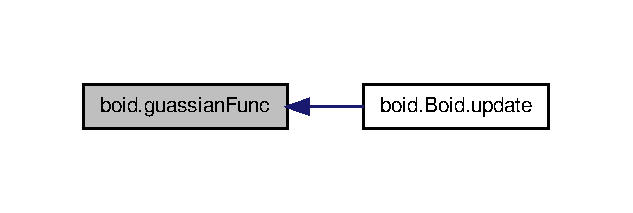
\includegraphics[width=304pt]{namespaceboid_a9986e7e6ff357ff3f6ea5f526b99f2a7_icgraph}
\end{center}
\end{figure}




\subsection{Variable Documentation}
\hypertarget{namespaceboid_a45f52f4d0bce17d64ddb37463a344776}{\index{boid@{boid}!\-\_\-\-\_\-author\-\_\-\-\_\-@{\-\_\-\-\_\-author\-\_\-\-\_\-}}
\index{\-\_\-\-\_\-author\-\_\-\-\_\-@{\-\_\-\-\_\-author\-\_\-\-\_\-}!boid@{boid}}
\subsubsection[{\-\_\-\-\_\-author\-\_\-\-\_\-}]{\setlength{\rightskip}{0pt plus 5cm}string boid.\-\_\-\-\_\-author\-\_\-\-\_\- = \char`\"{}Alex Wallar $<$aw204@st-\/andrews.\-ac.\-uk$>$\char`\"{}}}\label{namespaceboid_a45f52f4d0bce17d64ddb37463a344776}


Definition at line 3 of file boid.\-py.


\hypertarget{namespaceboidsimulation}{\section{boidsimulation Namespace Reference}
\label{namespaceboidsimulation}\index{boidsimulation@{boidsimulation}}
}
\subsection*{Classes}
\begin{DoxyCompactItemize}
\item 
class \hyperlink{classboidsimulation_1_1FlockSim}{Flock\-Sim}
\begin{DoxyCompactList}\small\item\em Main class for that is used for the simulation and display of the flock. \end{DoxyCompactList}\end{DoxyCompactItemize}
\subsection*{Variables}
\begin{DoxyCompactItemize}
\item 
string \hyperlink{namespaceboidsimulation_a70f722357d7e5a4b5ac85e726863a7ef}{\-\_\-\-\_\-author\-\_\-\-\_\-} = \char`\"{}Alex Wallar $<$aw204@st-\/andrews.\-ac.\-uk$>$\char`\"{}
\end{DoxyCompactItemize}


\subsection{Variable Documentation}
\hypertarget{namespaceboidsimulation_a70f722357d7e5a4b5ac85e726863a7ef}{\index{boidsimulation@{boidsimulation}!\-\_\-\-\_\-author\-\_\-\-\_\-@{\-\_\-\-\_\-author\-\_\-\-\_\-}}
\index{\-\_\-\-\_\-author\-\_\-\-\_\-@{\-\_\-\-\_\-author\-\_\-\-\_\-}!boidsimulation@{boidsimulation}}
\subsubsection[{\-\_\-\-\_\-author\-\_\-\-\_\-}]{\setlength{\rightskip}{0pt plus 5cm}string boidsimulation.\-\_\-\-\_\-author\-\_\-\-\_\- = \char`\"{}Alex Wallar $<$aw204@st-\/andrews.\-ac.\-uk$>$\char`\"{}}}\label{namespaceboidsimulation_a70f722357d7e5a4b5ac85e726863a7ef}


Definition at line 4 of file boidsimulation.\-py.


\hypertarget{namespaceconfiguration}{\section{configuration Namespace Reference}
\label{namespaceconfiguration}\index{configuration@{configuration}}
}
\subsection*{Classes}
\begin{DoxyCompactItemize}
\item 
class \hyperlink{classconfiguration_1_1Configuration}{Configuration}
\begin{DoxyCompactList}\small\item\em Static class that holds important global variables. \end{DoxyCompactList}\item 
class \hyperlink{classconfiguration_1_1PolyFileConfiguration}{Poly\-File\-Configuration}
\begin{DoxyCompactList}\small\item\em Extends the \hyperlink{classconfiguration_1_1Configuration}{Configuration} class. \end{DoxyCompactList}\end{DoxyCompactItemize}

\hypertarget{namespacedijkstra}{\section{dijkstra Namespace Reference}
\label{namespacedijkstra}\index{dijkstra@{dijkstra}}
}
\subsection*{Functions}
\begin{DoxyCompactItemize}
\item 
def \hyperlink{namespacedijkstra_abb1e685c821d7000ea0f6a867070443d}{Dijkstra}
\begin{DoxyCompactList}\small\item\em Find shortest paths from the start vertex to all vertices nearer than or equal to the end. \end{DoxyCompactList}\item 
def \hyperlink{namespacedijkstra_a20424eb142377bdf202ef03812875d83}{shortest\-Path}
\begin{DoxyCompactList}\small\item\em Find a single shortest path from the given start vertex to the given end vertex. \end{DoxyCompactList}\end{DoxyCompactItemize}


\subsection{Function Documentation}
\hypertarget{namespacedijkstra_abb1e685c821d7000ea0f6a867070443d}{\index{dijkstra@{dijkstra}!Dijkstra@{Dijkstra}}
\index{Dijkstra@{Dijkstra}!dijkstra@{dijkstra}}
\subsubsection[{Dijkstra}]{\setlength{\rightskip}{0pt plus 5cm}def dijkstra.\-Dijkstra (
\begin{DoxyParamCaption}
\item[{}]{G, }
\item[{}]{start, }
\item[{}]{end = {\ttfamily None}}
\end{DoxyParamCaption}
)}}\label{namespacedijkstra_abb1e685c821d7000ea0f6a867070443d}


Find shortest paths from the start vertex to all vertices nearer than or equal to the end. 

\begin{DoxyVerb} The input graph G is assumed to have the following
 representation: A vertex can be any object that can
 be used as an index into a dictionary.  G is a
 dictionary, indexed by vertices.  For any vertex v,
 G[v] is itself a dictionary, indexed by the neighbors
 of v.  For any edge v->w, G[v][w] is the length of
 the edge.  This is related to the representation in
 <http://www.python.org/doc/essays/graphs.html>
 where Guido van Rossum suggests representing graphs
 as dictionaries mapping vertices to lists of neighbors,
 however dictionaries of edges have many advantages
 over lists: they can store extra information (here,
 the lengths), they support fast existence tests,
 and they allow easy modification of the graph by edge
 insertion and removal.  Such modifications are not
 needed here but are important in other graph algorithms.
 Since dictionaries obey iterator protocol, a graph
 represented as described here could be handed without
 modification to an algorithm using Guido's representation.

 Of course, G and G[v] need not be Python dict objects;
 they can be any other object that obeys dict protocol,
 for instance a wrapper in which vertices are URLs
 and a call to G[v] loads the web page and finds its links.

 The output is a pair (D,P) where D[v] is the distance
 from start to v and P[v] is the predecessor of v along
 the shortest path from s to v.

 Dijkstra's algorithm is only guaranteed to work correctly
 when all edge lengths are positive. This code does not
 verify this property for all edges (only the edges seen
 before the end vertex is reached), but will correctly
 compute shortest paths even for some graphs with negative
 edges, and will raise an exception if it discovers that
 a negative edge has caused it to make a mistake.
\end{DoxyVerb}
 
\begin{DoxyParams}{Parameters}
{\em G} & The graph dictionary to be searched \\
\hline
{\em start} & Starting node \\
\hline
{\em end} & End node \\
\hline
\end{DoxyParams}
\begin{DoxyReturn}{Returns}
Something important 
\end{DoxyReturn}


Definition at line 53 of file dijkstra.\-py.



Here is the caller graph for this function\-:
\nopagebreak
\begin{figure}[H]
\begin{center}
\leavevmode
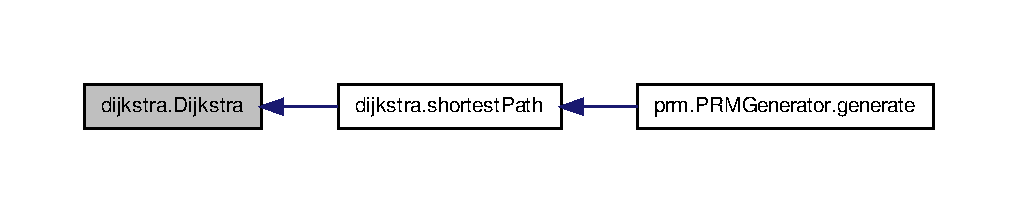
\includegraphics[width=350pt]{namespacedijkstra_abb1e685c821d7000ea0f6a867070443d_icgraph}
\end{center}
\end{figure}


\hypertarget{namespacedijkstra_a20424eb142377bdf202ef03812875d83}{\index{dijkstra@{dijkstra}!shortest\-Path@{shortest\-Path}}
\index{shortest\-Path@{shortest\-Path}!dijkstra@{dijkstra}}
\subsubsection[{shortest\-Path}]{\setlength{\rightskip}{0pt plus 5cm}def dijkstra.\-shortest\-Path (
\begin{DoxyParamCaption}
\item[{}]{G, }
\item[{}]{start, }
\item[{}]{end}
\end{DoxyParamCaption}
)}}\label{namespacedijkstra_a20424eb142377bdf202ef03812875d83}


Find a single shortest path from the given start vertex to the given end vertex. 

\begin{DoxyVerb} The input has the same conventions as Dijkstra().
 The output is a list of the vertices in order along
 the shortest path.
\end{DoxyVerb}
 
\begin{DoxyParams}{Parameters}
{\em G} & The graph dictionary to be searched \\
\hline
{\em start} & The starting node \\
\hline
{\em end} & The ending node \\
\hline
\end{DoxyParams}
\begin{DoxyReturn}{Returns}
A list of the nodes that lie on the shortest path from start to end in G 
\end{DoxyReturn}


Definition at line 89 of file dijkstra.\-py.



Here is the call graph for this function\-:\nopagebreak
\begin{figure}[H]
\begin{center}
\leavevmode
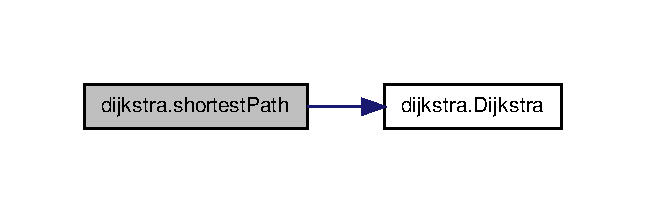
\includegraphics[width=310pt]{namespacedijkstra_a20424eb142377bdf202ef03812875d83_cgraph}
\end{center}
\end{figure}




Here is the caller graph for this function\-:
\nopagebreak
\begin{figure}[H]
\begin{center}
\leavevmode
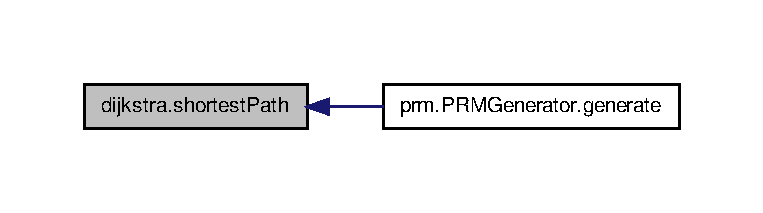
\includegraphics[width=350pt]{namespacedijkstra_a20424eb142377bdf202ef03812875d83_icgraph}
\end{center}
\end{figure}



\hypertarget{namespacegatherstats}{\section{gatherstats Namespace Reference}
\label{namespacegatherstats}\index{gatherstats@{gatherstats}}
}
\subsection*{Functions}
\begin{DoxyCompactItemize}
\item 
def \hyperlink{namespacegatherstats_ad43ef3451dcba9a62629fcdd81fd12fd}{generate\-Stats}
\begin{DoxyCompactList}\small\item\em Generates the statistics and saves them in a well known location. \end{DoxyCompactList}\end{DoxyCompactItemize}
\subsection*{Variables}
\begin{DoxyCompactItemize}
\item 
list \hyperlink{namespacegatherstats_ab219c0341d8413916db5431206ab75d9}{map\-List}
\begin{DoxyCompactList}\small\item\em A list of dictionaries used to store the map files, starting and ending points of the boids. \end{DoxyCompactList}\item 
\hyperlink{namespacegatherstats_abde74a0330bb766cc02eba7046e5f238}{test\-List} = \hyperlink{namespacegatherstats_ab219c0341d8413916db5431206ab75d9}{map\-List}
\end{DoxyCompactItemize}


\subsection{Function Documentation}
\hypertarget{namespacegatherstats_ad43ef3451dcba9a62629fcdd81fd12fd}{\index{gatherstats@{gatherstats}!generate\-Stats@{generate\-Stats}}
\index{generate\-Stats@{generate\-Stats}!gatherstats@{gatherstats}}
\subsubsection[{generate\-Stats}]{\setlength{\rightskip}{0pt plus 5cm}def gatherstats.\-generate\-Stats (
\begin{DoxyParamCaption}
\item[{}]{map\-File, }
\item[{}]{iterations, }
\item[{}]{start\-Point, }
\item[{}]{end\-Point}
\end{DoxyParamCaption}
)}}\label{namespacegatherstats_ad43ef3451dcba9a62629fcdd81fd12fd}


Generates the statistics and saves them in a well known location. 


\begin{DoxyParams}{Parameters}
{\em map\-File} & The file that stores information about the environment \\
\hline
{\em iterations} & the number of experiments to run per number of bots \\
\hline
{\em start\-Point,end\-Point} & Defines the starting and ending points of the flock \\
\hline
\end{DoxyParams}


Definition at line 14 of file gatherstats.\-py.



\subsection{Variable Documentation}
\hypertarget{namespacegatherstats_ab219c0341d8413916db5431206ab75d9}{\index{gatherstats@{gatherstats}!map\-List@{map\-List}}
\index{map\-List@{map\-List}!gatherstats@{gatherstats}}
\subsubsection[{map\-List}]{\setlength{\rightskip}{0pt plus 5cm}list gatherstats.\-map\-List}}\label{namespacegatherstats_ab219c0341d8413916db5431206ab75d9}


A list of dictionaries used to store the map files, starting and ending points of the boids. 



Definition at line 47 of file gatherstats.\-py.

\hypertarget{namespacegatherstats_abde74a0330bb766cc02eba7046e5f238}{\index{gatherstats@{gatherstats}!test\-List@{test\-List}}
\index{test\-List@{test\-List}!gatherstats@{gatherstats}}
\subsubsection[{test\-List}]{\setlength{\rightskip}{0pt plus 5cm}gatherstats.\-test\-List = {\bf map\-List}}}\label{namespacegatherstats_abde74a0330bb766cc02eba7046e5f238}


Definition at line 81 of file gatherstats.\-py.


\hypertarget{namespacegoal}{\section{goal Namespace Reference}
\label{namespacegoal}\index{goal@{goal}}
}
\subsection*{Classes}
\begin{DoxyCompactItemize}
\item 
class \hyperlink{classgoal_1_1CircleGoal}{Circle\-Goal}
\begin{DoxyCompactList}\small\item\em Object that holds data about a goal modelled as circular configuration space. \end{DoxyCompactList}\end{DoxyCompactItemize}
\subsection*{Variables}
\begin{DoxyCompactItemize}
\item 
string \hyperlink{namespacegoal_ae04fc72068c7219ebcba5f692ad7457c}{\-\_\-\-\_\-author\-\_\-\-\_\-} = \char`\"{}Alex Wallar $<$aw204@st-\/andrews.\-ac.\-uk$>$\char`\"{}
\end{DoxyCompactItemize}


\subsection{Variable Documentation}
\hypertarget{namespacegoal_ae04fc72068c7219ebcba5f692ad7457c}{\index{goal@{goal}!\-\_\-\-\_\-author\-\_\-\-\_\-@{\-\_\-\-\_\-author\-\_\-\-\_\-}}
\index{\-\_\-\-\_\-author\-\_\-\-\_\-@{\-\_\-\-\_\-author\-\_\-\-\_\-}!goal@{goal}}
\subsubsection[{\-\_\-\-\_\-author\-\_\-\-\_\-}]{\setlength{\rightskip}{0pt plus 5cm}string goal.\-\_\-\-\_\-author\-\_\-\-\_\- = \char`\"{}Alex Wallar $<$aw204@st-\/andrews.\-ac.\-uk$>$\char`\"{}}}\label{namespacegoal_ae04fc72068c7219ebcba5f692ad7457c}


Definition at line 3 of file goal.\-py.


\hypertarget{namespacemapparser}{\section{mapparser Namespace Reference}
\label{namespacemapparser}\index{mapparser@{mapparser}}
}
\subsection*{Functions}
\begin{DoxyCompactItemize}
\item 
def \hyperlink{namespacemapparser_ae6c8103aea02c5ccf436f233de9076ff}{map\-Val}
\begin{DoxyCompactList}\small\item\em Maps a value that is between in\-\_\-min and in\-\_\-max to a value between out\-\_\-min and out\-\_\-max. \end{DoxyCompactList}\item 
def \hyperlink{namespacemapparser_a6579236bba8a001573466604b1f7b398}{mparse}
\begin{DoxyCompactList}\small\item\em Parses a map file into a list of obstacles. \end{DoxyCompactList}\end{DoxyCompactItemize}


\subsection{Function Documentation}
\hypertarget{namespacemapparser_ae6c8103aea02c5ccf436f233de9076ff}{\index{mapparser@{mapparser}!map\-Val@{map\-Val}}
\index{map\-Val@{map\-Val}!mapparser@{mapparser}}
\subsubsection[{map\-Val}]{\setlength{\rightskip}{0pt plus 5cm}def mapparser.\-map\-Val (
\begin{DoxyParamCaption}
\item[{}]{x, }
\item[{}]{in\-\_\-min, }
\item[{}]{in\-\_\-max, }
\item[{}]{out\-\_\-min, }
\item[{}]{out\-\_\-max}
\end{DoxyParamCaption}
)}}\label{namespacemapparser_ae6c8103aea02c5ccf436f233de9076ff}


Maps a value that is between in\-\_\-min and in\-\_\-max to a value between out\-\_\-min and out\-\_\-max. 


\begin{DoxyParams}{Parameters}
{\em in\-\_\-min} & The minimum value that the input value could be \\
\hline
{\em in\-\_\-max} & The maximum value that the input value could be \\
\hline
{\em out\-\_\-min} & The minimum value that the output value could be \\
\hline
{\em out\-\_\-max} & The maximum value that the output value could be \\
\hline
\end{DoxyParams}
\begin{DoxyReturn}{Returns}
A scaled value based on a given input 
\end{DoxyReturn}


Definition at line 15 of file mapparser.\-py.



Here is the caller graph for this function\-:
\nopagebreak
\begin{figure}[H]
\begin{center}
\leavevmode
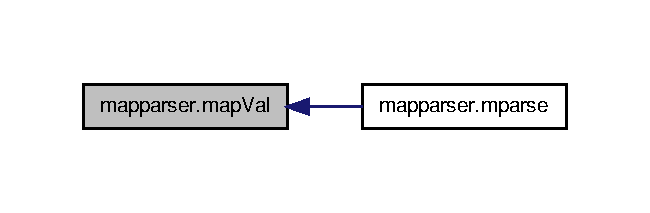
\includegraphics[width=312pt]{namespacemapparser_ae6c8103aea02c5ccf436f233de9076ff_icgraph}
\end{center}
\end{figure}


\hypertarget{namespacemapparser_a6579236bba8a001573466604b1f7b398}{\index{mapparser@{mapparser}!mparse@{mparse}}
\index{mparse@{mparse}!mapparser@{mapparser}}
\subsubsection[{mparse}]{\setlength{\rightskip}{0pt plus 5cm}def mapparser.\-mparse (
\begin{DoxyParamCaption}
\item[{}]{filename}
\end{DoxyParamCaption}
)}}\label{namespacemapparser_a6579236bba8a001573466604b1f7b398}


Parses a map file into a list of obstacles. 


\begin{DoxyParams}{Parameters}
{\em filename} & The file name of the map file \\
\hline
\end{DoxyParams}
\begin{DoxyReturn}{Returns}
A list of obstacles 
\end{DoxyReturn}


Definition at line 29 of file mapparser.\-py.



Here is the call graph for this function\-:
\nopagebreak
\begin{figure}[H]
\begin{center}
\leavevmode
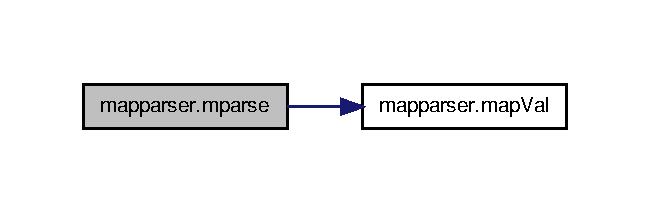
\includegraphics[width=312pt]{namespacemapparser_a6579236bba8a001573466604b1f7b398_cgraph}
\end{center}
\end{figure}



\hypertarget{namespaceobstacle}{\section{obstacle Namespace Reference}
\label{namespaceobstacle}\index{obstacle@{obstacle}}
}
\subsection*{Classes}
\begin{DoxyCompactItemize}
\item 
class \hyperlink{classobstacle_1_1PolyObstacle}{Poly\-Obstacle}
\begin{DoxyCompactList}\small\item\em Object that represents the an obstacle represented by a series of points (in the node list) which make up a set of lines. \end{DoxyCompactList}\end{DoxyCompactItemize}
\subsection*{Variables}
\begin{DoxyCompactItemize}
\item 
string \hyperlink{namespaceobstacle_a1c1558f418cc7a0e89e687fea6f31edc}{\-\_\-\-\_\-author\-\_\-\-\_\-} = \char`\"{}Alex Wallar $<$aw204@st-\/andrews.\-ac.\-uk$>$\char`\"{}
\end{DoxyCompactItemize}


\subsection{Variable Documentation}
\hypertarget{namespaceobstacle_a1c1558f418cc7a0e89e687fea6f31edc}{\index{obstacle@{obstacle}!\-\_\-\-\_\-author\-\_\-\-\_\-@{\-\_\-\-\_\-author\-\_\-\-\_\-}}
\index{\-\_\-\-\_\-author\-\_\-\-\_\-@{\-\_\-\-\_\-author\-\_\-\-\_\-}!obstacle@{obstacle}}
\subsubsection[{\-\_\-\-\_\-author\-\_\-\-\_\-}]{\setlength{\rightskip}{0pt plus 5cm}string obstacle.\-\_\-\-\_\-author\-\_\-\-\_\- = \char`\"{}Alex Wallar $<$aw204@st-\/andrews.\-ac.\-uk$>$\char`\"{}}}\label{namespaceobstacle_a1c1558f418cc7a0e89e687fea6f31edc}


Definition at line 3 of file obstacle.\-py.


\hypertarget{namespacepriodict}{\section{priodict Namespace Reference}
\label{namespacepriodict}\index{priodict@{priodict}}
}
\subsection*{Classes}
\begin{DoxyCompactItemize}
\item 
class \hyperlink{classpriodict_1_1priorityDictionary}{priority\-Dictionary}
\end{DoxyCompactItemize}

\hypertarget{namespaceprm}{\section{prm Namespace Reference}
\label{namespaceprm}\index{prm@{prm}}
}
\subsection*{Classes}
\begin{DoxyCompactItemize}
\item 
class \hyperlink{classprm_1_1PRMGenerator}{P\-R\-M\-Generator}
\begin{DoxyCompactList}\small\item\em Class used to hold methods and variables that are important for the global path planning problem. \end{DoxyCompactList}\end{DoxyCompactItemize}

\hypertarget{namespacetest__sim}{\section{test\-\_\-sim Namespace Reference}
\label{namespacetest__sim}\index{test\-\_\-sim@{test\-\_\-sim}}
}
\subsection*{Variables}
\begin{DoxyCompactItemize}
\item 
dictionary \hyperlink{namespacetest__sim_a7550c4b395516fd2fa13ebfd927c9908}{map\-Dict}
\begin{DoxyCompactList}\small\item\em Main module to run for testing purposes. \end{DoxyCompactList}\item 
tuple \hyperlink{namespacetest__sim_a2054957d15e42445f7dc826058f9799d}{fs}
\end{DoxyCompactItemize}


\subsection{Variable Documentation}
\hypertarget{namespacetest__sim_a2054957d15e42445f7dc826058f9799d}{\index{test\-\_\-sim@{test\-\_\-sim}!fs@{fs}}
\index{fs@{fs}!test_sim@{test\-\_\-sim}}
\subsubsection[{fs}]{\setlength{\rightskip}{0pt plus 5cm}tuple test\-\_\-sim.\-fs}}\label{namespacetest__sim_a2054957d15e42445f7dc826058f9799d}
{\bfseries Initial value\-:}
\begin{DoxyCode}
1 = bs.FlockSim(
2         30, 
3         mapDict[sys.argv[1]][\textcolor{stringliteral}{"startPoint"}], 
4         mapDict[sys.argv[1]][\textcolor{stringliteral}{"endPoint"}]
5     )
\end{DoxyCode}


Definition at line 24 of file test\-\_\-sim.\-py.

\hypertarget{namespacetest__sim_a7550c4b395516fd2fa13ebfd927c9908}{\index{test\-\_\-sim@{test\-\_\-sim}!map\-Dict@{map\-Dict}}
\index{map\-Dict@{map\-Dict}!test_sim@{test\-\_\-sim}}
\subsubsection[{map\-Dict}]{\setlength{\rightskip}{0pt plus 5cm}dictionary test\-\_\-sim.\-map\-Dict}}\label{namespacetest__sim_a7550c4b395516fd2fa13ebfd927c9908}
{\bfseries Initial value\-:}
\begin{DoxyCode}
1 = \{
2         \textcolor{stringliteral}{"maps/scene2.map"}: \{
3             \textcolor{stringliteral}{"startPoint"}: (494, 213), 
4             \textcolor{stringliteral}{"endPoint"}: (404, 20)
5         \}, 
6         \textcolor{stringliteral}{"maps/scene3.map"}: \{
7             \textcolor{stringliteral}{"startPoint"}: (356, 42), 
8             \textcolor{stringliteral}{"endPoint"}: (852, 450)
9         \}, 
10         \textcolor{stringliteral}{"maps/scene1.map"}: \{
11             \textcolor{stringliteral}{"startPoint"}: (50, 600), 
12             \textcolor{stringliteral}{"endPoint"}: (980, 30)
13         \}
14     \}
\end{DoxyCode}


Main module to run for testing purposes. 



Definition at line 10 of file test\-\_\-sim.\-py.


\chapter{Class Documentation}
\hypertarget{classboid_1_1Boid}{\section{boid.\-Boid Class Reference}
\label{classboid_1_1Boid}\index{boid.\-Boid@{boid.\-Boid}}
}


Class which represents one boid.  


\subsection*{Public Member Functions}
\begin{DoxyCompactItemize}
\item 
def \hyperlink{classboid_1_1Boid_adc09d58160fc982be36e29effa580536}{\-\_\-\-\_\-init\-\_\-\-\_\-}
\begin{DoxyCompactList}\small\item\em Initializes all of the variables given as input to the constructor used by the boid. \end{DoxyCompactList}\item 
def \hyperlink{classboid_1_1Boid_a9223cd4c67780cbdbe60a4efb2ee441e}{sum\-Divide}
\begin{DoxyCompactList}\small\item\em Special sort of reduce that sums components in a list of vectors and divides each final component with a certain number. \end{DoxyCompactList}\item 
def \hyperlink{classboid_1_1Boid_a576c57d100aa5743d610de30bf1a2b2c}{norm}
\begin{DoxyCompactList}\small\item\em Gets the distance between two points. \end{DoxyCompactList}\item 
def \hyperlink{classboid_1_1Boid_ab232028bea08b512bbdaab5be7dfd08f}{get\-Var}
\begin{DoxyCompactList}\small\item\em Gets multiple variables from a list with one call. \end{DoxyCompactList}\item 
def \hyperlink{classboid_1_1Boid_ab330aef12ad0a338a51a7661c736e971}{obstacle\-Func}
\begin{DoxyCompactList}\small\item\em Defines the potential between a boid and an obstacle. \end{DoxyCompactList}\item 
def \hyperlink{classboid_1_1Boid_a5324650d399f5c850ec7b7bda10eeae7}{mag}
\begin{DoxyCompactList}\small\item\em Gets the magnitude of a vector. \end{DoxyCompactList}\item 
def \hyperlink{classboid_1_1Boid_a492a0ad33a962b15ed94789d59f3b08a}{sigmoid\-Func}
\begin{DoxyCompactList}\small\item\em Defines a sigmoidal curve used for goal attraction and for boid repulsion. \end{DoxyCompactList}\item 
def \hyperlink{classboid_1_1Boid_a19392045cdd5e9b46136369028be3c52}{in\-Goal}
\begin{DoxyCompactList}\small\item\em Checks if a piont is in the current goal. \end{DoxyCompactList}\item 
def \hyperlink{classboid_1_1Boid_a321e7b1d2c37c96503e11e00ee87b96f}{in\-World}
\begin{DoxyCompactList}\small\item\em Checks if a point is in the world. \end{DoxyCompactList}\item 
def \hyperlink{classboid_1_1Boid_ae4afdcafb2e1c89390dc0648dae4c6fe}{point\-Allowed}
\begin{DoxyCompactList}\small\item\em Checks if a point is inside or collides with any of the obstacles. \end{DoxyCompactList}\item 
def \hyperlink{classboid_1_1Boid_a0df699bd295042ed4b088d94bc158f17}{init\-Function\-Parameters}
\item 
def \hyperlink{classboid_1_1Boid_ad7296706ec7c12098d3beda40c3fb283}{set\-Boid\-List}
\begin{DoxyCompactList}\small\item\em Setter method used to set the list of boids. \end{DoxyCompactList}\item 
def \hyperlink{classboid_1_1Boid_a0eb922b53c2f4e30dc0d042d1649fd2c}{update\-Position\-Buffer}
\begin{DoxyCompactList}\small\item\em Updates the position buffer. \end{DoxyCompactList}\item 
def \hyperlink{classboid_1_1Boid_a3467de3698a644a484ff63a3e86f7adc}{find\-Max}
\begin{DoxyCompactList}\small\item\em Gets the n maximum values from a list. \end{DoxyCompactList}\item 
def \hyperlink{classboid_1_1Boid_a2d4f1cded412a333857bb1b8b17d3dd0}{reduce\-Weight\-Values}
\begin{DoxyCompactList}\small\item\em Works in cohesion with sum\-Divide. \end{DoxyCompactList}\item 
def \hyperlink{classboid_1_1Boid_a8aa203db69671a064a623a88dfc6b3b7}{get\-Direction\-Vector}
\begin{DoxyCompactList}\small\item\em Gets a scaled direction vector from an unscaled vector. \end{DoxyCompactList}\item 
def \hyperlink{classboid_1_1Boid_a2c496bdcc16d7db82cc0f730ce3d5264}{get\-Obstacle\-Vector\-List}
\begin{DoxyCompactList}\small\item\em Gets the potential vectors to a boid due to the repulsive obstacle field. \end{DoxyCompactList}\item 
def \hyperlink{classboid_1_1Boid_a47c28705553bd3d729212944880161d3}{get\-Goal\-Vector}
\begin{DoxyCompactList}\small\item\em Gets the potential vectors to a boid due to the attractive goal field. \end{DoxyCompactList}\item 
def \hyperlink{classboid_1_1Boid_a353fbe920fabe58a43affaf183cfcd03}{get\-Boid\-Vector\-List}
\begin{DoxyCompactList}\small\item\em Gets the potential vectors to a boid due to the repulsive boid field. \end{DoxyCompactList}\item 
def \hyperlink{classboid_1_1Boid_aa7ef63f7cc5adfdeb565c56f359b07cd}{get\-Neighbor\-Vector\-List}
\begin{DoxyCompactList}\small\item\em Gets the heading vectors of the neighbours. \end{DoxyCompactList}\item 
def \hyperlink{classboid_1_1Boid_af2f2931c5971a4447cfe179fdafe3ab5}{set\-New\-Goal}
\begin{DoxyCompactList}\small\item\em Sets the new goal. \end{DoxyCompactList}\item 
def \hyperlink{classboid_1_1Boid_ae658dd15bb05b6addce51fba0907709b}{determine\-Random\-Walk}
\begin{DoxyCompactList}\small\item\em Increments the random walk counter, changes the current goal if necessary. \end{DoxyCompactList}\item 
def \hyperlink{classboid_1_1Boid_a47bd5446027d224319a4c71fadc846f2}{determine\-New\-Path}
\begin{DoxyCompactList}\small\item\em When the boid is stuck, it reweights the roadmap and finds a new suitable path. \end{DoxyCompactList}\item 
def \hyperlink{classboid_1_1Boid_a8a354e4b7d58ced69771f3bb5f52d257}{update}
\begin{DoxyCompactList}\small\item\em Updates the boid's heading and position due to the potential fields. \end{DoxyCompactList}\item 
def \hyperlink{classboid_1_1Boid_a289cbbc12cc9c3e7445a5f37b2d88124}{draw}
\begin{DoxyCompactList}\small\item\em Draws the boid as a pygame circle in the pygame screen. \end{DoxyCompactList}\end{DoxyCompactItemize}
\subsection*{Public Attributes}
\begin{DoxyCompactItemize}
\item 
\hyperlink{classboid_1_1Boid_abce5218cbba7b3d9f12dc78bbb9dab5e}{gamma\-Func}
\begin{DoxyCompactList}\small\item\em Function used to choose a neighbour. \end{DoxyCompactList}\item 
\hyperlink{classboid_1_1Boid_ac7d14690dde12ebc05f8f5ea80e29869}{prm\-Gen}
\begin{DoxyCompactList}\small\item\em Class which holds the details about the global path planner. \end{DoxyCompactList}\item 
\hyperlink{classboid_1_1Boid_aa230e5710394a620995a3943fc9faa8d}{screen}
\begin{DoxyCompactList}\small\item\em Py\-Game screen. \end{DoxyCompactList}\item 
\hyperlink{classboid_1_1Boid_a1bff2843c74b712aba274831d0a715d4}{radius}
\begin{DoxyCompactList}\small\item\em Radius of the boid. \end{DoxyCompactList}\item 
\hyperlink{classboid_1_1Boid_afc4b725b80313dc3604ac36015f84156}{heading}
\begin{DoxyCompactList}\small\item\em Initial random heading. \end{DoxyCompactList}\item 
\hyperlink{classboid_1_1Boid_a88a68e23e37b82bfe9862d7cd79542ad}{dim}
\begin{DoxyCompactList}\small\item\em Dimensions of the screen. \end{DoxyCompactList}\item 
\hyperlink{classboid_1_1Boid_a09f8fe6b2deb64fd65cfd64fc01470b9}{y\-Size}
\item 
\hyperlink{classboid_1_1Boid_a4af115e678f7716a2eb87c573e71073c}{neighbor\-Size}
\begin{DoxyCompactList}\small\item\em Number of neighbours that will influence the boid. \end{DoxyCompactList}\item 
\hyperlink{classboid_1_1Boid_a6a2ca3d501e4b2b0d531d4d968487907}{color}
\begin{DoxyCompactList}\small\item\em Unique color used to distinguish the boid (only used in debugging and visualization) \end{DoxyCompactList}\item 
\hyperlink{classboid_1_1Boid_a4cf2a59e0efad2d71d8fee93fdd6538b}{speed}
\begin{DoxyCompactList}\small\item\em Maximum speed of the boid. \end{DoxyCompactList}\item 
\hyperlink{classboid_1_1Boid_a9db9b88d02af40d3773b034560959694}{obstacle\-List}
\begin{DoxyCompactList}\small\item\em List of obstacles that were parsed by mapparser. \end{DoxyCompactList}\item 
\hyperlink{classboid_1_1Boid_a7a3492977220ee1f7623aa9643a2fea4}{goal\-List}
\begin{DoxyCompactList}\small\item\em Goals used by the boid. \end{DoxyCompactList}\item 
\hyperlink{classboid_1_1Boid_a8a871af6fc4d19477ce4881eb9ddc629}{goal\-Counter}
\begin{DoxyCompactList}\small\item\em Used to store what goal the boid is currently looking at. \end{DoxyCompactList}\item 
\hyperlink{classboid_1_1Boid_afe8350d9d4c1eeb15a5df7337328e1c7}{goal}
\begin{DoxyCompactList}\small\item\em Initializes the current goal. \end{DoxyCompactList}\item 
\hyperlink{classboid_1_1Boid_a099882fd7d72bfd06c15ec20b0425905}{stuck}
\begin{DoxyCompactList}\small\item\em Defines if the boid is stuck. \end{DoxyCompactList}\item 
\hyperlink{classboid_1_1Boid_a92bf79dcfff9e21d33611cfc89f8823c}{s\-Pos}
\begin{DoxyCompactList}\small\item\em Starting position of the boid. \end{DoxyCompactList}\item 
\hyperlink{classboid_1_1Boid_a15b3d73058c73aed19d2e9fb0266805d}{e\-Pos}
\begin{DoxyCompactList}\small\item\em Position of the boids. \end{DoxyCompactList}\item 
\hyperlink{classboid_1_1Boid_a483cb30093bc500a6123d5a801247ad5}{position}
\begin{DoxyCompactList}\small\item\em Sets the position of the boid. \end{DoxyCompactList}\item 
\hyperlink{classboid_1_1Boid_ab6c778a50dd384fabc6aa48be04c0988}{position\-Buffer}
\begin{DoxyCompactList}\small\item\em Used to tell if the boid is stuck or not. \end{DoxyCompactList}\item 
\hyperlink{classboid_1_1Boid_a8d7aa6d57eb3589a0770af8fcbf1aa0b}{goal\-Nodes}
\item 
\hyperlink{classboid_1_1Boid_aa30539a3bd11871eda471245cd6318e2}{roadmap}
\item 
\hyperlink{classboid_1_1Boid_ae0e9562ea35dca5f6d88e132cb5dd73a}{end\-Index}
\item 
\hyperlink{classboid_1_1Boid_abc5327f9ad46170e5f57d89c2c6e18e9}{ob\-Influence\-R}
\begin{DoxyCompactList}\small\item\em The radius of influence used when filtering the number of obstacles it needs to check. \end{DoxyCompactList}\item 
\hyperlink{classboid_1_1Boid_ae1a1d62fdc0e9014df5fcb1a49d37342}{b\-Influence\-R}
\begin{DoxyCompactList}\small\item\em The radius of influence used when filtering the number of boids it needs to check. \end{DoxyCompactList}\item 
\hyperlink{classboid_1_1Boid_a222ad56335a1e1ea39dd6da9e21797c5}{ob\-Beta}
\begin{DoxyCompactList}\small\item\em Priori constant for obstacle repulsion (increasing it gives more priority to the repulsive obstacle field) \end{DoxyCompactList}\item 
\hyperlink{classboid_1_1Boid_a5090639a7e3a489c8dc83bd12b6d1653}{g\-Alpha}
\begin{DoxyCompactList}\small\item\em Scales the value returned by the sigmoid function for goal attraction. \end{DoxyCompactList}\item 
\hyperlink{classboid_1_1Boid_a2c33a265be5079b7b916be49933eccaf}{g\-Beta}
\begin{DoxyCompactList}\small\item\em Helps scale the value returned by the sigmoid function for goal attraction. \end{DoxyCompactList}\item 
\hyperlink{classboid_1_1Boid_a17cd80cfac0fb27106c12e45929f9a9f}{g\-Delta}
\begin{DoxyCompactList}\small\item\em Constant that is used in the sigmoidal curve for goal attraction. \end{DoxyCompactList}\item 
\hyperlink{classboid_1_1Boid_a71d768a5bc70ecfcaec719cfd0c310ef}{g\-Const}
\begin{DoxyCompactList}\small\item\em Priori constant for goal attraction (increasing it gives more priority to the attractive goal field) \end{DoxyCompactList}\item 
\hyperlink{classboid_1_1Boid_abc7224afe02b42ee1c32ecd15d1b0a22}{b\-Alpha}
\begin{DoxyCompactList}\small\item\em Scales the value returned by the sigmoid function for boid repulsion. \end{DoxyCompactList}\item 
\hyperlink{classboid_1_1Boid_a1a48be012c505eea2e1b9f110d9bd5f3}{b\-Beta}
\begin{DoxyCompactList}\small\item\em Helps scale the value returned by the sigmoid function for boid repulsion. \end{DoxyCompactList}\item 
\hyperlink{classboid_1_1Boid_afebd87123c129406ee9e8c99f85f66a7}{b\-Delta}
\begin{DoxyCompactList}\small\item\em Constant that is used in the sigmoid curve for boid repulsion. \end{DoxyCompactList}\item 
\hyperlink{classboid_1_1Boid_a868b1d8e6fadd2b1beedc1a9f23edde5}{b\-Const}
\begin{DoxyCompactList}\small\item\em Priroi constant for boid repulsion (increasing it gives more priority to the repulsive boid field) \end{DoxyCompactList}\item 
\hyperlink{classboid_1_1Boid_abbcf546137204a45278b6caa95c4378b}{stuck\-Const}
\begin{DoxyCompactList}\small\item\em Amount of movement in the position buffer needs to be less that this value for a boid to be considered stuck. \end{DoxyCompactList}\item 
\hyperlink{classboid_1_1Boid_a663164af1a20323f49e002d7576914f7}{stuck\-D\-Avg}
\begin{DoxyCompactList}\small\item\em The average distance from a neighbour when a boid is stuck. \end{DoxyCompactList}\item 
\hyperlink{classboid_1_1Boid_a03960faefd59c4a651442eb373aa5c15}{stuck\-D\-Sigma}
\begin{DoxyCompactList}\small\item\em The standard deviation for a neighbour probability distribution Helps boid pick closer neighbours when it is stuck. \end{DoxyCompactList}\item 
\hyperlink{classboid_1_1Boid_acdfca1dc9b177a512502c6af681bfa9e}{n\-Stuck\-D\-Avg}
\begin{DoxyCompactList}\small\item\em The average distance from a neighbour when a boid is not stuck. \end{DoxyCompactList}\item 
\hyperlink{classboid_1_1Boid_add42a1be4f79d1ae8990065fa7e5d4de}{n\-Stuck\-D\-Sigma}
\begin{DoxyCompactList}\small\item\em The standard deviation in a neighbour distance distribution when the boid is not stuck. \end{DoxyCompactList}\item 
\hyperlink{classboid_1_1Boid_a996d92e215eb56d98a811c86c7118637}{random\-Walk\-X}
\begin{DoxyCompactList}\small\item\em Maximum x random walk. \end{DoxyCompactList}\item 
\hyperlink{classboid_1_1Boid_a1bf0149b7eadf9e6a0f08c93d95bac73}{random\-Walk\-Y}
\begin{DoxyCompactList}\small\item\em Maximum y random walk. \end{DoxyCompactList}\item 
\hyperlink{classboid_1_1Boid_af0bd96c51b17bc6c3f6fec2891b58a3d}{rand\-Walk\-Count}
\begin{DoxyCompactList}\small\item\em Stores the number of times a random walk has occurred. \end{DoxyCompactList}\item 
\hyperlink{classboid_1_1Boid_a4b192d2b077b52005a82df5d98748190}{head\-Weight\-List}
\begin{DoxyCompactList}\small\item\em Weights how much the previous heading affects the new heading. \end{DoxyCompactList}\item 
\hyperlink{classboid_1_1Boid_a6d3a16e56bd3cc7efabf9ac7cae4ae16}{boid\-List}
\item 
\hyperlink{classboid_1_1Boid_a811abb81b81e3b3e8e08e77a908ddb58}{comp\-Weight\-List}
\end{DoxyCompactItemize}


\subsection{Detailed Description}
Class which represents one boid. 

Definition at line 30 of file boid.\-py.



\subsection{Constructor \& Destructor Documentation}
\hypertarget{classboid_1_1Boid_adc09d58160fc982be36e29effa580536}{\index{boid\-::\-Boid@{boid\-::\-Boid}!\-\_\-\-\_\-init\-\_\-\-\_\-@{\-\_\-\-\_\-init\-\_\-\-\_\-}}
\index{\-\_\-\-\_\-init\-\_\-\-\_\-@{\-\_\-\-\_\-init\-\_\-\-\_\-}!boid::Boid@{boid\-::\-Boid}}
\subsubsection[{\-\_\-\-\_\-init\-\_\-\-\_\-}]{\setlength{\rightskip}{0pt plus 5cm}def boid.\-Boid.\-\_\-\-\_\-init\-\_\-\-\_\- (
\begin{DoxyParamCaption}
\item[{}]{self, }
\item[{}]{\-\_\-s\-Pos, }
\item[{}]{\-\_\-e\-Pos, }
\item[{}]{\-\_\-speed, }
\item[{}]{\-\_\-x\-Size, }
\item[{}]{\-\_\-y\-Size, }
\item[{}]{\-\_\-neighbor\-Size, }
\item[{}]{\-\_\-gamma\-Func, }
\item[{}]{\-\_\-obstacle\-List, }
\item[{}]{\-\_\-goal\-List, }
\item[{}]{\-\_\-prm\-Gen, }
\item[{}]{\-\_\-screen, }
\item[{}]{\-\_\-color}
\end{DoxyParamCaption}
)}}\label{classboid_1_1Boid_adc09d58160fc982be36e29effa580536}


Initializes all of the variables given as input to the constructor used by the boid. 


\begin{DoxyParams}{Parameters}
{\em self} & The object pointer \\
\hline
{\em \-\_\-s\-Pos} & The starting position of the boid (some noise added when initializing the flock) \\
\hline
{\em \-\_\-e\-Pos} & The ending position of the flock \\
\hline
{\em \-\_\-x\-Size} & The size of the x axis of the pygame screen \\
\hline
{\em \-\_\-neighbour\-Size} & The number of neighbours that will influence the boid's heading \\
\hline
{\em \-\_\-obstacle\-List} & List of obstacles generated by mapparser \\
\hline
{\em \-\_\-goal\-List} & List of goals used by the boid \\
\hline
{\em \-\_\-prm\-Gen} & Object that stores all of the data about the global planner \\
\hline
{\em \-\_\-screen} & Py\-Game screen \\
\hline
{\em \-\_\-color} & Unique color used for debugging purposes \\
\hline
\end{DoxyParams}
\begin{DoxyReturn}{Returns}
An instance of a boid 
\end{DoxyReturn}


Definition at line 55 of file boid.\-py.



\subsection{Member Function Documentation}
\hypertarget{classboid_1_1Boid_a47bd5446027d224319a4c71fadc846f2}{\index{boid\-::\-Boid@{boid\-::\-Boid}!determine\-New\-Path@{determine\-New\-Path}}
\index{determine\-New\-Path@{determine\-New\-Path}!boid::Boid@{boid\-::\-Boid}}
\subsubsection[{determine\-New\-Path}]{\setlength{\rightskip}{0pt plus 5cm}def boid.\-Boid.\-determine\-New\-Path (
\begin{DoxyParamCaption}
\item[{}]{self}
\end{DoxyParamCaption}
)}}\label{classboid_1_1Boid_a47bd5446027d224319a4c71fadc846f2}


When the boid is stuck, it reweights the roadmap and finds a new suitable path. 



Definition at line 653 of file boid.\-py.



Here is the call graph for this function\-:




Here is the caller graph for this function\-:


\hypertarget{classboid_1_1Boid_ae658dd15bb05b6addce51fba0907709b}{\index{boid\-::\-Boid@{boid\-::\-Boid}!determine\-Random\-Walk@{determine\-Random\-Walk}}
\index{determine\-Random\-Walk@{determine\-Random\-Walk}!boid::Boid@{boid\-::\-Boid}}
\subsubsection[{determine\-Random\-Walk}]{\setlength{\rightskip}{0pt plus 5cm}def boid.\-Boid.\-determine\-Random\-Walk (
\begin{DoxyParamCaption}
\item[{}]{self}
\end{DoxyParamCaption}
)}}\label{classboid_1_1Boid_ae658dd15bb05b6addce51fba0907709b}


Increments the random walk counter, changes the current goal if necessary. 

\begin{DoxyReturn}{Returns}
New random walk vectors where the maximum component value is determeined by the random\-Walk fields 
\end{DoxyReturn}


Definition at line 626 of file boid.\-py.

\hypertarget{classboid_1_1Boid_a289cbbc12cc9c3e7445a5f37b2d88124}{\index{boid\-::\-Boid@{boid\-::\-Boid}!draw@{draw}}
\index{draw@{draw}!boid::Boid@{boid\-::\-Boid}}
\subsubsection[{draw}]{\setlength{\rightskip}{0pt plus 5cm}def boid.\-Boid.\-draw (
\begin{DoxyParamCaption}
\item[{}]{self}
\end{DoxyParamCaption}
)}}\label{classboid_1_1Boid_a289cbbc12cc9c3e7445a5f37b2d88124}


Draws the boid as a pygame circle in the pygame screen. 



Definition at line 768 of file boid.\-py.

\hypertarget{classboid_1_1Boid_a3467de3698a644a484ff63a3e86f7adc}{\index{boid\-::\-Boid@{boid\-::\-Boid}!find\-Max@{find\-Max}}
\index{find\-Max@{find\-Max}!boid::Boid@{boid\-::\-Boid}}
\subsubsection[{find\-Max}]{\setlength{\rightskip}{0pt plus 5cm}def boid.\-Boid.\-find\-Max (
\begin{DoxyParamCaption}
\item[{}]{self, }
\item[{}]{search\-Through, }
\item[{}]{counter}
\end{DoxyParamCaption}
)}}\label{classboid_1_1Boid_a3467de3698a644a484ff63a3e86f7adc}


Gets the n maximum values from a list. 


\begin{DoxyParams}{Parameters}
{\em search\-Through} & The list that the maximums will be extracted from \\
\hline
{\em counter} & The number of values to be extracted \\
\hline
\end{DoxyParams}
\begin{DoxyReturn}{Returns}
A list of the counter maximum values from search\-Through 
\end{DoxyReturn}


Definition at line 392 of file boid.\-py.



Here is the caller graph for this function\-:\nopagebreak
\begin{figure}[H]
\begin{center}
\leavevmode
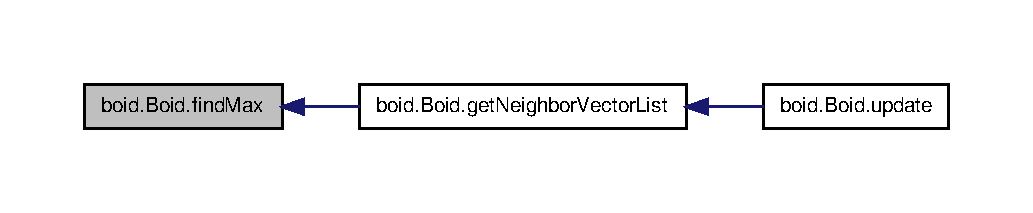
\includegraphics[width=350pt]{classboid_1_1Boid_a3467de3698a644a484ff63a3e86f7adc_icgraph}
\end{center}
\end{figure}


\hypertarget{classboid_1_1Boid_a353fbe920fabe58a43affaf183cfcd03}{\index{boid\-::\-Boid@{boid\-::\-Boid}!get\-Boid\-Vector\-List@{get\-Boid\-Vector\-List}}
\index{get\-Boid\-Vector\-List@{get\-Boid\-Vector\-List}!boid::Boid@{boid\-::\-Boid}}
\subsubsection[{get\-Boid\-Vector\-List}]{\setlength{\rightskip}{0pt plus 5cm}def boid.\-Boid.\-get\-Boid\-Vector\-List (
\begin{DoxyParamCaption}
\item[{}]{self}
\end{DoxyParamCaption}
)}}\label{classboid_1_1Boid_a353fbe920fabe58a43affaf183cfcd03}


Gets the potential vectors to a boid due to the repulsive boid field. 

\begin{DoxyReturn}{Returns}
A list of scaled vectors that will be used to determine the influence of the boids on the heading. A\-Lso returns the sum of the potential 
\end{DoxyReturn}


Definition at line 521 of file boid.\-py.



Here is the call graph for this function\-:\nopagebreak
\begin{figure}[H]
\begin{center}
\leavevmode
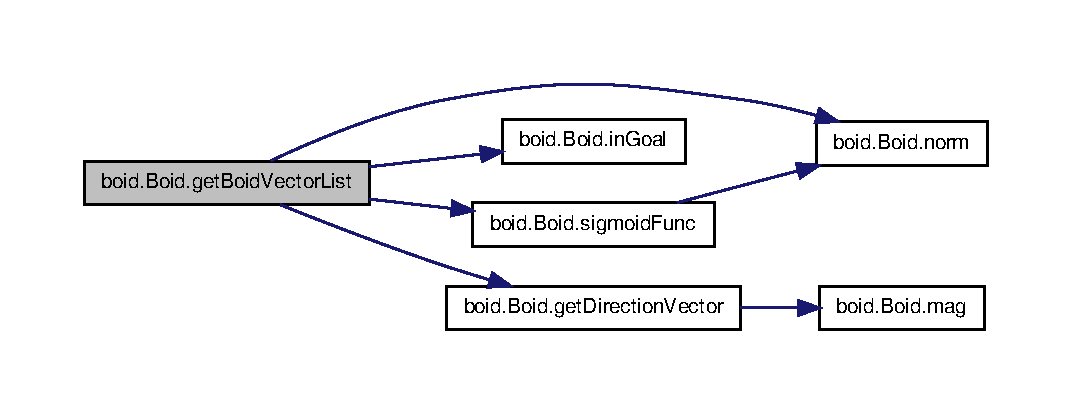
\includegraphics[width=350pt]{classboid_1_1Boid_a353fbe920fabe58a43affaf183cfcd03_cgraph}
\end{center}
\end{figure}




Here is the caller graph for this function\-:\nopagebreak
\begin{figure}[H]
\begin{center}
\leavevmode
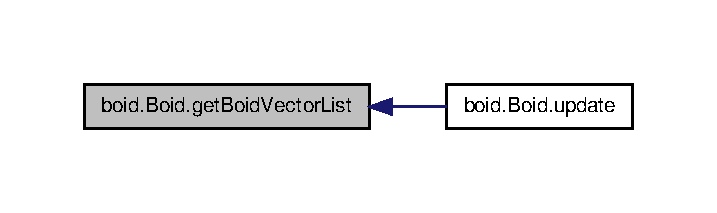
\includegraphics[width=344pt]{classboid_1_1Boid_a353fbe920fabe58a43affaf183cfcd03_icgraph}
\end{center}
\end{figure}


\hypertarget{classboid_1_1Boid_a8aa203db69671a064a623a88dfc6b3b7}{\index{boid\-::\-Boid@{boid\-::\-Boid}!get\-Direction\-Vector@{get\-Direction\-Vector}}
\index{get\-Direction\-Vector@{get\-Direction\-Vector}!boid::Boid@{boid\-::\-Boid}}
\subsubsection[{get\-Direction\-Vector}]{\setlength{\rightskip}{0pt plus 5cm}def boid.\-Boid.\-get\-Direction\-Vector (
\begin{DoxyParamCaption}
\item[{}]{self, }
\item[{}]{vector}
\end{DoxyParamCaption}
)}}\label{classboid_1_1Boid_a8aa203db69671a064a623a88dfc6b3b7}


Gets a scaled direction vector from an unscaled vector. 


\begin{DoxyParams}{Parameters}
{\em vector} & Vector to be scaled \\
\hline
\end{DoxyParams}
\begin{DoxyReturn}{Returns}
A vector whose maximum magnitude is less than the specified maximum speed 
\end{DoxyReturn}


Definition at line 425 of file boid.\-py.



Here is the call graph for this function\-:\nopagebreak
\begin{figure}[H]
\begin{center}
\leavevmode
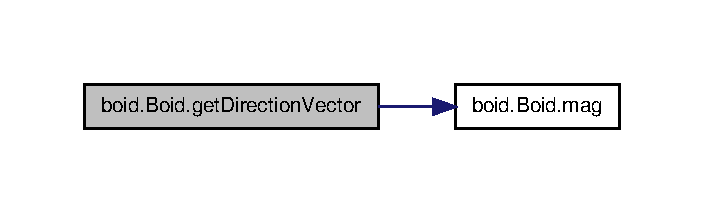
\includegraphics[width=338pt]{classboid_1_1Boid_a8aa203db69671a064a623a88dfc6b3b7_cgraph}
\end{center}
\end{figure}




Here is the caller graph for this function\-:\nopagebreak
\begin{figure}[H]
\begin{center}
\leavevmode
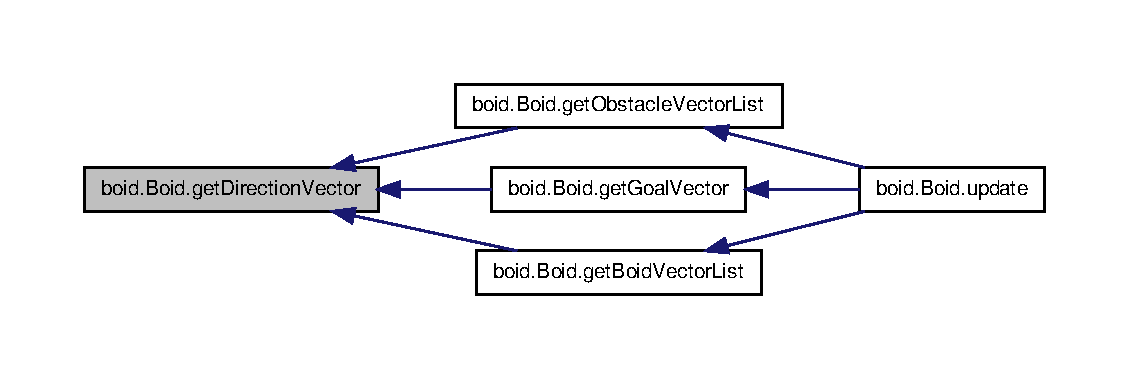
\includegraphics[width=350pt]{classboid_1_1Boid_a8aa203db69671a064a623a88dfc6b3b7_icgraph}
\end{center}
\end{figure}


\hypertarget{classboid_1_1Boid_a47c28705553bd3d729212944880161d3}{\index{boid\-::\-Boid@{boid\-::\-Boid}!get\-Goal\-Vector@{get\-Goal\-Vector}}
\index{get\-Goal\-Vector@{get\-Goal\-Vector}!boid::Boid@{boid\-::\-Boid}}
\subsubsection[{get\-Goal\-Vector}]{\setlength{\rightskip}{0pt plus 5cm}def boid.\-Boid.\-get\-Goal\-Vector (
\begin{DoxyParamCaption}
\item[{}]{self}
\end{DoxyParamCaption}
)}}\label{classboid_1_1Boid_a47c28705553bd3d729212944880161d3}


Gets the potential vectors to a boid due to the attractive goal field. 

\begin{DoxyReturn}{Returns}
A list of scaled vectors that will be used to determine the influence of the goal on the heading. Also returns the sum of the potential values 
\end{DoxyReturn}


Definition at line 490 of file boid.\-py.



Here is the call graph for this function\-:\nopagebreak
\begin{figure}[H]
\begin{center}
\leavevmode
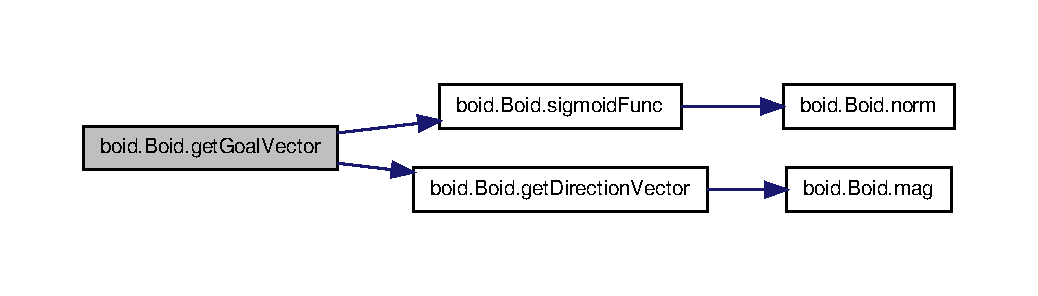
\includegraphics[width=350pt]{classboid_1_1Boid_a47c28705553bd3d729212944880161d3_cgraph}
\end{center}
\end{figure}




Here is the caller graph for this function\-:\nopagebreak
\begin{figure}[H]
\begin{center}
\leavevmode
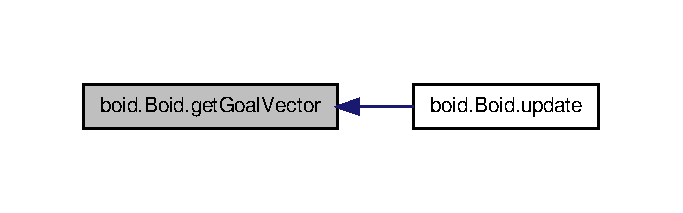
\includegraphics[width=328pt]{classboid_1_1Boid_a47c28705553bd3d729212944880161d3_icgraph}
\end{center}
\end{figure}


\hypertarget{classboid_1_1Boid_aa7ef63f7cc5adfdeb565c56f359b07cd}{\index{boid\-::\-Boid@{boid\-::\-Boid}!get\-Neighbor\-Vector\-List@{get\-Neighbor\-Vector\-List}}
\index{get\-Neighbor\-Vector\-List@{get\-Neighbor\-Vector\-List}!boid::Boid@{boid\-::\-Boid}}
\subsubsection[{get\-Neighbor\-Vector\-List}]{\setlength{\rightskip}{0pt plus 5cm}def boid.\-Boid.\-get\-Neighbor\-Vector\-List (
\begin{DoxyParamCaption}
\item[{}]{self}
\end{DoxyParamCaption}
)}}\label{classboid_1_1Boid_aa7ef63f7cc5adfdeb565c56f359b07cd}


Gets the heading vectors of the neighbours. 

\begin{DoxyReturn}{Returns}
A list of scaled vectors that represent the neighbour headings. Also returns the indicies in the boid list in which the neighbours are stored 
\end{DoxyReturn}


Definition at line 576 of file boid.\-py.



Here is the call graph for this function\-:\nopagebreak
\begin{figure}[H]
\begin{center}
\leavevmode
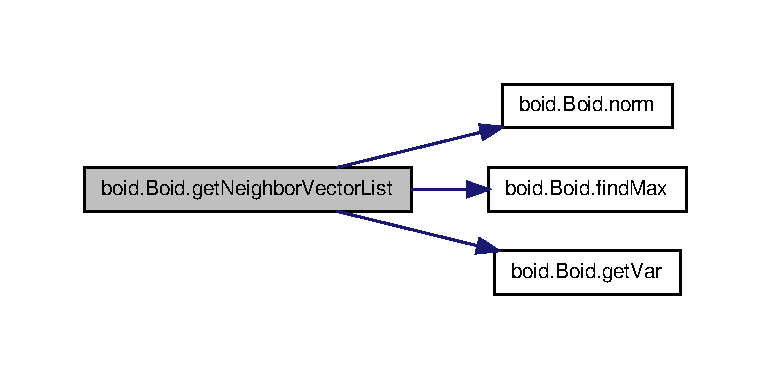
\includegraphics[width=350pt]{classboid_1_1Boid_aa7ef63f7cc5adfdeb565c56f359b07cd_cgraph}
\end{center}
\end{figure}




Here is the caller graph for this function\-:\nopagebreak
\begin{figure}[H]
\begin{center}
\leavevmode
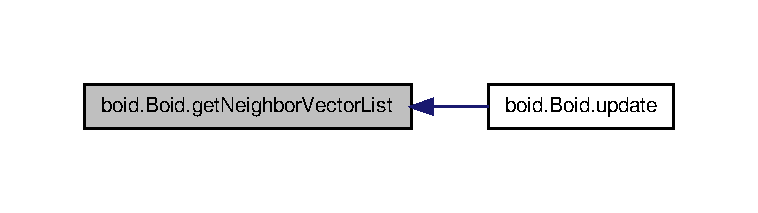
\includegraphics[width=350pt]{classboid_1_1Boid_aa7ef63f7cc5adfdeb565c56f359b07cd_icgraph}
\end{center}
\end{figure}


\hypertarget{classboid_1_1Boid_a2c496bdcc16d7db82cc0f730ce3d5264}{\index{boid\-::\-Boid@{boid\-::\-Boid}!get\-Obstacle\-Vector\-List@{get\-Obstacle\-Vector\-List}}
\index{get\-Obstacle\-Vector\-List@{get\-Obstacle\-Vector\-List}!boid::Boid@{boid\-::\-Boid}}
\subsubsection[{get\-Obstacle\-Vector\-List}]{\setlength{\rightskip}{0pt plus 5cm}def boid.\-Boid.\-get\-Obstacle\-Vector\-List (
\begin{DoxyParamCaption}
\item[{}]{self}
\end{DoxyParamCaption}
)}}\label{classboid_1_1Boid_a2c496bdcc16d7db82cc0f730ce3d5264}


Gets the potential vectors to a boid due to the repulsive obstacle field. 

\begin{DoxyReturn}{Returns}
A list of scaled vectors that will be used to determine the influence of obstacles on the heading. Also returns the sum of the potential values\begin{DoxyVerb}for ob in self.obstacleList:
    pygame.draw.circle(
self.screen,
(255,0,255),
map(int, ob.getPoint(self.position)),
2
    )
\end{DoxyVerb}
 
\end{DoxyReturn}


Definition at line 438 of file boid.\-py.



Here is the call graph for this function\-:\nopagebreak
\begin{figure}[H]
\begin{center}
\leavevmode
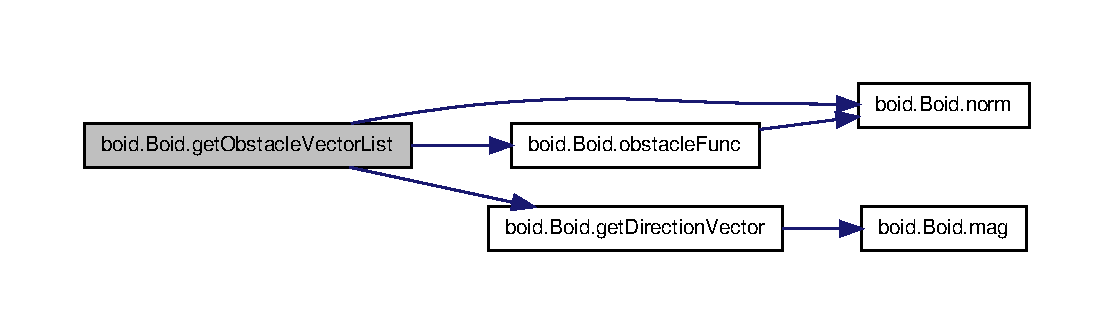
\includegraphics[width=350pt]{classboid_1_1Boid_a2c496bdcc16d7db82cc0f730ce3d5264_cgraph}
\end{center}
\end{figure}




Here is the caller graph for this function\-:\nopagebreak
\begin{figure}[H]
\begin{center}
\leavevmode
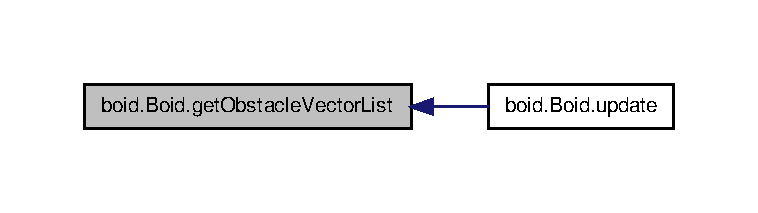
\includegraphics[width=350pt]{classboid_1_1Boid_a2c496bdcc16d7db82cc0f730ce3d5264_icgraph}
\end{center}
\end{figure}


\hypertarget{classboid_1_1Boid_ab232028bea08b512bbdaab5be7dfd08f}{\index{boid\-::\-Boid@{boid\-::\-Boid}!get\-Var@{get\-Var}}
\index{get\-Var@{get\-Var}!boid::Boid@{boid\-::\-Boid}}
\subsubsection[{get\-Var}]{\setlength{\rightskip}{0pt plus 5cm}def boid.\-Boid.\-get\-Var (
\begin{DoxyParamCaption}
\item[{}]{self, }
\item[{}]{search\-List, }
\item[{}]{ind}
\end{DoxyParamCaption}
)}}\label{classboid_1_1Boid_ab232028bea08b512bbdaab5be7dfd08f}


Gets multiple variables from a list with one call. 


\begin{DoxyParams}{Parameters}
{\em search\-List} & The list that the values will be taken from \\
\hline
{\em ind} & the indicies that will be queried \\
\hline
\end{DoxyParams}
\begin{DoxyReturn}{Returns}
A list of values from search list 
\end{DoxyReturn}


Definition at line 189 of file boid.\-py.



Here is the caller graph for this function\-:\nopagebreak
\begin{figure}[H]
\begin{center}
\leavevmode
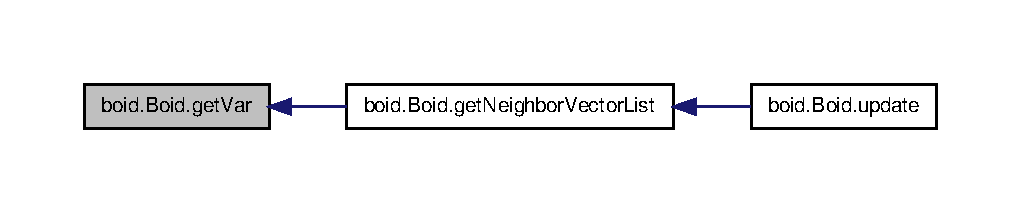
\includegraphics[width=350pt]{classboid_1_1Boid_ab232028bea08b512bbdaab5be7dfd08f_icgraph}
\end{center}
\end{figure}


\hypertarget{classboid_1_1Boid_a19392045cdd5e9b46136369028be3c52}{\index{boid\-::\-Boid@{boid\-::\-Boid}!in\-Goal@{in\-Goal}}
\index{in\-Goal@{in\-Goal}!boid::Boid@{boid\-::\-Boid}}
\subsubsection[{in\-Goal}]{\setlength{\rightskip}{0pt plus 5cm}def boid.\-Boid.\-in\-Goal (
\begin{DoxyParamCaption}
\item[{}]{self, }
\item[{}]{p}
\end{DoxyParamCaption}
)}}\label{classboid_1_1Boid_a19392045cdd5e9b46136369028be3c52}


Checks if a piont is in the current goal. 


\begin{DoxyParams}{Parameters}
{\em p} & The point that is going to be checked \\
\hline
\end{DoxyParams}
\begin{DoxyReturn}{Returns}
A boolean value representing if the point is in the current goal 
\end{DoxyReturn}


Definition at line 250 of file boid.\-py.



Here is the caller graph for this function\-:\nopagebreak
\begin{figure}[H]
\begin{center}
\leavevmode
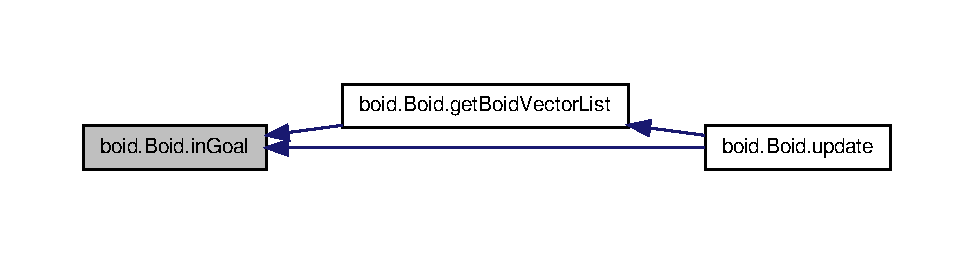
\includegraphics[width=350pt]{classboid_1_1Boid_a19392045cdd5e9b46136369028be3c52_icgraph}
\end{center}
\end{figure}


\hypertarget{classboid_1_1Boid_a0df699bd295042ed4b088d94bc158f17}{\index{boid\-::\-Boid@{boid\-::\-Boid}!init\-Function\-Parameters@{init\-Function\-Parameters}}
\index{init\-Function\-Parameters@{init\-Function\-Parameters}!boid::Boid@{boid\-::\-Boid}}
\subsubsection[{init\-Function\-Parameters}]{\setlength{\rightskip}{0pt plus 5cm}def boid.\-Boid.\-init\-Function\-Parameters (
\begin{DoxyParamCaption}
\item[{}]{self}
\end{DoxyParamCaption}
)}}\label{classboid_1_1Boid_a0df699bd295042ed4b088d94bc158f17}


Definition at line 286 of file boid.\-py.

\hypertarget{classboid_1_1Boid_a321e7b1d2c37c96503e11e00ee87b96f}{\index{boid\-::\-Boid@{boid\-::\-Boid}!in\-World@{in\-World}}
\index{in\-World@{in\-World}!boid::Boid@{boid\-::\-Boid}}
\subsubsection[{in\-World}]{\setlength{\rightskip}{0pt plus 5cm}def boid.\-Boid.\-in\-World (
\begin{DoxyParamCaption}
\item[{}]{self, }
\item[{}]{p}
\end{DoxyParamCaption}
)}}\label{classboid_1_1Boid_a321e7b1d2c37c96503e11e00ee87b96f}


Checks if a point is in the world. 


\begin{DoxyParams}{Parameters}
{\em p} & The point that is going to be checked \\
\hline
\end{DoxyParams}
\begin{DoxyReturn}{Returns}
A boolean value representing if the point is in the world 
\end{DoxyReturn}


Definition at line 265 of file boid.\-py.

\hypertarget{classboid_1_1Boid_a5324650d399f5c850ec7b7bda10eeae7}{\index{boid\-::\-Boid@{boid\-::\-Boid}!mag@{mag}}
\index{mag@{mag}!boid::Boid@{boid\-::\-Boid}}
\subsubsection[{mag}]{\setlength{\rightskip}{0pt plus 5cm}def boid.\-Boid.\-mag (
\begin{DoxyParamCaption}
\item[{}]{self, }
\item[{}]{vec}
\end{DoxyParamCaption}
)}}\label{classboid_1_1Boid_a5324650d399f5c850ec7b7bda10eeae7}


Gets the magnitude of a vector. 


\begin{DoxyParams}{Parameters}
{\em vec} & A vector represented as a list \\
\hline
\end{DoxyParams}
\begin{DoxyReturn}{Returns}
The magnitude of the vector 
\end{DoxyReturn}


Definition at line 218 of file boid.\-py.



Here is the call graph for this function\-:




Here is the caller graph for this function\-:\nopagebreak
\begin{figure}[H]
\begin{center}
\leavevmode
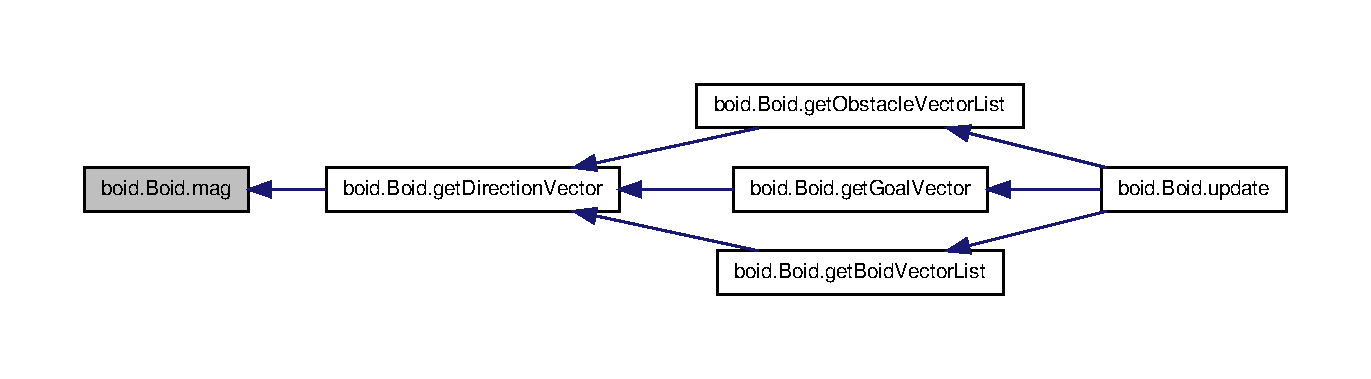
\includegraphics[width=350pt]{classboid_1_1Boid_a5324650d399f5c850ec7b7bda10eeae7_icgraph}
\end{center}
\end{figure}


\hypertarget{classboid_1_1Boid_a576c57d100aa5743d610de30bf1a2b2c}{\index{boid\-::\-Boid@{boid\-::\-Boid}!norm@{norm}}
\index{norm@{norm}!boid::Boid@{boid\-::\-Boid}}
\subsubsection[{norm}]{\setlength{\rightskip}{0pt plus 5cm}def boid.\-Boid.\-norm (
\begin{DoxyParamCaption}
\item[{}]{self, }
\item[{}]{p1, }
\item[{}]{p2}
\end{DoxyParamCaption}
)}}\label{classboid_1_1Boid_a576c57d100aa5743d610de30bf1a2b2c}


Gets the distance between two points. 


\begin{DoxyParams}{Parameters}
{\em p1,p2} & points whose distance will be returned \\
\hline
\end{DoxyParams}
\begin{DoxyReturn}{Returns}
The Euclidean distance between p1 and p2 
\end{DoxyReturn}


Definition at line 170 of file boid.\-py.



Here is the caller graph for this function\-:
\nopagebreak
\begin{figure}[H]
\begin{center}
\leavevmode
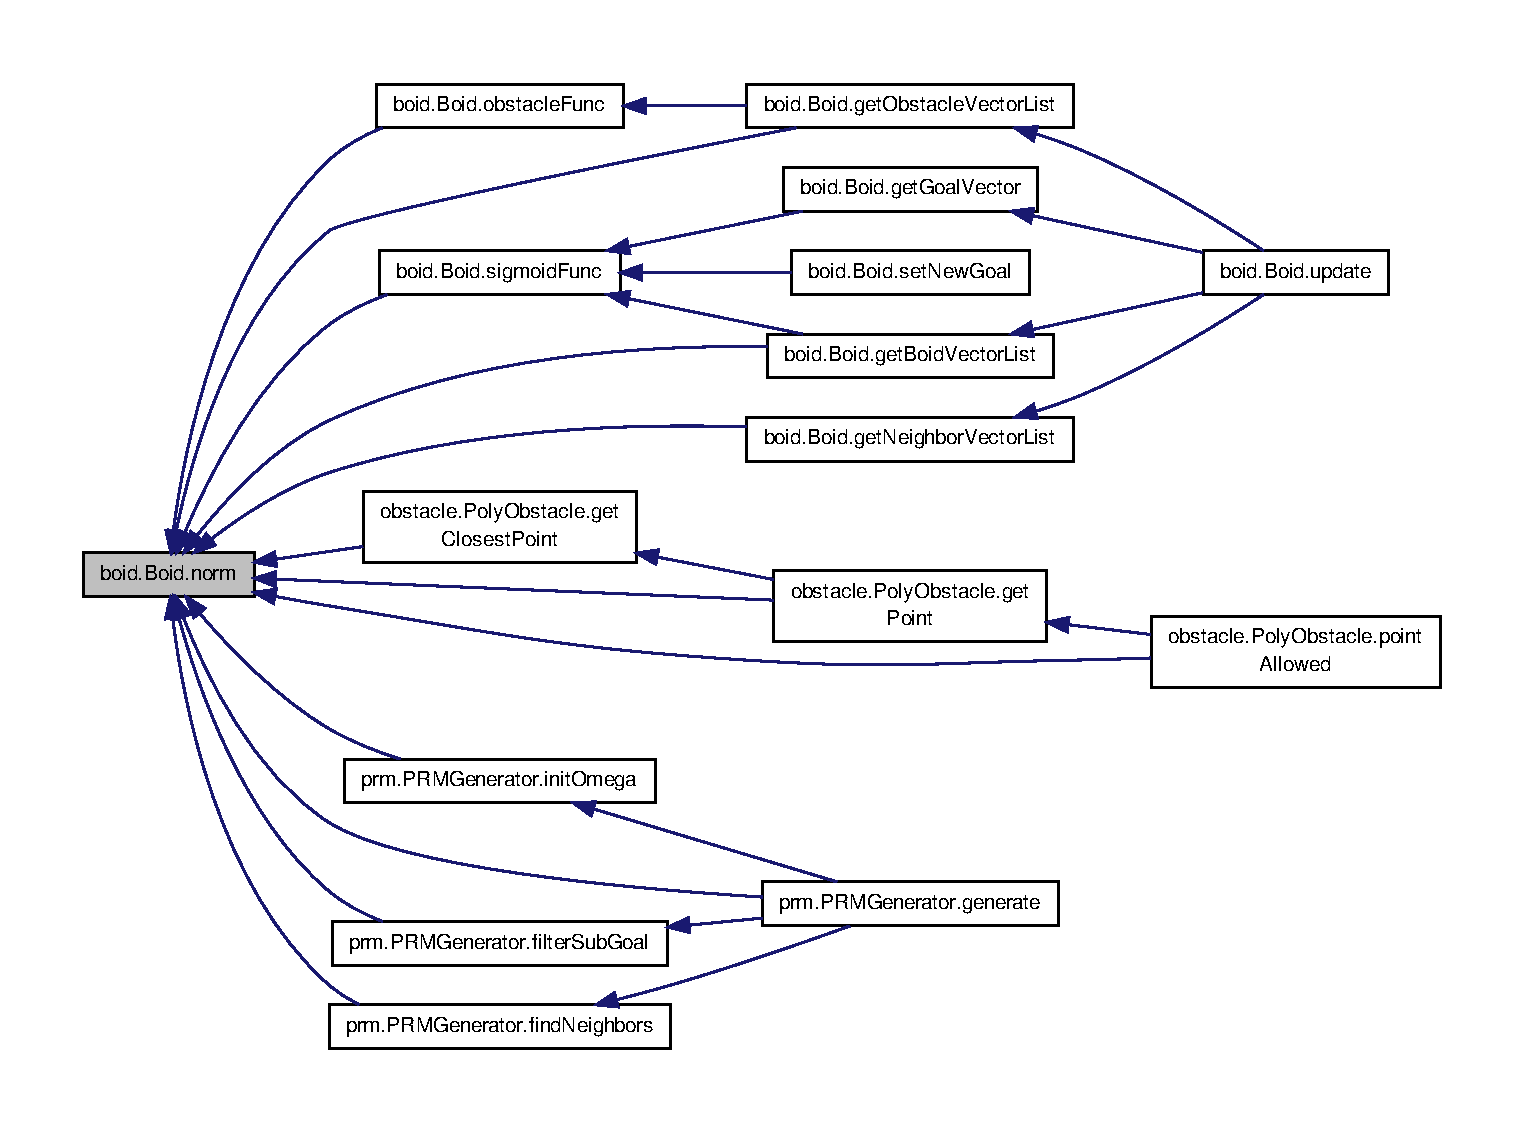
\includegraphics[width=350pt]{classboid_1_1Boid_a576c57d100aa5743d610de30bf1a2b2c_icgraph}
\end{center}
\end{figure}


\hypertarget{classboid_1_1Boid_ab330aef12ad0a338a51a7661c736e971}{\index{boid\-::\-Boid@{boid\-::\-Boid}!obstacle\-Func@{obstacle\-Func}}
\index{obstacle\-Func@{obstacle\-Func}!boid::Boid@{boid\-::\-Boid}}
\subsubsection[{obstacle\-Func}]{\setlength{\rightskip}{0pt plus 5cm}def boid.\-Boid.\-obstacle\-Func (
\begin{DoxyParamCaption}
\item[{}]{self, }
\item[{}]{beta, }
\item[{}]{b, }
\item[{}]{o}
\end{DoxyParamCaption}
)}}\label{classboid_1_1Boid_ab330aef12ad0a338a51a7661c736e971}


Defines the potential between a boid and an obstacle. 


\begin{DoxyParams}{Parameters}
{\em beta} & Constant used to increase the weight of the function \\
\hline
{\em b} & The boid that is being comapred \\
\hline
{\em o} & The obstacle that is being compared \\
\hline
\end{DoxyParams}
\begin{DoxyReturn}{Returns}
A value representing the potential between b and o 
\end{DoxyReturn}


Definition at line 200 of file boid.\-py.



Here is the call graph for this function\-:\nopagebreak
\begin{figure}[H]
\begin{center}
\leavevmode
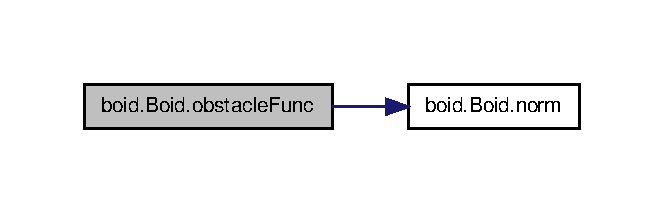
\includegraphics[width=318pt]{classboid_1_1Boid_ab330aef12ad0a338a51a7661c736e971_cgraph}
\end{center}
\end{figure}




Here is the caller graph for this function\-:\nopagebreak
\begin{figure}[H]
\begin{center}
\leavevmode
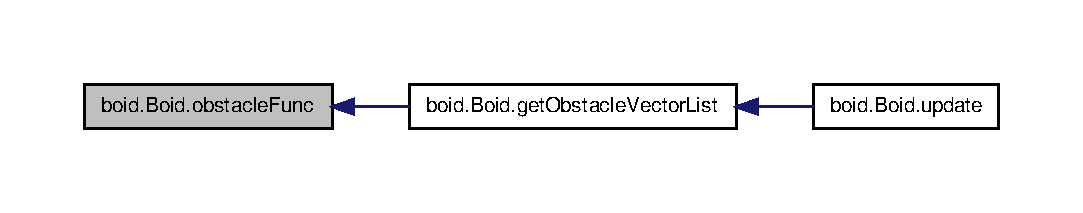
\includegraphics[width=350pt]{classboid_1_1Boid_ab330aef12ad0a338a51a7661c736e971_icgraph}
\end{center}
\end{figure}


\hypertarget{classboid_1_1Boid_ae4afdcafb2e1c89390dc0648dae4c6fe}{\index{boid\-::\-Boid@{boid\-::\-Boid}!point\-Allowed@{point\-Allowed}}
\index{point\-Allowed@{point\-Allowed}!boid::Boid@{boid\-::\-Boid}}
\subsubsection[{point\-Allowed}]{\setlength{\rightskip}{0pt plus 5cm}def boid.\-Boid.\-point\-Allowed (
\begin{DoxyParamCaption}
\item[{}]{self, }
\item[{}]{p}
\end{DoxyParamCaption}
)}}\label{classboid_1_1Boid_ae4afdcafb2e1c89390dc0648dae4c6fe}


Checks if a point is inside or collides with any of the obstacles. 


\begin{DoxyParams}{Parameters}
{\em p} & The point that will be checked \\
\hline
\end{DoxyParams}


Definition at line 278 of file boid.\-py.

\hypertarget{classboid_1_1Boid_a2d4f1cded412a333857bb1b8b17d3dd0}{\index{boid\-::\-Boid@{boid\-::\-Boid}!reduce\-Weight\-Values@{reduce\-Weight\-Values}}
\index{reduce\-Weight\-Values@{reduce\-Weight\-Values}!boid::Boid@{boid\-::\-Boid}}
\subsubsection[{reduce\-Weight\-Values}]{\setlength{\rightskip}{0pt plus 5cm}def boid.\-Boid.\-reduce\-Weight\-Values (
\begin{DoxyParamCaption}
\item[{}]{self, }
\item[{}]{w\-List, }
\item[{}]{v\-List}
\end{DoxyParamCaption}
)}}\label{classboid_1_1Boid_a2d4f1cded412a333857bb1b8b17d3dd0}


Works in cohesion with sum\-Divide. 

Weights values in a list and divides by the sum of those weights 
\begin{DoxyParams}{Parameters}
{\em w\-List} & List of Weights \\
\hline
{\em $\ast$v\-List} & Values that will be weighted \\
\hline
\end{DoxyParams}
\begin{DoxyReturn}{Returns}
An average vector that represents the average heading due to the potential fields 
\end{DoxyReturn}


Definition at line 412 of file boid.\-py.



Here is the call graph for this function\-:\nopagebreak
\begin{figure}[H]
\begin{center}
\leavevmode
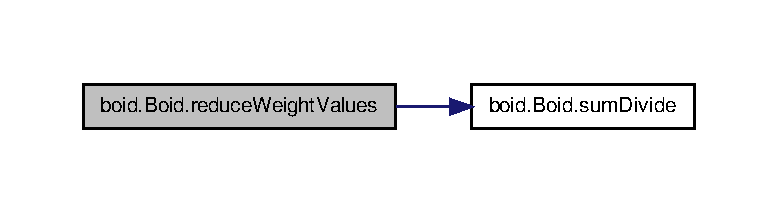
\includegraphics[width=350pt]{classboid_1_1Boid_a2d4f1cded412a333857bb1b8b17d3dd0_cgraph}
\end{center}
\end{figure}


\hypertarget{classboid_1_1Boid_ad7296706ec7c12098d3beda40c3fb283}{\index{boid\-::\-Boid@{boid\-::\-Boid}!set\-Boid\-List@{set\-Boid\-List}}
\index{set\-Boid\-List@{set\-Boid\-List}!boid::Boid@{boid\-::\-Boid}}
\subsubsection[{set\-Boid\-List}]{\setlength{\rightskip}{0pt plus 5cm}def boid.\-Boid.\-set\-Boid\-List (
\begin{DoxyParamCaption}
\item[{}]{self, }
\item[{}]{\-\_\-boid\-List}
\end{DoxyParamCaption}
)}}\label{classboid_1_1Boid_ad7296706ec7c12098d3beda40c3fb283}


Setter method used to set the list of boids. 


\begin{DoxyParams}{Parameters}
{\em \-\_\-boid\-List} & The list of boids in the flock \\
\hline
\end{DoxyParams}


Definition at line 370 of file boid.\-py.

\hypertarget{classboid_1_1Boid_af2f2931c5971a4447cfe179fdafe3ab5}{\index{boid\-::\-Boid@{boid\-::\-Boid}!set\-New\-Goal@{set\-New\-Goal}}
\index{set\-New\-Goal@{set\-New\-Goal}!boid::Boid@{boid\-::\-Boid}}
\subsubsection[{set\-New\-Goal}]{\setlength{\rightskip}{0pt plus 5cm}def boid.\-Boid.\-set\-New\-Goal (
\begin{DoxyParamCaption}
\item[{}]{self}
\end{DoxyParamCaption}
)}}\label{classboid_1_1Boid_af2f2931c5971a4447cfe179fdafe3ab5}


Sets the new goal. 



Definition at line 606 of file boid.\-py.



Here is the call graph for this function\-:\nopagebreak
\begin{figure}[H]
\begin{center}
\leavevmode
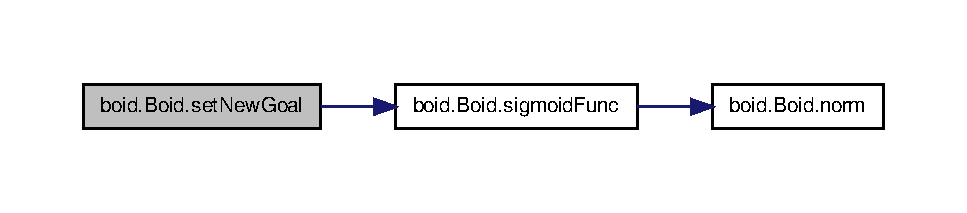
\includegraphics[width=350pt]{classboid_1_1Boid_af2f2931c5971a4447cfe179fdafe3ab5_cgraph}
\end{center}
\end{figure}


\hypertarget{classboid_1_1Boid_a492a0ad33a962b15ed94789d59f3b08a}{\index{boid\-::\-Boid@{boid\-::\-Boid}!sigmoid\-Func@{sigmoid\-Func}}
\index{sigmoid\-Func@{sigmoid\-Func}!boid::Boid@{boid\-::\-Boid}}
\subsubsection[{sigmoid\-Func}]{\setlength{\rightskip}{0pt plus 5cm}def boid.\-Boid.\-sigmoid\-Func (
\begin{DoxyParamCaption}
\item[{}]{self, }
\item[{}]{alpha, }
\item[{}]{beta, }
\item[{}]{delta, }
\item[{}]{const, }
\item[{}]{b\-\_\-r, }
\item[{}]{g\-\_\-r, }
\item[{}]{b\-\_\-pos, }
\item[{}]{g\-\_\-pos}
\end{DoxyParamCaption}
)}}\label{classboid_1_1Boid_a492a0ad33a962b15ed94789d59f3b08a}


Defines a sigmoidal curve used for goal attraction and for boid repulsion. 


\begin{DoxyParams}{Parameters}
{\em alpha,beta,delta,const} & Constants that are used to modify the shape of the curve \\
\hline
{\em b\-\_\-r,b\-\_\-pos} & The radius and position of the boid \\
\hline
{\em g\-\_\-r,g\-\_\-pos} & The radius and position of a goal / boid \\
\hline
\end{DoxyParams}


Definition at line 231 of file boid.\-py.



Here is the call graph for this function\-:\nopagebreak
\begin{figure}[H]
\begin{center}
\leavevmode
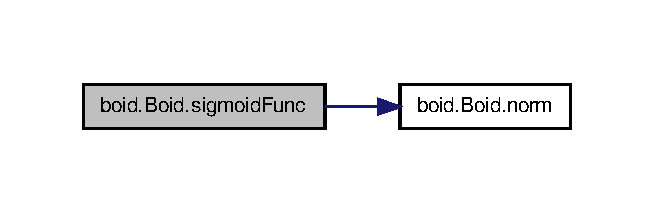
\includegraphics[width=314pt]{classboid_1_1Boid_a492a0ad33a962b15ed94789d59f3b08a_cgraph}
\end{center}
\end{figure}




Here is the caller graph for this function\-:\nopagebreak
\begin{figure}[H]
\begin{center}
\leavevmode
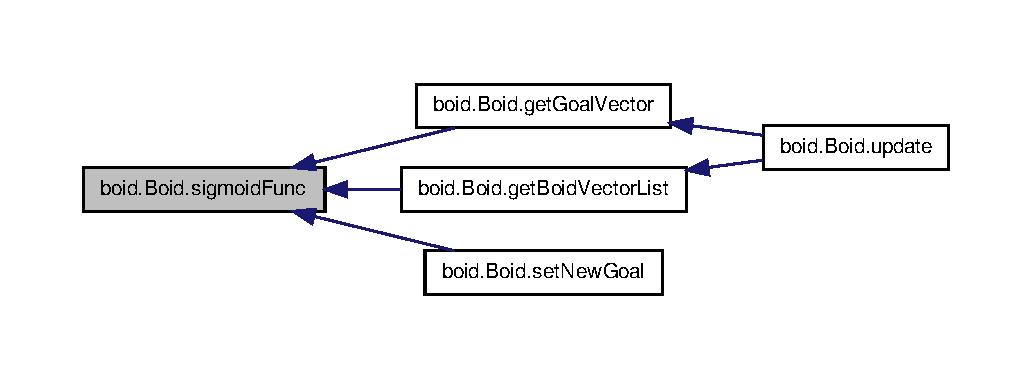
\includegraphics[width=350pt]{classboid_1_1Boid_a492a0ad33a962b15ed94789d59f3b08a_icgraph}
\end{center}
\end{figure}


\hypertarget{classboid_1_1Boid_a9223cd4c67780cbdbe60a4efb2ee441e}{\index{boid\-::\-Boid@{boid\-::\-Boid}!sum\-Divide@{sum\-Divide}}
\index{sum\-Divide@{sum\-Divide}!boid::Boid@{boid\-::\-Boid}}
\subsubsection[{sum\-Divide}]{\setlength{\rightskip}{0pt plus 5cm}def boid.\-Boid.\-sum\-Divide (
\begin{DoxyParamCaption}
\item[{}]{self, }
\item[{}]{lt, }
\item[{}]{s}
\end{DoxyParamCaption}
)}}\label{classboid_1_1Boid_a9223cd4c67780cbdbe60a4efb2ee441e}


Special sort of reduce that sums components in a list of vectors and divides each final component with a certain number. 


\begin{DoxyParams}{Parameters}
{\em self} & The object pointer \\
\hline
{\em lt} & List of vectors that will be summed over and divided \\
\hline
{\em s} & Number that will divide each component by at the end \\
\hline
\end{DoxyParams}


Definition at line 149 of file boid.\-py.



Here is the caller graph for this function\-:\nopagebreak
\begin{figure}[H]
\begin{center}
\leavevmode
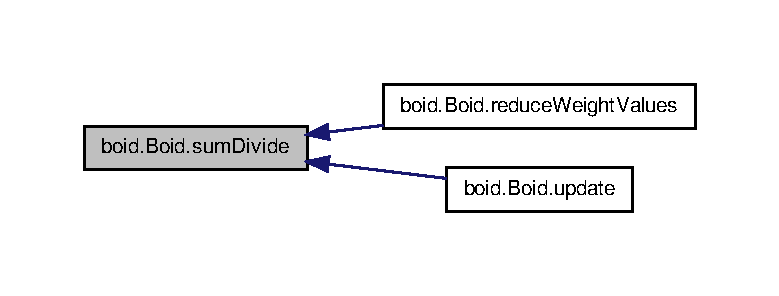
\includegraphics[width=350pt]{classboid_1_1Boid_a9223cd4c67780cbdbe60a4efb2ee441e_icgraph}
\end{center}
\end{figure}


\hypertarget{classboid_1_1Boid_a8a354e4b7d58ced69771f3bb5f52d257}{\index{boid\-::\-Boid@{boid\-::\-Boid}!update@{update}}
\index{update@{update}!boid::Boid@{boid\-::\-Boid}}
\subsubsection[{update}]{\setlength{\rightskip}{0pt plus 5cm}def boid.\-Boid.\-update (
\begin{DoxyParamCaption}
\item[{}]{self}
\end{DoxyParamCaption}
)}}\label{classboid_1_1Boid_a8a354e4b7d58ced69771f3bb5f52d257}


Updates the boid's heading and position due to the potential fields. 



Definition at line 690 of file boid.\-py.



Here is the call graph for this function\-:
\nopagebreak
\begin{figure}[H]
\begin{center}
\leavevmode
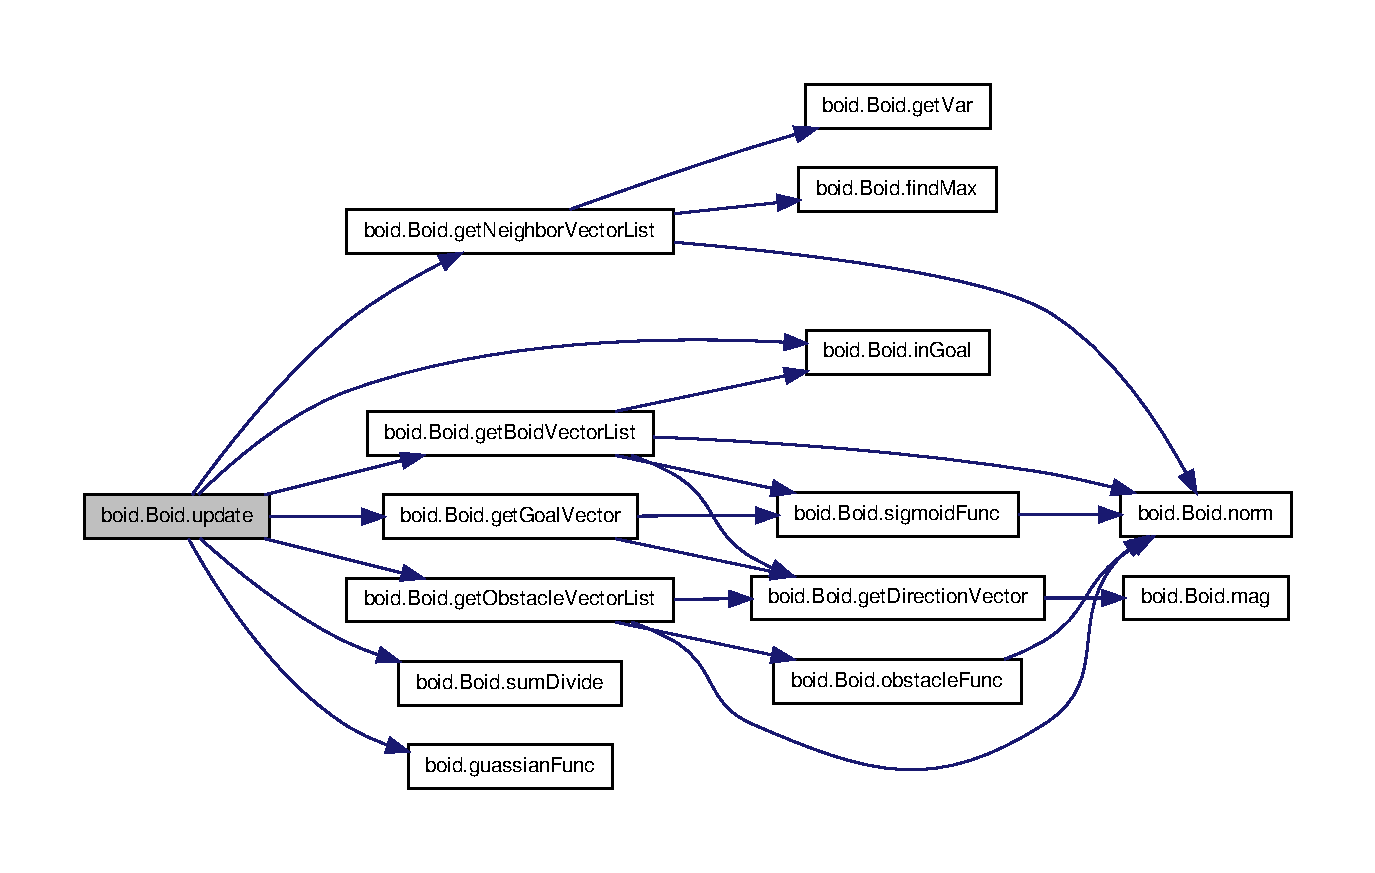
\includegraphics[width=350pt]{classboid_1_1Boid_a8a354e4b7d58ced69771f3bb5f52d257_cgraph}
\end{center}
\end{figure}


\hypertarget{classboid_1_1Boid_a0eb922b53c2f4e30dc0d042d1649fd2c}{\index{boid\-::\-Boid@{boid\-::\-Boid}!update\-Position\-Buffer@{update\-Position\-Buffer}}
\index{update\-Position\-Buffer@{update\-Position\-Buffer}!boid::Boid@{boid\-::\-Boid}}
\subsubsection[{update\-Position\-Buffer}]{\setlength{\rightskip}{0pt plus 5cm}def boid.\-Boid.\-update\-Position\-Buffer (
\begin{DoxyParamCaption}
\item[{}]{self}
\end{DoxyParamCaption}
)}}\label{classboid_1_1Boid_a0eb922b53c2f4e30dc0d042d1649fd2c}


Updates the position buffer. 

\begin{DoxyReturn}{Returns}
The displacement of a boid over a certain number of frames 
\end{DoxyReturn}


Definition at line 378 of file boid.\-py.



\subsection{Member Data Documentation}
\hypertarget{classboid_1_1Boid_abc7224afe02b42ee1c32ecd15d1b0a22}{\index{boid\-::\-Boid@{boid\-::\-Boid}!b\-Alpha@{b\-Alpha}}
\index{b\-Alpha@{b\-Alpha}!boid::Boid@{boid\-::\-Boid}}
\subsubsection[{b\-Alpha}]{\setlength{\rightskip}{0pt plus 5cm}boid.\-Boid.\-b\-Alpha}}\label{classboid_1_1Boid_abc7224afe02b42ee1c32ecd15d1b0a22}


Scales the value returned by the sigmoid function for boid repulsion. 



Definition at line 319 of file boid.\-py.

\hypertarget{classboid_1_1Boid_a1a48be012c505eea2e1b9f110d9bd5f3}{\index{boid\-::\-Boid@{boid\-::\-Boid}!b\-Beta@{b\-Beta}}
\index{b\-Beta@{b\-Beta}!boid::Boid@{boid\-::\-Boid}}
\subsubsection[{b\-Beta}]{\setlength{\rightskip}{0pt plus 5cm}boid.\-Boid.\-b\-Beta}}\label{classboid_1_1Boid_a1a48be012c505eea2e1b9f110d9bd5f3}


Helps scale the value returned by the sigmoid function for boid repulsion. 



Definition at line 323 of file boid.\-py.

\hypertarget{classboid_1_1Boid_a868b1d8e6fadd2b1beedc1a9f23edde5}{\index{boid\-::\-Boid@{boid\-::\-Boid}!b\-Const@{b\-Const}}
\index{b\-Const@{b\-Const}!boid::Boid@{boid\-::\-Boid}}
\subsubsection[{b\-Const}]{\setlength{\rightskip}{0pt plus 5cm}boid.\-Boid.\-b\-Const}}\label{classboid_1_1Boid_a868b1d8e6fadd2b1beedc1a9f23edde5}


Priroi constant for boid repulsion (increasing it gives more priority to the repulsive boid field) 



Definition at line 331 of file boid.\-py.

\hypertarget{classboid_1_1Boid_afebd87123c129406ee9e8c99f85f66a7}{\index{boid\-::\-Boid@{boid\-::\-Boid}!b\-Delta@{b\-Delta}}
\index{b\-Delta@{b\-Delta}!boid::Boid@{boid\-::\-Boid}}
\subsubsection[{b\-Delta}]{\setlength{\rightskip}{0pt plus 5cm}boid.\-Boid.\-b\-Delta}}\label{classboid_1_1Boid_afebd87123c129406ee9e8c99f85f66a7}


Constant that is used in the sigmoid curve for boid repulsion. 



Definition at line 327 of file boid.\-py.

\hypertarget{classboid_1_1Boid_ae1a1d62fdc0e9014df5fcb1a49d37342}{\index{boid\-::\-Boid@{boid\-::\-Boid}!b\-Influence\-R@{b\-Influence\-R}}
\index{b\-Influence\-R@{b\-Influence\-R}!boid::Boid@{boid\-::\-Boid}}
\subsubsection[{b\-Influence\-R}]{\setlength{\rightskip}{0pt plus 5cm}boid.\-Boid.\-b\-Influence\-R}}\label{classboid_1_1Boid_ae1a1d62fdc0e9014df5fcb1a49d37342}


The radius of influence used when filtering the number of boids it needs to check. 



Definition at line 295 of file boid.\-py.

\hypertarget{classboid_1_1Boid_a6d3a16e56bd3cc7efabf9ac7cae4ae16}{\index{boid\-::\-Boid@{boid\-::\-Boid}!boid\-List@{boid\-List}}
\index{boid\-List@{boid\-List}!boid::Boid@{boid\-::\-Boid}}
\subsubsection[{boid\-List}]{\setlength{\rightskip}{0pt plus 5cm}boid.\-Boid.\-boid\-List}}\label{classboid_1_1Boid_a6d3a16e56bd3cc7efabf9ac7cae4ae16}


Definition at line 371 of file boid.\-py.

\hypertarget{classboid_1_1Boid_a6a2ca3d501e4b2b0d531d4d968487907}{\index{boid\-::\-Boid@{boid\-::\-Boid}!color@{color}}
\index{color@{color}!boid::Boid@{boid\-::\-Boid}}
\subsubsection[{color}]{\setlength{\rightskip}{0pt plus 5cm}boid.\-Boid.\-color}}\label{classboid_1_1Boid_a6a2ca3d501e4b2b0d531d4d968487907}


Unique color used to distinguish the boid (only used in debugging and visualization) 



Definition at line 87 of file boid.\-py.

\hypertarget{classboid_1_1Boid_a811abb81b81e3b3e8e08e77a908ddb58}{\index{boid\-::\-Boid@{boid\-::\-Boid}!comp\-Weight\-List@{comp\-Weight\-List}}
\index{comp\-Weight\-List@{comp\-Weight\-List}!boid::Boid@{boid\-::\-Boid}}
\subsubsection[{comp\-Weight\-List}]{\setlength{\rightskip}{0pt plus 5cm}boid.\-Boid.\-comp\-Weight\-List}}\label{classboid_1_1Boid_a811abb81b81e3b3e8e08e77a908ddb58}


Definition at line 731 of file boid.\-py.

\hypertarget{classboid_1_1Boid_a88a68e23e37b82bfe9862d7cd79542ad}{\index{boid\-::\-Boid@{boid\-::\-Boid}!dim@{dim}}
\index{dim@{dim}!boid::Boid@{boid\-::\-Boid}}
\subsubsection[{dim}]{\setlength{\rightskip}{0pt plus 5cm}boid.\-Boid.\-dim}}\label{classboid_1_1Boid_a88a68e23e37b82bfe9862d7cd79542ad}


Dimensions of the screen. 



Definition at line 80 of file boid.\-py.

\hypertarget{classboid_1_1Boid_ae0e9562ea35dca5f6d88e132cb5dd73a}{\index{boid\-::\-Boid@{boid\-::\-Boid}!end\-Index@{end\-Index}}
\index{end\-Index@{end\-Index}!boid::Boid@{boid\-::\-Boid}}
\subsubsection[{end\-Index}]{\setlength{\rightskip}{0pt plus 5cm}boid.\-Boid.\-end\-Index}}\label{classboid_1_1Boid_ae0e9562ea35dca5f6d88e132cb5dd73a}


Definition at line 136 of file boid.\-py.

\hypertarget{classboid_1_1Boid_a15b3d73058c73aed19d2e9fb0266805d}{\index{boid\-::\-Boid@{boid\-::\-Boid}!e\-Pos@{e\-Pos}}
\index{e\-Pos@{e\-Pos}!boid::Boid@{boid\-::\-Boid}}
\subsubsection[{e\-Pos}]{\setlength{\rightskip}{0pt plus 5cm}boid.\-Boid.\-e\-Pos}}\label{classboid_1_1Boid_a15b3d73058c73aed19d2e9fb0266805d}


Position of the boids. 



Definition at line 111 of file boid.\-py.

\hypertarget{classboid_1_1Boid_a5090639a7e3a489c8dc83bd12b6d1653}{\index{boid\-::\-Boid@{boid\-::\-Boid}!g\-Alpha@{g\-Alpha}}
\index{g\-Alpha@{g\-Alpha}!boid::Boid@{boid\-::\-Boid}}
\subsubsection[{g\-Alpha}]{\setlength{\rightskip}{0pt plus 5cm}boid.\-Boid.\-g\-Alpha}}\label{classboid_1_1Boid_a5090639a7e3a489c8dc83bd12b6d1653}


Scales the value returned by the sigmoid function for goal attraction. 



Definition at line 303 of file boid.\-py.

\hypertarget{classboid_1_1Boid_abce5218cbba7b3d9f12dc78bbb9dab5e}{\index{boid\-::\-Boid@{boid\-::\-Boid}!gamma\-Func@{gamma\-Func}}
\index{gamma\-Func@{gamma\-Func}!boid::Boid@{boid\-::\-Boid}}
\subsubsection[{gamma\-Func}]{\setlength{\rightskip}{0pt plus 5cm}boid.\-Boid.\-gamma\-Func}}\label{classboid_1_1Boid_abce5218cbba7b3d9f12dc78bbb9dab5e}


Function used to choose a neighbour. 



Definition at line 58 of file boid.\-py.

\hypertarget{classboid_1_1Boid_a2c33a265be5079b7b916be49933eccaf}{\index{boid\-::\-Boid@{boid\-::\-Boid}!g\-Beta@{g\-Beta}}
\index{g\-Beta@{g\-Beta}!boid::Boid@{boid\-::\-Boid}}
\subsubsection[{g\-Beta}]{\setlength{\rightskip}{0pt plus 5cm}boid.\-Boid.\-g\-Beta}}\label{classboid_1_1Boid_a2c33a265be5079b7b916be49933eccaf}


Helps scale the value returned by the sigmoid function for goal attraction. 



Definition at line 307 of file boid.\-py.

\hypertarget{classboid_1_1Boid_a71d768a5bc70ecfcaec719cfd0c310ef}{\index{boid\-::\-Boid@{boid\-::\-Boid}!g\-Const@{g\-Const}}
\index{g\-Const@{g\-Const}!boid::Boid@{boid\-::\-Boid}}
\subsubsection[{g\-Const}]{\setlength{\rightskip}{0pt plus 5cm}boid.\-Boid.\-g\-Const}}\label{classboid_1_1Boid_a71d768a5bc70ecfcaec719cfd0c310ef}


Priori constant for goal attraction (increasing it gives more priority to the attractive goal field) 



Definition at line 315 of file boid.\-py.

\hypertarget{classboid_1_1Boid_a17cd80cfac0fb27106c12e45929f9a9f}{\index{boid\-::\-Boid@{boid\-::\-Boid}!g\-Delta@{g\-Delta}}
\index{g\-Delta@{g\-Delta}!boid::Boid@{boid\-::\-Boid}}
\subsubsection[{g\-Delta}]{\setlength{\rightskip}{0pt plus 5cm}boid.\-Boid.\-g\-Delta}}\label{classboid_1_1Boid_a17cd80cfac0fb27106c12e45929f9a9f}


Constant that is used in the sigmoidal curve for goal attraction. 



Definition at line 311 of file boid.\-py.

\hypertarget{classboid_1_1Boid_afe8350d9d4c1eeb15a5df7337328e1c7}{\index{boid\-::\-Boid@{boid\-::\-Boid}!goal@{goal}}
\index{goal@{goal}!boid::Boid@{boid\-::\-Boid}}
\subsubsection[{goal}]{\setlength{\rightskip}{0pt plus 5cm}boid.\-Boid.\-goal}}\label{classboid_1_1Boid_afe8350d9d4c1eeb15a5df7337328e1c7}


Initializes the current goal. 



Definition at line 102 of file boid.\-py.

\hypertarget{classboid_1_1Boid_a8a871af6fc4d19477ce4881eb9ddc629}{\index{boid\-::\-Boid@{boid\-::\-Boid}!goal\-Counter@{goal\-Counter}}
\index{goal\-Counter@{goal\-Counter}!boid::Boid@{boid\-::\-Boid}}
\subsubsection[{goal\-Counter}]{\setlength{\rightskip}{0pt plus 5cm}boid.\-Boid.\-goal\-Counter}}\label{classboid_1_1Boid_a8a871af6fc4d19477ce4881eb9ddc629}


Used to store what goal the boid is currently looking at. 



Definition at line 99 of file boid.\-py.

\hypertarget{classboid_1_1Boid_a7a3492977220ee1f7623aa9643a2fea4}{\index{boid\-::\-Boid@{boid\-::\-Boid}!goal\-List@{goal\-List}}
\index{goal\-List@{goal\-List}!boid::Boid@{boid\-::\-Boid}}
\subsubsection[{goal\-List}]{\setlength{\rightskip}{0pt plus 5cm}boid.\-Boid.\-goal\-List}}\label{classboid_1_1Boid_a7a3492977220ee1f7623aa9643a2fea4}


Goals used by the boid. 



Definition at line 96 of file boid.\-py.

\hypertarget{classboid_1_1Boid_a8d7aa6d57eb3589a0770af8fcbf1aa0b}{\index{boid\-::\-Boid@{boid\-::\-Boid}!goal\-Nodes@{goal\-Nodes}}
\index{goal\-Nodes@{goal\-Nodes}!boid::Boid@{boid\-::\-Boid}}
\subsubsection[{goal\-Nodes}]{\setlength{\rightskip}{0pt plus 5cm}boid.\-Boid.\-goal\-Nodes}}\label{classboid_1_1Boid_a8d7aa6d57eb3589a0770af8fcbf1aa0b}


Definition at line 132 of file boid.\-py.

\hypertarget{classboid_1_1Boid_afc4b725b80313dc3604ac36015f84156}{\index{boid\-::\-Boid@{boid\-::\-Boid}!heading@{heading}}
\index{heading@{heading}!boid::Boid@{boid\-::\-Boid}}
\subsubsection[{heading}]{\setlength{\rightskip}{0pt plus 5cm}boid.\-Boid.\-heading}}\label{classboid_1_1Boid_afc4b725b80313dc3604ac36015f84156}


Initial random heading. 



Definition at line 70 of file boid.\-py.

\hypertarget{classboid_1_1Boid_a4b192d2b077b52005a82df5d98748190}{\index{boid\-::\-Boid@{boid\-::\-Boid}!head\-Weight\-List@{head\-Weight\-List}}
\index{head\-Weight\-List@{head\-Weight\-List}!boid::Boid@{boid\-::\-Boid}}
\subsubsection[{head\-Weight\-List}]{\setlength{\rightskip}{0pt plus 5cm}boid.\-Boid.\-head\-Weight\-List}}\label{classboid_1_1Boid_a4b192d2b077b52005a82df5d98748190}


Weights how much the previous heading affects the new heading. 



Definition at line 363 of file boid.\-py.

\hypertarget{classboid_1_1Boid_a4af115e678f7716a2eb87c573e71073c}{\index{boid\-::\-Boid@{boid\-::\-Boid}!neighbor\-Size@{neighbor\-Size}}
\index{neighbor\-Size@{neighbor\-Size}!boid::Boid@{boid\-::\-Boid}}
\subsubsection[{neighbor\-Size}]{\setlength{\rightskip}{0pt plus 5cm}boid.\-Boid.\-neighbor\-Size}}\label{classboid_1_1Boid_a4af115e678f7716a2eb87c573e71073c}


Number of neighbours that will influence the boid. 



Definition at line 83 of file boid.\-py.

\hypertarget{classboid_1_1Boid_acdfca1dc9b177a512502c6af681bfa9e}{\index{boid\-::\-Boid@{boid\-::\-Boid}!n\-Stuck\-D\-Avg@{n\-Stuck\-D\-Avg}}
\index{n\-Stuck\-D\-Avg@{n\-Stuck\-D\-Avg}!boid::Boid@{boid\-::\-Boid}}
\subsubsection[{n\-Stuck\-D\-Avg}]{\setlength{\rightskip}{0pt plus 5cm}boid.\-Boid.\-n\-Stuck\-D\-Avg}}\label{classboid_1_1Boid_acdfca1dc9b177a512502c6af681bfa9e}


The average distance from a neighbour when a boid is not stuck. 



Definition at line 347 of file boid.\-py.

\hypertarget{classboid_1_1Boid_add42a1be4f79d1ae8990065fa7e5d4de}{\index{boid\-::\-Boid@{boid\-::\-Boid}!n\-Stuck\-D\-Sigma@{n\-Stuck\-D\-Sigma}}
\index{n\-Stuck\-D\-Sigma@{n\-Stuck\-D\-Sigma}!boid::Boid@{boid\-::\-Boid}}
\subsubsection[{n\-Stuck\-D\-Sigma}]{\setlength{\rightskip}{0pt plus 5cm}boid.\-Boid.\-n\-Stuck\-D\-Sigma}}\label{classboid_1_1Boid_add42a1be4f79d1ae8990065fa7e5d4de}


The standard deviation in a neighbour distance distribution when the boid is not stuck. 



Definition at line 351 of file boid.\-py.

\hypertarget{classboid_1_1Boid_a222ad56335a1e1ea39dd6da9e21797c5}{\index{boid\-::\-Boid@{boid\-::\-Boid}!ob\-Beta@{ob\-Beta}}
\index{ob\-Beta@{ob\-Beta}!boid::Boid@{boid\-::\-Boid}}
\subsubsection[{ob\-Beta}]{\setlength{\rightskip}{0pt plus 5cm}boid.\-Boid.\-ob\-Beta}}\label{classboid_1_1Boid_a222ad56335a1e1ea39dd6da9e21797c5}


Priori constant for obstacle repulsion (increasing it gives more priority to the repulsive obstacle field) 



Definition at line 299 of file boid.\-py.

\hypertarget{classboid_1_1Boid_abc5327f9ad46170e5f57d89c2c6e18e9}{\index{boid\-::\-Boid@{boid\-::\-Boid}!ob\-Influence\-R@{ob\-Influence\-R}}
\index{ob\-Influence\-R@{ob\-Influence\-R}!boid::Boid@{boid\-::\-Boid}}
\subsubsection[{ob\-Influence\-R}]{\setlength{\rightskip}{0pt plus 5cm}boid.\-Boid.\-ob\-Influence\-R}}\label{classboid_1_1Boid_abc5327f9ad46170e5f57d89c2c6e18e9}


The radius of influence used when filtering the number of obstacles it needs to check. 



Definition at line 291 of file boid.\-py.

\hypertarget{classboid_1_1Boid_a9db9b88d02af40d3773b034560959694}{\index{boid\-::\-Boid@{boid\-::\-Boid}!obstacle\-List@{obstacle\-List}}
\index{obstacle\-List@{obstacle\-List}!boid::Boid@{boid\-::\-Boid}}
\subsubsection[{obstacle\-List}]{\setlength{\rightskip}{0pt plus 5cm}boid.\-Boid.\-obstacle\-List}}\label{classboid_1_1Boid_a9db9b88d02af40d3773b034560959694}


List of obstacles that were parsed by mapparser. 



Definition at line 93 of file boid.\-py.

\hypertarget{classboid_1_1Boid_a483cb30093bc500a6123d5a801247ad5}{\index{boid\-::\-Boid@{boid\-::\-Boid}!position@{position}}
\index{position@{position}!boid::Boid@{boid\-::\-Boid}}
\subsubsection[{position}]{\setlength{\rightskip}{0pt plus 5cm}boid.\-Boid.\-position}}\label{classboid_1_1Boid_a483cb30093bc500a6123d5a801247ad5}


Sets the position of the boid. 



Definition at line 114 of file boid.\-py.

\hypertarget{classboid_1_1Boid_ab6c778a50dd384fabc6aa48be04c0988}{\index{boid\-::\-Boid@{boid\-::\-Boid}!position\-Buffer@{position\-Buffer}}
\index{position\-Buffer@{position\-Buffer}!boid::Boid@{boid\-::\-Boid}}
\subsubsection[{position\-Buffer}]{\setlength{\rightskip}{0pt plus 5cm}boid.\-Boid.\-position\-Buffer}}\label{classboid_1_1Boid_ab6c778a50dd384fabc6aa48be04c0988}


Used to tell if the boid is stuck or not. 



Definition at line 125 of file boid.\-py.

\hypertarget{classboid_1_1Boid_ac7d14690dde12ebc05f8f5ea80e29869}{\index{boid\-::\-Boid@{boid\-::\-Boid}!prm\-Gen@{prm\-Gen}}
\index{prm\-Gen@{prm\-Gen}!boid::Boid@{boid\-::\-Boid}}
\subsubsection[{prm\-Gen}]{\setlength{\rightskip}{0pt plus 5cm}boid.\-Boid.\-prm\-Gen}}\label{classboid_1_1Boid_ac7d14690dde12ebc05f8f5ea80e29869}


Class which holds the details about the global path planner. 



Definition at line 61 of file boid.\-py.

\hypertarget{classboid_1_1Boid_a1bff2843c74b712aba274831d0a715d4}{\index{boid\-::\-Boid@{boid\-::\-Boid}!radius@{radius}}
\index{radius@{radius}!boid::Boid@{boid\-::\-Boid}}
\subsubsection[{radius}]{\setlength{\rightskip}{0pt plus 5cm}boid.\-Boid.\-radius}}\label{classboid_1_1Boid_a1bff2843c74b712aba274831d0a715d4}


Radius of the boid. 



Definition at line 67 of file boid.\-py.

\hypertarget{classboid_1_1Boid_a996d92e215eb56d98a811c86c7118637}{\index{boid\-::\-Boid@{boid\-::\-Boid}!random\-Walk\-X@{random\-Walk\-X}}
\index{random\-Walk\-X@{random\-Walk\-X}!boid::Boid@{boid\-::\-Boid}}
\subsubsection[{random\-Walk\-X}]{\setlength{\rightskip}{0pt plus 5cm}boid.\-Boid.\-random\-Walk\-X}}\label{classboid_1_1Boid_a996d92e215eb56d98a811c86c7118637}


Maximum x random walk. 



Definition at line 354 of file boid.\-py.

\hypertarget{classboid_1_1Boid_a1bf0149b7eadf9e6a0f08c93d95bac73}{\index{boid\-::\-Boid@{boid\-::\-Boid}!random\-Walk\-Y@{random\-Walk\-Y}}
\index{random\-Walk\-Y@{random\-Walk\-Y}!boid::Boid@{boid\-::\-Boid}}
\subsubsection[{random\-Walk\-Y}]{\setlength{\rightskip}{0pt plus 5cm}boid.\-Boid.\-random\-Walk\-Y}}\label{classboid_1_1Boid_a1bf0149b7eadf9e6a0f08c93d95bac73}


Maximum y random walk. 



Definition at line 357 of file boid.\-py.

\hypertarget{classboid_1_1Boid_af0bd96c51b17bc6c3f6fec2891b58a3d}{\index{boid\-::\-Boid@{boid\-::\-Boid}!rand\-Walk\-Count@{rand\-Walk\-Count}}
\index{rand\-Walk\-Count@{rand\-Walk\-Count}!boid::Boid@{boid\-::\-Boid}}
\subsubsection[{rand\-Walk\-Count}]{\setlength{\rightskip}{0pt plus 5cm}boid.\-Boid.\-rand\-Walk\-Count}}\label{classboid_1_1Boid_af0bd96c51b17bc6c3f6fec2891b58a3d}


Stores the number of times a random walk has occurred. 



Definition at line 360 of file boid.\-py.

\hypertarget{classboid_1_1Boid_aa30539a3bd11871eda471245cd6318e2}{\index{boid\-::\-Boid@{boid\-::\-Boid}!roadmap@{roadmap}}
\index{roadmap@{roadmap}!boid::Boid@{boid\-::\-Boid}}
\subsubsection[{roadmap}]{\setlength{\rightskip}{0pt plus 5cm}boid.\-Boid.\-roadmap}}\label{classboid_1_1Boid_aa30539a3bd11871eda471245cd6318e2}


Definition at line 135 of file boid.\-py.

\hypertarget{classboid_1_1Boid_aa230e5710394a620995a3943fc9faa8d}{\index{boid\-::\-Boid@{boid\-::\-Boid}!screen@{screen}}
\index{screen@{screen}!boid::Boid@{boid\-::\-Boid}}
\subsubsection[{screen}]{\setlength{\rightskip}{0pt plus 5cm}boid.\-Boid.\-screen}}\label{classboid_1_1Boid_aa230e5710394a620995a3943fc9faa8d}


Py\-Game screen. 



Definition at line 64 of file boid.\-py.

\hypertarget{classboid_1_1Boid_a4cf2a59e0efad2d71d8fee93fdd6538b}{\index{boid\-::\-Boid@{boid\-::\-Boid}!speed@{speed}}
\index{speed@{speed}!boid::Boid@{boid\-::\-Boid}}
\subsubsection[{speed}]{\setlength{\rightskip}{0pt plus 5cm}boid.\-Boid.\-speed}}\label{classboid_1_1Boid_a4cf2a59e0efad2d71d8fee93fdd6538b}


Maximum speed of the boid. 



Definition at line 90 of file boid.\-py.

\hypertarget{classboid_1_1Boid_a92bf79dcfff9e21d33611cfc89f8823c}{\index{boid\-::\-Boid@{boid\-::\-Boid}!s\-Pos@{s\-Pos}}
\index{s\-Pos@{s\-Pos}!boid::Boid@{boid\-::\-Boid}}
\subsubsection[{s\-Pos}]{\setlength{\rightskip}{0pt plus 5cm}boid.\-Boid.\-s\-Pos}}\label{classboid_1_1Boid_a92bf79dcfff9e21d33611cfc89f8823c}


Starting position of the boid. 



Definition at line 108 of file boid.\-py.

\hypertarget{classboid_1_1Boid_a099882fd7d72bfd06c15ec20b0425905}{\index{boid\-::\-Boid@{boid\-::\-Boid}!stuck@{stuck}}
\index{stuck@{stuck}!boid::Boid@{boid\-::\-Boid}}
\subsubsection[{stuck}]{\setlength{\rightskip}{0pt plus 5cm}boid.\-Boid.\-stuck}}\label{classboid_1_1Boid_a099882fd7d72bfd06c15ec20b0425905}


Defines if the boid is stuck. 



Definition at line 105 of file boid.\-py.

\hypertarget{classboid_1_1Boid_abbcf546137204a45278b6caa95c4378b}{\index{boid\-::\-Boid@{boid\-::\-Boid}!stuck\-Const@{stuck\-Const}}
\index{stuck\-Const@{stuck\-Const}!boid::Boid@{boid\-::\-Boid}}
\subsubsection[{stuck\-Const}]{\setlength{\rightskip}{0pt plus 5cm}boid.\-Boid.\-stuck\-Const}}\label{classboid_1_1Boid_abbcf546137204a45278b6caa95c4378b}


Amount of movement in the position buffer needs to be less that this value for a boid to be considered stuck. 



Definition at line 335 of file boid.\-py.

\hypertarget{classboid_1_1Boid_a663164af1a20323f49e002d7576914f7}{\index{boid\-::\-Boid@{boid\-::\-Boid}!stuck\-D\-Avg@{stuck\-D\-Avg}}
\index{stuck\-D\-Avg@{stuck\-D\-Avg}!boid::Boid@{boid\-::\-Boid}}
\subsubsection[{stuck\-D\-Avg}]{\setlength{\rightskip}{0pt plus 5cm}boid.\-Boid.\-stuck\-D\-Avg}}\label{classboid_1_1Boid_a663164af1a20323f49e002d7576914f7}


The average distance from a neighbour when a boid is stuck. 

Used to pick closer neighbours when stuck to help get out of the situation 

Definition at line 340 of file boid.\-py.

\hypertarget{classboid_1_1Boid_a03960faefd59c4a651442eb373aa5c15}{\index{boid\-::\-Boid@{boid\-::\-Boid}!stuck\-D\-Sigma@{stuck\-D\-Sigma}}
\index{stuck\-D\-Sigma@{stuck\-D\-Sigma}!boid::Boid@{boid\-::\-Boid}}
\subsubsection[{stuck\-D\-Sigma}]{\setlength{\rightskip}{0pt plus 5cm}boid.\-Boid.\-stuck\-D\-Sigma}}\label{classboid_1_1Boid_a03960faefd59c4a651442eb373aa5c15}


The standard deviation for a neighbour probability distribution Helps boid pick closer neighbours when it is stuck. 



Definition at line 344 of file boid.\-py.

\hypertarget{classboid_1_1Boid_a09f8fe6b2deb64fd65cfd64fc01470b9}{\index{boid\-::\-Boid@{boid\-::\-Boid}!y\-Size@{y\-Size}}
\index{y\-Size@{y\-Size}!boid::Boid@{boid\-::\-Boid}}
\subsubsection[{y\-Size}]{\setlength{\rightskip}{0pt plus 5cm}boid.\-Boid.\-y\-Size}}\label{classboid_1_1Boid_a09f8fe6b2deb64fd65cfd64fc01470b9}


Definition at line 80 of file boid.\-py.



The documentation for this class was generated from the following file\-:\begin{DoxyCompactItemize}
\item 
code/\hyperlink{boid_8py}{boid.\-py}\end{DoxyCompactItemize}

\hypertarget{classgoal_1_1CircleGoal}{\section{goal.\-Circle\-Goal Class Reference}
\label{classgoal_1_1CircleGoal}\index{goal.\-Circle\-Goal@{goal.\-Circle\-Goal}}
}


Object that holds data about a goal modelled as circular configuration space.  


\subsection*{Public Member Functions}
\begin{DoxyCompactItemize}
\item 
def \hyperlink{classgoal_1_1CircleGoal_a8fd58608bc720b2837cf72455a0e076b}{\-\_\-\-\_\-init\-\_\-\-\_\-}
\begin{DoxyCompactList}\small\item\em Creates an instance of the \hyperlink{classgoal_1_1CircleGoal}{Circle\-Goal}. \end{DoxyCompactList}\item 
def \hyperlink{classgoal_1_1CircleGoal_a91dfa039728e5b68a97fbfa59f4d03e6}{draw}
\begin{DoxyCompactList}\small\item\em Draws the circle onto the pygame screen. \end{DoxyCompactList}\end{DoxyCompactItemize}
\subsection*{Public Attributes}
\begin{DoxyCompactItemize}
\item 
\hyperlink{classgoal_1_1CircleGoal_a0868d7060d53cd1528aa699f65db3df3}{screen}
\begin{DoxyCompactList}\small\item\em Py\-Game screen used to draw the circle goal. \end{DoxyCompactList}\item 
\hyperlink{classgoal_1_1CircleGoal_a2fcb77d9e22165b8d9bcde9a411d7471}{colors}
\begin{DoxyCompactList}\small\item\em List of colors given by Py\-Game. \end{DoxyCompactList}\item 
\hyperlink{classgoal_1_1CircleGoal_ab0dbe63cd28b07d45ceedf1bce771b07}{radius}
\begin{DoxyCompactList}\small\item\em The radius of the circle goal. \end{DoxyCompactList}\item 
\hyperlink{classgoal_1_1CircleGoal_a5043cf3f8c23c20b038e44888e87622f}{position}
\begin{DoxyCompactList}\small\item\em The position of the circle goal. \end{DoxyCompactList}\end{DoxyCompactItemize}


\subsection{Detailed Description}
Object that holds data about a goal modelled as circular configuration space. 

Definition at line 12 of file goal.\-py.



\subsection{Constructor \& Destructor Documentation}
\hypertarget{classgoal_1_1CircleGoal_a8fd58608bc720b2837cf72455a0e076b}{\index{goal\-::\-Circle\-Goal@{goal\-::\-Circle\-Goal}!\-\_\-\-\_\-init\-\_\-\-\_\-@{\-\_\-\-\_\-init\-\_\-\-\_\-}}
\index{\-\_\-\-\_\-init\-\_\-\-\_\-@{\-\_\-\-\_\-init\-\_\-\-\_\-}!goal::CircleGoal@{goal\-::\-Circle\-Goal}}
\subsubsection[{\-\_\-\-\_\-init\-\_\-\-\_\-}]{\setlength{\rightskip}{0pt plus 5cm}def goal.\-Circle\-Goal.\-\_\-\-\_\-init\-\_\-\-\_\- (
\begin{DoxyParamCaption}
\item[{}]{self, }
\item[{}]{\-\_\-radius, }
\item[{}]{\-\_\-position, }
\item[{}]{\-\_\-screen}
\end{DoxyParamCaption}
)}}\label{classgoal_1_1CircleGoal_a8fd58608bc720b2837cf72455a0e076b}


Creates an instance of the \hyperlink{classgoal_1_1CircleGoal}{Circle\-Goal}. 


\begin{DoxyParams}{Parameters}
{\em \-\_\-radius} & The radius of the circle goal \\
\hline
{\em \-\_\-position} & The position of the circle goal \\
\hline
{\em \-\_\-screen} & The pygame screen used to draw the circle \\
\hline
\end{DoxyParams}


Definition at line 20 of file goal.\-py.



\subsection{Member Function Documentation}
\hypertarget{classgoal_1_1CircleGoal_a91dfa039728e5b68a97fbfa59f4d03e6}{\index{goal\-::\-Circle\-Goal@{goal\-::\-Circle\-Goal}!draw@{draw}}
\index{draw@{draw}!goal::CircleGoal@{goal\-::\-Circle\-Goal}}
\subsubsection[{draw}]{\setlength{\rightskip}{0pt plus 5cm}def goal.\-Circle\-Goal.\-draw (
\begin{DoxyParamCaption}
\item[{}]{self}
\end{DoxyParamCaption}
)}}\label{classgoal_1_1CircleGoal_a91dfa039728e5b68a97fbfa59f4d03e6}


Draws the circle onto the pygame screen. 



Definition at line 38 of file goal.\-py.



Here is the caller graph for this function\-:\nopagebreak
\begin{figure}[H]
\begin{center}
\leavevmode
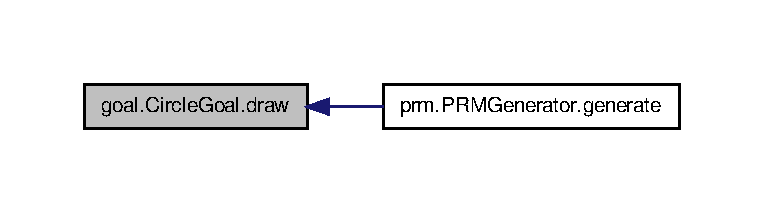
\includegraphics[width=350pt]{classgoal_1_1CircleGoal_a91dfa039728e5b68a97fbfa59f4d03e6_icgraph}
\end{center}
\end{figure}




\subsection{Member Data Documentation}
\hypertarget{classgoal_1_1CircleGoal_a2fcb77d9e22165b8d9bcde9a411d7471}{\index{goal\-::\-Circle\-Goal@{goal\-::\-Circle\-Goal}!colors@{colors}}
\index{colors@{colors}!goal::CircleGoal@{goal\-::\-Circle\-Goal}}
\subsubsection[{colors}]{\setlength{\rightskip}{0pt plus 5cm}goal.\-Circle\-Goal.\-colors}}\label{classgoal_1_1CircleGoal_a2fcb77d9e22165b8d9bcde9a411d7471}


List of colors given by Py\-Game. 



Definition at line 26 of file goal.\-py.

\hypertarget{classgoal_1_1CircleGoal_a5043cf3f8c23c20b038e44888e87622f}{\index{goal\-::\-Circle\-Goal@{goal\-::\-Circle\-Goal}!position@{position}}
\index{position@{position}!goal::CircleGoal@{goal\-::\-Circle\-Goal}}
\subsubsection[{position}]{\setlength{\rightskip}{0pt plus 5cm}goal.\-Circle\-Goal.\-position}}\label{classgoal_1_1CircleGoal_a5043cf3f8c23c20b038e44888e87622f}


The position of the circle goal. 



Definition at line 32 of file goal.\-py.

\hypertarget{classgoal_1_1CircleGoal_ab0dbe63cd28b07d45ceedf1bce771b07}{\index{goal\-::\-Circle\-Goal@{goal\-::\-Circle\-Goal}!radius@{radius}}
\index{radius@{radius}!goal::CircleGoal@{goal\-::\-Circle\-Goal}}
\subsubsection[{radius}]{\setlength{\rightskip}{0pt plus 5cm}goal.\-Circle\-Goal.\-radius}}\label{classgoal_1_1CircleGoal_ab0dbe63cd28b07d45ceedf1bce771b07}


The radius of the circle goal. 



Definition at line 29 of file goal.\-py.

\hypertarget{classgoal_1_1CircleGoal_a0868d7060d53cd1528aa699f65db3df3}{\index{goal\-::\-Circle\-Goal@{goal\-::\-Circle\-Goal}!screen@{screen}}
\index{screen@{screen}!goal::CircleGoal@{goal\-::\-Circle\-Goal}}
\subsubsection[{screen}]{\setlength{\rightskip}{0pt plus 5cm}goal.\-Circle\-Goal.\-screen}}\label{classgoal_1_1CircleGoal_a0868d7060d53cd1528aa699f65db3df3}


Py\-Game screen used to draw the circle goal. 



Definition at line 23 of file goal.\-py.



The documentation for this class was generated from the following file\-:\begin{DoxyCompactItemize}
\item 
code/\hyperlink{goal_8py}{goal.\-py}\end{DoxyCompactItemize}

\hypertarget{classconfiguration_1_1Configuration}{\section{configuration.\-Configuration Class Reference}
\label{classconfiguration_1_1Configuration}\index{configuration.\-Configuration@{configuration.\-Configuration}}
}


Static class that holds important global variables.  




Inheritance diagram for configuration.\-Configuration\-:
\nopagebreak
\begin{figure}[H]
\begin{center}
\leavevmode
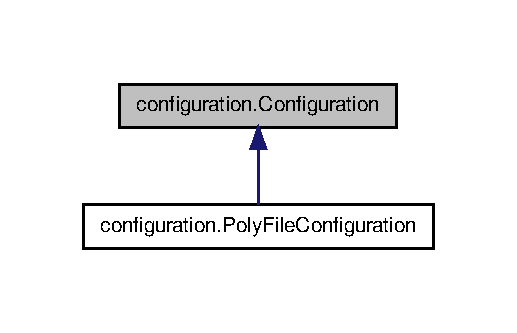
\includegraphics[width=248pt]{classconfiguration_1_1Configuration__inherit__graph}
\end{center}
\end{figure}


Collaboration diagram for configuration.\-Configuration\-:\nopagebreak
\begin{figure}[H]
\begin{center}
\leavevmode
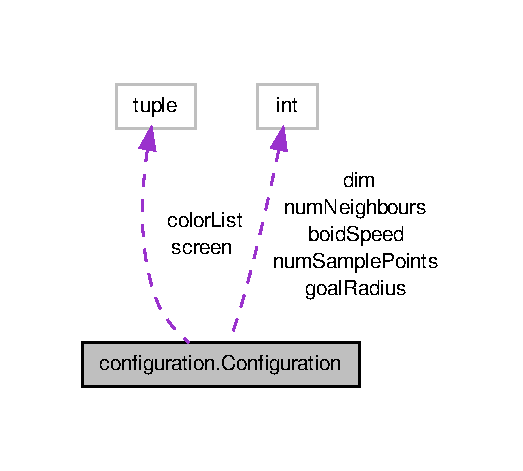
\includegraphics[width=251pt]{classconfiguration_1_1Configuration__coll__graph}
\end{center}
\end{figure}
\subsection*{Static Public Attributes}
\begin{DoxyCompactItemize}
\item 
int \hyperlink{classconfiguration_1_1Configuration_af63a65a65716f36cb11afd4d0e7f318f}{dim} = 1000
\begin{DoxyCompactList}\small\item\em Dimensions of the screen. \end{DoxyCompactList}\item 
int \hyperlink{classconfiguration_1_1Configuration_a35685f1f81ce810f4a429654c6b27334}{num\-Sample\-Points} = 300
\begin{DoxyCompactList}\small\item\em Number of sample points to use in the P\-R\-M. \end{DoxyCompactList}\item 
int \hyperlink{classconfiguration_1_1Configuration_a1a5fee18f20950a467d1b94d4d276c78}{goal\-Radius} = 20
\begin{DoxyCompactList}\small\item\em Defines the radius of all goals. \end{DoxyCompactList}\item 
int \hyperlink{classconfiguration_1_1Configuration_a5062047bc933b81cbbaa841e20cb2a67}{boid\-Speed} = 30
\begin{DoxyCompactList}\small\item\em Maximum speed of the boids. \end{DoxyCompactList}\item 
int \hyperlink{classconfiguration_1_1Configuration_a7eef6f8f2eb6d4a8fa4a45ddf9f6e1ba}{num\-Neighbours} = 3
\begin{DoxyCompactList}\small\item\em Number of neighbours the boids will influence a boid's heading. \end{DoxyCompactList}\item 
tuple \hyperlink{classconfiguration_1_1Configuration_a04b8c98906296ee65625d1472e037a75}{screen} = pygame.\-display.\-set\-\_\-mode(\hyperlink{classconfiguration_1_1Configuration_af63a65a65716f36cb11afd4d0e7f318f}{dim})
\begin{DoxyCompactList}\small\item\em The screen used to draw the simluation. \end{DoxyCompactList}\item 
tuple \hyperlink{classconfiguration_1_1Configuration_a2140643801852e373bfddf9945cf26f8}{color\-List}
\begin{DoxyCompactList}\small\item\em The list of colors (used for debugging purposes) \end{DoxyCompactList}\end{DoxyCompactItemize}


\subsection{Detailed Description}
Static class that holds important global variables. 

Definition at line 15 of file configuration.\-py.



\subsection{Member Data Documentation}
\hypertarget{classconfiguration_1_1Configuration_a5062047bc933b81cbbaa841e20cb2a67}{\index{configuration\-::\-Configuration@{configuration\-::\-Configuration}!boid\-Speed@{boid\-Speed}}
\index{boid\-Speed@{boid\-Speed}!configuration::Configuration@{configuration\-::\-Configuration}}
\subsubsection[{boid\-Speed}]{\setlength{\rightskip}{0pt plus 5cm}int configuration.\-Configuration.\-boid\-Speed = 30\hspace{0.3cm}{\ttfamily [static]}}}\label{classconfiguration_1_1Configuration_a5062047bc933b81cbbaa841e20cb2a67}


Maximum speed of the boids. 



Definition at line 27 of file configuration.\-py.

\hypertarget{classconfiguration_1_1Configuration_a2140643801852e373bfddf9945cf26f8}{\index{configuration\-::\-Configuration@{configuration\-::\-Configuration}!color\-List@{color\-List}}
\index{color\-List@{color\-List}!configuration::Configuration@{configuration\-::\-Configuration}}
\subsubsection[{color\-List}]{\setlength{\rightskip}{0pt plus 5cm}tuple configuration.\-Configuration.\-color\-List\hspace{0.3cm}{\ttfamily [static]}}}\label{classconfiguration_1_1Configuration_a2140643801852e373bfddf9945cf26f8}
{\bfseries Initial value\-:}
\begin{DoxyCode}
1 = map(
2         \textcolor{keyword}{lambda} k: color.THECOLORS[k], 
3         color.THECOLORS.keys()
4     )
\end{DoxyCode}


The list of colors (used for debugging purposes) 



Definition at line 37 of file configuration.\-py.

\hypertarget{classconfiguration_1_1Configuration_af63a65a65716f36cb11afd4d0e7f318f}{\index{configuration\-::\-Configuration@{configuration\-::\-Configuration}!dim@{dim}}
\index{dim@{dim}!configuration::Configuration@{configuration\-::\-Configuration}}
\subsubsection[{dim}]{\setlength{\rightskip}{0pt plus 5cm}int configuration.\-Configuration.\-dim = 1000\hspace{0.3cm}{\ttfamily [static]}}}\label{classconfiguration_1_1Configuration_af63a65a65716f36cb11afd4d0e7f318f}


Dimensions of the screen. 



Definition at line 18 of file configuration.\-py.

\hypertarget{classconfiguration_1_1Configuration_a1a5fee18f20950a467d1b94d4d276c78}{\index{configuration\-::\-Configuration@{configuration\-::\-Configuration}!goal\-Radius@{goal\-Radius}}
\index{goal\-Radius@{goal\-Radius}!configuration::Configuration@{configuration\-::\-Configuration}}
\subsubsection[{goal\-Radius}]{\setlength{\rightskip}{0pt plus 5cm}int configuration.\-Configuration.\-goal\-Radius = 20\hspace{0.3cm}{\ttfamily [static]}}}\label{classconfiguration_1_1Configuration_a1a5fee18f20950a467d1b94d4d276c78}


Defines the radius of all goals. 



Definition at line 24 of file configuration.\-py.

\hypertarget{classconfiguration_1_1Configuration_a7eef6f8f2eb6d4a8fa4a45ddf9f6e1ba}{\index{configuration\-::\-Configuration@{configuration\-::\-Configuration}!num\-Neighbours@{num\-Neighbours}}
\index{num\-Neighbours@{num\-Neighbours}!configuration::Configuration@{configuration\-::\-Configuration}}
\subsubsection[{num\-Neighbours}]{\setlength{\rightskip}{0pt plus 5cm}int configuration.\-Configuration.\-num\-Neighbours = 3\hspace{0.3cm}{\ttfamily [static]}}}\label{classconfiguration_1_1Configuration_a7eef6f8f2eb6d4a8fa4a45ddf9f6e1ba}


Number of neighbours the boids will influence a boid's heading. 



Definition at line 31 of file configuration.\-py.

\hypertarget{classconfiguration_1_1Configuration_a35685f1f81ce810f4a429654c6b27334}{\index{configuration\-::\-Configuration@{configuration\-::\-Configuration}!num\-Sample\-Points@{num\-Sample\-Points}}
\index{num\-Sample\-Points@{num\-Sample\-Points}!configuration::Configuration@{configuration\-::\-Configuration}}
\subsubsection[{num\-Sample\-Points}]{\setlength{\rightskip}{0pt plus 5cm}int configuration.\-Configuration.\-num\-Sample\-Points = 300\hspace{0.3cm}{\ttfamily [static]}}}\label{classconfiguration_1_1Configuration_a35685f1f81ce810f4a429654c6b27334}


Number of sample points to use in the P\-R\-M. 



Definition at line 21 of file configuration.\-py.

\hypertarget{classconfiguration_1_1Configuration_a04b8c98906296ee65625d1472e037a75}{\index{configuration\-::\-Configuration@{configuration\-::\-Configuration}!screen@{screen}}
\index{screen@{screen}!configuration::Configuration@{configuration\-::\-Configuration}}
\subsubsection[{screen}]{\setlength{\rightskip}{0pt plus 5cm}tuple configuration.\-Configuration.\-screen = pygame.\-display.\-set\-\_\-mode({\bf dim})\hspace{0.3cm}{\ttfamily [static]}}}\label{classconfiguration_1_1Configuration_a04b8c98906296ee65625d1472e037a75}


The screen used to draw the simluation. 



Definition at line 34 of file configuration.\-py.



The documentation for this class was generated from the following file\-:\begin{DoxyCompactItemize}
\item 
code/\hyperlink{configuration_8py}{configuration.\-py}\end{DoxyCompactItemize}

\hypertarget{classdict}{\section{dict Class Reference}
\label{classdict}\index{dict@{dict}}
}


Inheritance diagram for dict\-:\nopagebreak
\begin{figure}[H]
\begin{center}
\leavevmode
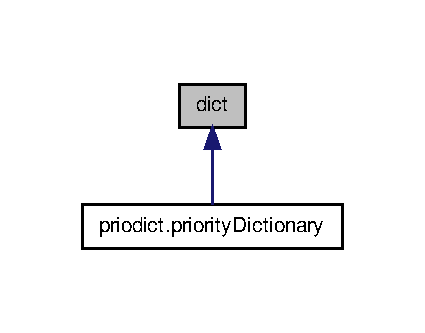
\includegraphics[width=204pt]{classdict__inherit__graph}
\end{center}
\end{figure}


The documentation for this class was generated from the following file\-:\begin{DoxyCompactItemize}
\item 
code/\hyperlink{priodict_8py}{priodict.\-py (\-Concurrent Versions System (\-C\-V\-S) 1.\-12.\-13-\/\-Mir\-Debian-\/9 (client/server))}\end{DoxyCompactItemize}

\hypertarget{classboidsimulation_1_1FlockSim}{\section{boidsimulation.\-Flock\-Sim Class Reference}
\label{classboidsimulation_1_1FlockSim}\index{boidsimulation.\-Flock\-Sim@{boidsimulation.\-Flock\-Sim}}
}


Main class for that is used for the simulation and display of the flock.  


\subsection*{Public Member Functions}
\begin{DoxyCompactItemize}
\item 
def \hyperlink{classboidsimulation_1_1FlockSim_a7221a17466a06ad9018024d80b6bbff8}{\-\_\-\-\_\-init\-\_\-\-\_\-}
\begin{DoxyCompactList}\small\item\em Initializes the flock and the display mechanism (Py\-Game) \end{DoxyCompactList}\item 
def \hyperlink{classboidsimulation_1_1FlockSim_ad69cb572160cb83e3c868fc9de4a9e75}{avg}
\begin{DoxyCompactList}\small\item\em Gets the average of a list. \end{DoxyCompactList}\item 
def \hyperlink{classboidsimulation_1_1FlockSim_ae638beb355d9d953fe51e087ff1e6e94}{get\-Stats}
\begin{DoxyCompactList}\small\item\em Gets runtime statistics about the simulation and writes it to a file. \end{DoxyCompactList}\item 
def \hyperlink{classboidsimulation_1_1FlockSim_a57c1ef2f27ac7157afdabae4eefcc370}{get\-Boid\-Data}
\begin{DoxyCompactList}\small\item\em Writes all of the boid positions to a file. \end{DoxyCompactList}\item 
def \hyperlink{classboidsimulation_1_1FlockSim_a4fb29f4acff12a3d9b9a88280501320d}{animate}
\begin{DoxyCompactList}\small\item\em Renders and then allows interactive playback of the swarm simulation data. \end{DoxyCompactList}\item 
def \hyperlink{classboidsimulation_1_1FlockSim_a86097d942af27dc5df9f7190befd363c}{init\-\_\-prm}
\begin{DoxyCompactList}\small\item\em Initializes the P\-R\-M generator used for the global planner. \end{DoxyCompactList}\item 
def \hyperlink{classboidsimulation_1_1FlockSim_a3c456990ff58b2a5dfae2dd2b5b6d294}{render}
\begin{DoxyCompactList}\small\item\em Renders the scene. \end{DoxyCompactList}\item 
def \hyperlink{classboidsimulation_1_1FlockSim_a50ded4dc206f7ae1011347ef234a0091}{play}
\begin{DoxyCompactList}\small\item\em Plays the scene after it has rendered. \end{DoxyCompactList}\end{DoxyCompactItemize}
\subsection*{Public Attributes}
\begin{DoxyCompactItemize}
\item 
\hyperlink{classboidsimulation_1_1FlockSim_a970e9fcbc5d69b3987f226af5249038a}{done}
\begin{DoxyCompactList}\small\item\em Tells if the flock has reached the end goal (used again to see if the escape or space bar were hit to stop the rendering) \end{DoxyCompactList}\item 
\hyperlink{classboidsimulation_1_1FlockSim_ac9c61aa93f3db94b9a340b8555d90adf}{B\-L\-A\-C\-K}
\begin{DoxyCompactList}\small\item\em Defines the color black. \end{DoxyCompactList}\item 
\hyperlink{classboidsimulation_1_1FlockSim_afe8d83a914aeae9d188cdf61053de56c}{W\-H\-I\-T\-E}
\begin{DoxyCompactList}\small\item\em Defines the color white. \end{DoxyCompactList}\item 
\hyperlink{classboidsimulation_1_1FlockSim_aa5993f8033dcbbb0383c204877d1dd20}{font}
\begin{DoxyCompactList}\small\item\em The font that is used for displaying the frame number. \end{DoxyCompactList}\item 
\hyperlink{classboidsimulation_1_1FlockSim_a2ba5ffd4d4ef009af8735d838eaf59d3}{dim}
\begin{DoxyCompactList}\small\item\em The dimensions of the Py\-Game screen. \end{DoxyCompactList}\item 
\hyperlink{classboidsimulation_1_1FlockSim_abf487d6e84851334a79656b5df3c8492}{config}
\begin{DoxyCompactList}\small\item\em The configuration object (in this case the configuration is defined by an exterior file) \end{DoxyCompactList}\item 
\hyperlink{classboidsimulation_1_1FlockSim_a1658c675990b8bdb3955cae1b7292b38}{s\-Pos}
\begin{DoxyCompactList}\small\item\em The starting point of the flock. \end{DoxyCompactList}\item 
\hyperlink{classboidsimulation_1_1FlockSim_acb064f74364917a97ca9d3accdf96f45}{e\-Pos}
\begin{DoxyCompactList}\small\item\em The position of the last goal for the flock. \end{DoxyCompactList}\item 
\hyperlink{classboidsimulation_1_1FlockSim_a60f47dc6f8186030cd22f3ca3b37c4e6}{surface\-List}
\begin{DoxyCompactList}\small\item\em Variable used to store the list of surfaces for simulation playback. \end{DoxyCompactList}\item 
\hyperlink{classboidsimulation_1_1FlockSim_a1febd4cacbdcffb5b9d096d4716af78f}{iterations}
\begin{DoxyCompactList}\small\item\em Maximum number of iterations. \end{DoxyCompactList}\item 
\hyperlink{classboidsimulation_1_1FlockSim_a7daba8b4e771dcd6f6a7357bda59c56a}{frame\-Counter}
\begin{DoxyCompactList}\small\item\em Counts which frame the user is on for the playback (don't know why it it is set to -\/2, it just works) \end{DoxyCompactList}\item 
\hyperlink{classboidsimulation_1_1FlockSim_af378fd310919691dec50f5d312931726}{counter}
\begin{DoxyCompactList}\small\item\em Global counter used for the rendering and the playback. \end{DoxyCompactList}\item 
\hyperlink{classboidsimulation_1_1FlockSim_a125fa6c2909527f18c768f09606ab442}{flock\-Size}
\begin{DoxyCompactList}\small\item\em The size of the flock (number of boids) \end{DoxyCompactList}\item 
\hyperlink{classboidsimulation_1_1FlockSim_a50b375f7caa0e33d87141d2cde14526f}{map\-File}
\begin{DoxyCompactList}\small\item\em The file that contains the data about the obstacles. \end{DoxyCompactList}\item 
\hyperlink{classboidsimulation_1_1FlockSim_a96885e067ac2333f807eaa9580a2ece4}{data\-File}
\begin{DoxyCompactList}\small\item\em The file that the statistics data will be written to. \end{DoxyCompactList}\item 
\hyperlink{classboidsimulation_1_1FlockSim_aea78473e0e592e48b6047f49f8254cc1}{start\-Time}
\item 
\hyperlink{classboidsimulation_1_1FlockSim_ae60982002b6c8c922b3822dbdec4bd41}{num\-In\-Goal}
\end{DoxyCompactItemize}


\subsection{Detailed Description}
Main class for that is used for the simulation and display of the flock. 

It also is used to gather statistics about the flock and present them in a useful manner. 

Definition at line 20 of file boidsimulation.\-py.



\subsection{Constructor \& Destructor Documentation}
\hypertarget{classboidsimulation_1_1FlockSim_a7221a17466a06ad9018024d80b6bbff8}{\index{boidsimulation\-::\-Flock\-Sim@{boidsimulation\-::\-Flock\-Sim}!\-\_\-\-\_\-init\-\_\-\-\_\-@{\-\_\-\-\_\-init\-\_\-\-\_\-}}
\index{\-\_\-\-\_\-init\-\_\-\-\_\-@{\-\_\-\-\_\-init\-\_\-\-\_\-}!boidsimulation::FlockSim@{boidsimulation\-::\-Flock\-Sim}}
\subsubsection[{\-\_\-\-\_\-init\-\_\-\-\_\-}]{\setlength{\rightskip}{0pt plus 5cm}def boidsimulation.\-Flock\-Sim.\-\_\-\-\_\-init\-\_\-\-\_\- (
\begin{DoxyParamCaption}
\item[{}]{self, }
\item[{}]{flock\-Size, }
\item[{}]{start\-Point, }
\item[{}]{end\-Point, }
\item[{}]{\-\_\-map\-File = {\ttfamily None}, }
\item[{}]{\-\_\-data\-File = {\ttfamily None}}
\end{DoxyParamCaption}
)}}\label{classboidsimulation_1_1FlockSim_a7221a17466a06ad9018024d80b6bbff8}


Initializes the flock and the display mechanism (Py\-Game) 


\begin{DoxyParams}{Parameters}
{\em flock\-Size} & The size of the flock (number of boids) \\
\hline
{\em start\-Point} & The macro starting position of the flock \\
\hline
{\em end\-Point} & The last goal point for the flock \\
\hline
{\em \-\_\-map\-File} & The file containing details about the obstacles \\
\hline
{\em \-\_\-data\-File} & The file that the data will be exported to \\
\hline
\end{DoxyParams}


Definition at line 30 of file boidsimulation.\-py.



\subsection{Member Function Documentation}
\hypertarget{classboidsimulation_1_1FlockSim_a4fb29f4acff12a3d9b9a88280501320d}{\index{boidsimulation\-::\-Flock\-Sim@{boidsimulation\-::\-Flock\-Sim}!animate@{animate}}
\index{animate@{animate}!boidsimulation::FlockSim@{boidsimulation\-::\-Flock\-Sim}}
\subsubsection[{animate}]{\setlength{\rightskip}{0pt plus 5cm}def boidsimulation.\-Flock\-Sim.\-animate (
\begin{DoxyParamCaption}
\item[{}]{self}
\end{DoxyParamCaption}
)}}\label{classboidsimulation_1_1FlockSim_a4fb29f4acff12a3d9b9a88280501320d}


Renders and then allows interactive playback of the swarm simulation data. 



Definition at line 137 of file boidsimulation.\-py.



Here is the call graph for this function\-:\nopagebreak
\begin{figure}[H]
\begin{center}
\leavevmode
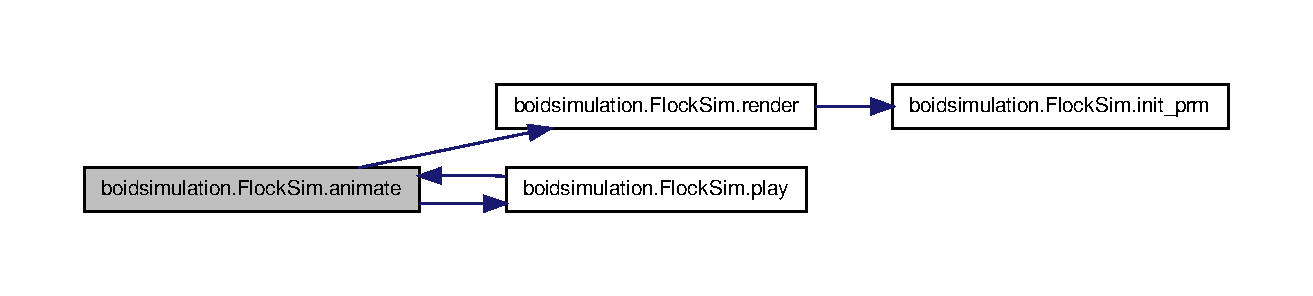
\includegraphics[width=350pt]{classboidsimulation_1_1FlockSim_a4fb29f4acff12a3d9b9a88280501320d_cgraph}
\end{center}
\end{figure}




Here is the caller graph for this function\-:\nopagebreak
\begin{figure}[H]
\begin{center}
\leavevmode
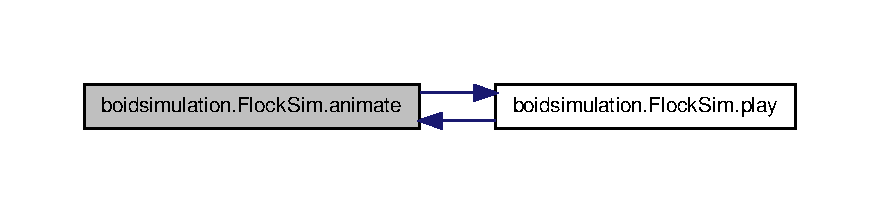
\includegraphics[width=350pt]{classboidsimulation_1_1FlockSim_a4fb29f4acff12a3d9b9a88280501320d_icgraph}
\end{center}
\end{figure}


\hypertarget{classboidsimulation_1_1FlockSim_ad69cb572160cb83e3c868fc9de4a9e75}{\index{boidsimulation\-::\-Flock\-Sim@{boidsimulation\-::\-Flock\-Sim}!avg@{avg}}
\index{avg@{avg}!boidsimulation::FlockSim@{boidsimulation\-::\-Flock\-Sim}}
\subsubsection[{avg}]{\setlength{\rightskip}{0pt plus 5cm}def boidsimulation.\-Flock\-Sim.\-avg (
\begin{DoxyParamCaption}
\item[{}]{self, }
\item[{}]{l}
\end{DoxyParamCaption}
)}}\label{classboidsimulation_1_1FlockSim_ad69cb572160cb83e3c868fc9de4a9e75}


Gets the average of a list. 


\begin{DoxyParams}{Parameters}
{\em l} & The list to be averaged \\
\hline
\end{DoxyParams}
\begin{DoxyReturn}{Returns}
l The average value in list l 
\end{DoxyReturn}


Definition at line 87 of file boidsimulation.\-py.



Here is the caller graph for this function\-:\nopagebreak
\begin{figure}[H]
\begin{center}
\leavevmode
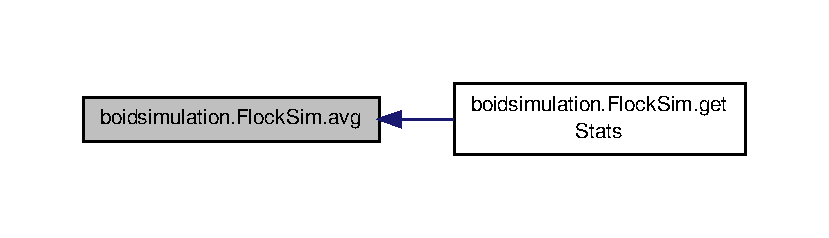
\includegraphics[width=350pt]{classboidsimulation_1_1FlockSim_ad69cb572160cb83e3c868fc9de4a9e75_icgraph}
\end{center}
\end{figure}


\hypertarget{classboidsimulation_1_1FlockSim_a57c1ef2f27ac7157afdabae4eefcc370}{\index{boidsimulation\-::\-Flock\-Sim@{boidsimulation\-::\-Flock\-Sim}!get\-Boid\-Data@{get\-Boid\-Data}}
\index{get\-Boid\-Data@{get\-Boid\-Data}!boidsimulation::FlockSim@{boidsimulation\-::\-Flock\-Sim}}
\subsubsection[{get\-Boid\-Data}]{\setlength{\rightskip}{0pt plus 5cm}def boidsimulation.\-Flock\-Sim.\-get\-Boid\-Data (
\begin{DoxyParamCaption}
\item[{}]{self}
\end{DoxyParamCaption}
)}}\label{classboidsimulation_1_1FlockSim_a57c1ef2f27ac7157afdabae4eefcc370}


Writes all of the boid positions to a file. 



Definition at line 126 of file boidsimulation.\-py.

\hypertarget{classboidsimulation_1_1FlockSim_ae638beb355d9d953fe51e087ff1e6e94}{\index{boidsimulation\-::\-Flock\-Sim@{boidsimulation\-::\-Flock\-Sim}!get\-Stats@{get\-Stats}}
\index{get\-Stats@{get\-Stats}!boidsimulation::FlockSim@{boidsimulation\-::\-Flock\-Sim}}
\subsubsection[{get\-Stats}]{\setlength{\rightskip}{0pt plus 5cm}def boidsimulation.\-Flock\-Sim.\-get\-Stats (
\begin{DoxyParamCaption}
\item[{}]{self}
\end{DoxyParamCaption}
)}}\label{classboidsimulation_1_1FlockSim_ae638beb355d9d953fe51e087ff1e6e94}


Gets runtime statistics about the simulation and writes it to a file. 

Currently, the statistics being gathered are the current time that has passed, the average distance between the boids, the average minimum distance between the boids, and the number of boids that have finished 

Definition at line 100 of file boidsimulation.\-py.



Here is the call graph for this function\-:\nopagebreak
\begin{figure}[H]
\begin{center}
\leavevmode
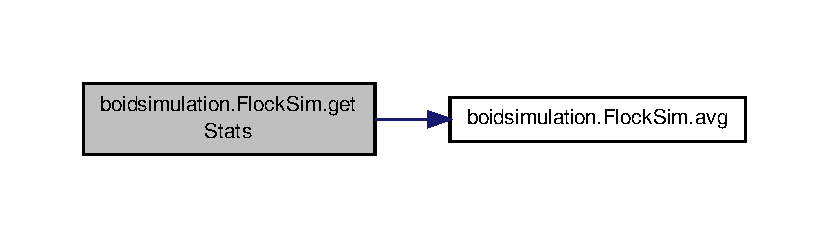
\includegraphics[width=350pt]{classboidsimulation_1_1FlockSim_ae638beb355d9d953fe51e087ff1e6e94_cgraph}
\end{center}
\end{figure}


\hypertarget{classboidsimulation_1_1FlockSim_a86097d942af27dc5df9f7190befd363c}{\index{boidsimulation\-::\-Flock\-Sim@{boidsimulation\-::\-Flock\-Sim}!init\-\_\-prm@{init\-\_\-prm}}
\index{init\-\_\-prm@{init\-\_\-prm}!boidsimulation::FlockSim@{boidsimulation\-::\-Flock\-Sim}}
\subsubsection[{init\-\_\-prm}]{\setlength{\rightskip}{0pt plus 5cm}def boidsimulation.\-Flock\-Sim.\-init\-\_\-prm (
\begin{DoxyParamCaption}
\item[{}]{self}
\end{DoxyParamCaption}
)}}\label{classboidsimulation_1_1FlockSim_a86097d942af27dc5df9f7190befd363c}


Initializes the P\-R\-M generator used for the global planner. 

Also sets the boid list for the rest of the flock 

Definition at line 146 of file boidsimulation.\-py.



Here is the caller graph for this function\-:\nopagebreak
\begin{figure}[H]
\begin{center}
\leavevmode
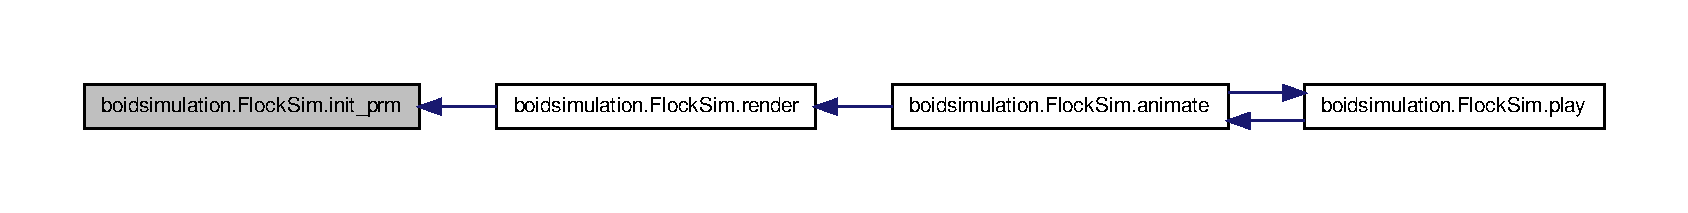
\includegraphics[width=350pt]{classboidsimulation_1_1FlockSim_a86097d942af27dc5df9f7190befd363c_icgraph}
\end{center}
\end{figure}


\hypertarget{classboidsimulation_1_1FlockSim_a50ded4dc206f7ae1011347ef234a0091}{\index{boidsimulation\-::\-Flock\-Sim@{boidsimulation\-::\-Flock\-Sim}!play@{play}}
\index{play@{play}!boidsimulation::FlockSim@{boidsimulation\-::\-Flock\-Sim}}
\subsubsection[{play}]{\setlength{\rightskip}{0pt plus 5cm}def boidsimulation.\-Flock\-Sim.\-play (
\begin{DoxyParamCaption}
\item[{}]{self}
\end{DoxyParamCaption}
)}}\label{classboidsimulation_1_1FlockSim_a50ded4dc206f7ae1011347ef234a0091}


Plays the scene after it has rendered. 

Iterates through surfaces that have been stored in surface\-List and blits the new surface on the screen 

Definition at line 212 of file boidsimulation.\-py.



Here is the call graph for this function\-:\nopagebreak
\begin{figure}[H]
\begin{center}
\leavevmode
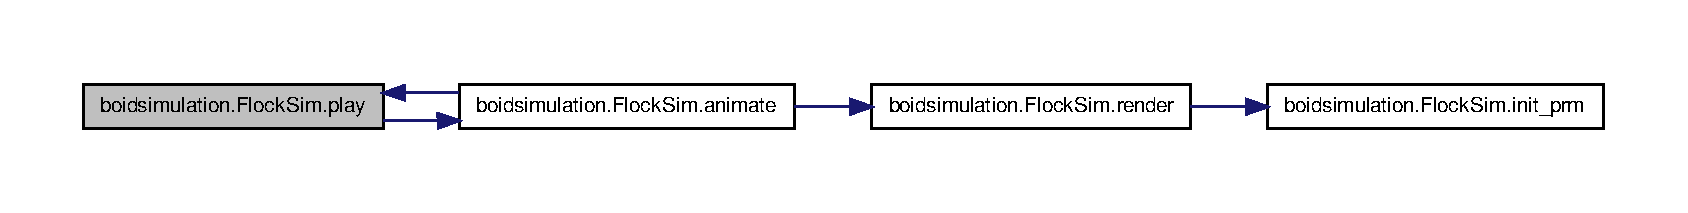
\includegraphics[width=350pt]{classboidsimulation_1_1FlockSim_a50ded4dc206f7ae1011347ef234a0091_cgraph}
\end{center}
\end{figure}




Here is the caller graph for this function\-:\nopagebreak
\begin{figure}[H]
\begin{center}
\leavevmode
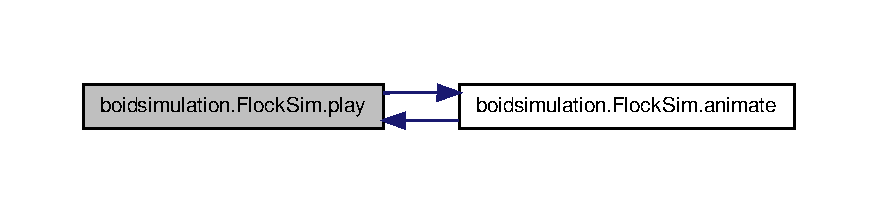
\includegraphics[width=350pt]{classboidsimulation_1_1FlockSim_a50ded4dc206f7ae1011347ef234a0091_icgraph}
\end{center}
\end{figure}


\hypertarget{classboidsimulation_1_1FlockSim_a3c456990ff58b2a5dfae2dd2b5b6d294}{\index{boidsimulation\-::\-Flock\-Sim@{boidsimulation\-::\-Flock\-Sim}!render@{render}}
\index{render@{render}!boidsimulation::FlockSim@{boidsimulation\-::\-Flock\-Sim}}
\subsubsection[{render}]{\setlength{\rightskip}{0pt plus 5cm}def boidsimulation.\-Flock\-Sim.\-render (
\begin{DoxyParamCaption}
\item[{}]{self, }
\item[{}]{for\-Play = {\ttfamily False}}
\end{DoxyParamCaption}
)}}\label{classboidsimulation_1_1FlockSim_a3c456990ff58b2a5dfae2dd2b5b6d294}


Renders the scene. 

This means that the time taken for the boids to reach the goal in this function is that actual amount of computational time needed. 
\begin{DoxyParams}{Parameters}
{\em for\-Play} & Specifies if the surface data should be recorded for animation \\
\hline
\end{DoxyParams}


Definition at line 167 of file boidsimulation.\-py.



Here is the call graph for this function\-:\nopagebreak
\begin{figure}[H]
\begin{center}
\leavevmode
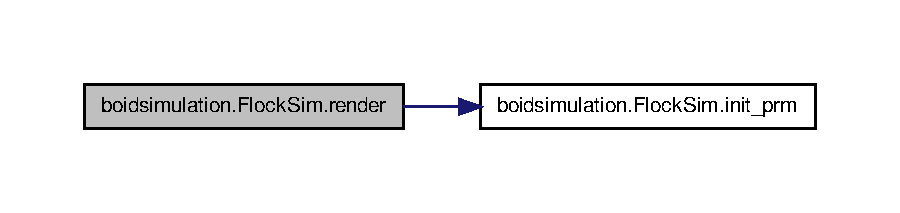
\includegraphics[width=350pt]{classboidsimulation_1_1FlockSim_a3c456990ff58b2a5dfae2dd2b5b6d294_cgraph}
\end{center}
\end{figure}




Here is the caller graph for this function\-:\nopagebreak
\begin{figure}[H]
\begin{center}
\leavevmode
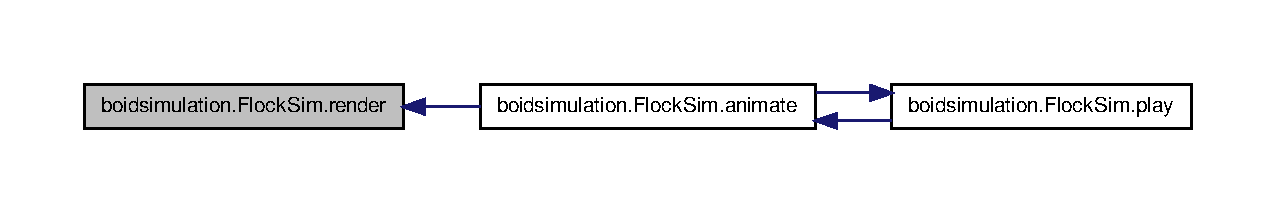
\includegraphics[width=350pt]{classboidsimulation_1_1FlockSim_a3c456990ff58b2a5dfae2dd2b5b6d294_icgraph}
\end{center}
\end{figure}




\subsection{Member Data Documentation}
\hypertarget{classboidsimulation_1_1FlockSim_ac9c61aa93f3db94b9a340b8555d90adf}{\index{boidsimulation\-::\-Flock\-Sim@{boidsimulation\-::\-Flock\-Sim}!B\-L\-A\-C\-K@{B\-L\-A\-C\-K}}
\index{B\-L\-A\-C\-K@{B\-L\-A\-C\-K}!boidsimulation::FlockSim@{boidsimulation\-::\-Flock\-Sim}}
\subsubsection[{B\-L\-A\-C\-K}]{\setlength{\rightskip}{0pt plus 5cm}boidsimulation.\-Flock\-Sim.\-B\-L\-A\-C\-K}}\label{classboidsimulation_1_1FlockSim_ac9c61aa93f3db94b9a340b8555d90adf}


Defines the color black. 



Definition at line 38 of file boidsimulation.\-py.

\hypertarget{classboidsimulation_1_1FlockSim_abf487d6e84851334a79656b5df3c8492}{\index{boidsimulation\-::\-Flock\-Sim@{boidsimulation\-::\-Flock\-Sim}!config@{config}}
\index{config@{config}!boidsimulation::FlockSim@{boidsimulation\-::\-Flock\-Sim}}
\subsubsection[{config}]{\setlength{\rightskip}{0pt plus 5cm}boidsimulation.\-Flock\-Sim.\-config}}\label{classboidsimulation_1_1FlockSim_abf487d6e84851334a79656b5df3c8492}


The configuration object (in this case the configuration is defined by an exterior file) 



Definition at line 51 of file boidsimulation.\-py.

\hypertarget{classboidsimulation_1_1FlockSim_af378fd310919691dec50f5d312931726}{\index{boidsimulation\-::\-Flock\-Sim@{boidsimulation\-::\-Flock\-Sim}!counter@{counter}}
\index{counter@{counter}!boidsimulation::FlockSim@{boidsimulation\-::\-Flock\-Sim}}
\subsubsection[{counter}]{\setlength{\rightskip}{0pt plus 5cm}boidsimulation.\-Flock\-Sim.\-counter}}\label{classboidsimulation_1_1FlockSim_af378fd310919691dec50f5d312931726}


Global counter used for the rendering and the playback. 



Definition at line 70 of file boidsimulation.\-py.

\hypertarget{classboidsimulation_1_1FlockSim_a96885e067ac2333f807eaa9580a2ece4}{\index{boidsimulation\-::\-Flock\-Sim@{boidsimulation\-::\-Flock\-Sim}!data\-File@{data\-File}}
\index{data\-File@{data\-File}!boidsimulation::FlockSim@{boidsimulation\-::\-Flock\-Sim}}
\subsubsection[{data\-File}]{\setlength{\rightskip}{0pt plus 5cm}boidsimulation.\-Flock\-Sim.\-data\-File}}\label{classboidsimulation_1_1FlockSim_a96885e067ac2333f807eaa9580a2ece4}


The file that the statistics data will be written to. 



Definition at line 79 of file boidsimulation.\-py.

\hypertarget{classboidsimulation_1_1FlockSim_a2ba5ffd4d4ef009af8735d838eaf59d3}{\index{boidsimulation\-::\-Flock\-Sim@{boidsimulation\-::\-Flock\-Sim}!dim@{dim}}
\index{dim@{dim}!boidsimulation::FlockSim@{boidsimulation\-::\-Flock\-Sim}}
\subsubsection[{dim}]{\setlength{\rightskip}{0pt plus 5cm}boidsimulation.\-Flock\-Sim.\-dim}}\label{classboidsimulation_1_1FlockSim_a2ba5ffd4d4ef009af8735d838eaf59d3}


The dimensions of the Py\-Game screen. 



Definition at line 47 of file boidsimulation.\-py.

\hypertarget{classboidsimulation_1_1FlockSim_a970e9fcbc5d69b3987f226af5249038a}{\index{boidsimulation\-::\-Flock\-Sim@{boidsimulation\-::\-Flock\-Sim}!done@{done}}
\index{done@{done}!boidsimulation::FlockSim@{boidsimulation\-::\-Flock\-Sim}}
\subsubsection[{done}]{\setlength{\rightskip}{0pt plus 5cm}boidsimulation.\-Flock\-Sim.\-done}}\label{classboidsimulation_1_1FlockSim_a970e9fcbc5d69b3987f226af5249038a}


Tells if the flock has reached the end goal (used again to see if the escape or space bar were hit to stop the rendering) 



Definition at line 35 of file boidsimulation.\-py.

\hypertarget{classboidsimulation_1_1FlockSim_acb064f74364917a97ca9d3accdf96f45}{\index{boidsimulation\-::\-Flock\-Sim@{boidsimulation\-::\-Flock\-Sim}!e\-Pos@{e\-Pos}}
\index{e\-Pos@{e\-Pos}!boidsimulation::FlockSim@{boidsimulation\-::\-Flock\-Sim}}
\subsubsection[{e\-Pos}]{\setlength{\rightskip}{0pt plus 5cm}boidsimulation.\-Flock\-Sim.\-e\-Pos}}\label{classboidsimulation_1_1FlockSim_acb064f74364917a97ca9d3accdf96f45}


The position of the last goal for the flock. 



Definition at line 57 of file boidsimulation.\-py.

\hypertarget{classboidsimulation_1_1FlockSim_a125fa6c2909527f18c768f09606ab442}{\index{boidsimulation\-::\-Flock\-Sim@{boidsimulation\-::\-Flock\-Sim}!flock\-Size@{flock\-Size}}
\index{flock\-Size@{flock\-Size}!boidsimulation::FlockSim@{boidsimulation\-::\-Flock\-Sim}}
\subsubsection[{flock\-Size}]{\setlength{\rightskip}{0pt plus 5cm}boidsimulation.\-Flock\-Sim.\-flock\-Size}}\label{classboidsimulation_1_1FlockSim_a125fa6c2909527f18c768f09606ab442}


The size of the flock (number of boids) 



Definition at line 73 of file boidsimulation.\-py.

\hypertarget{classboidsimulation_1_1FlockSim_aa5993f8033dcbbb0383c204877d1dd20}{\index{boidsimulation\-::\-Flock\-Sim@{boidsimulation\-::\-Flock\-Sim}!font@{font}}
\index{font@{font}!boidsimulation::FlockSim@{boidsimulation\-::\-Flock\-Sim}}
\subsubsection[{font}]{\setlength{\rightskip}{0pt plus 5cm}boidsimulation.\-Flock\-Sim.\-font}}\label{classboidsimulation_1_1FlockSim_aa5993f8033dcbbb0383c204877d1dd20}


The font that is used for displaying the frame number. 



Definition at line 44 of file boidsimulation.\-py.

\hypertarget{classboidsimulation_1_1FlockSim_a7daba8b4e771dcd6f6a7357bda59c56a}{\index{boidsimulation\-::\-Flock\-Sim@{boidsimulation\-::\-Flock\-Sim}!frame\-Counter@{frame\-Counter}}
\index{frame\-Counter@{frame\-Counter}!boidsimulation::FlockSim@{boidsimulation\-::\-Flock\-Sim}}
\subsubsection[{frame\-Counter}]{\setlength{\rightskip}{0pt plus 5cm}boidsimulation.\-Flock\-Sim.\-frame\-Counter}}\label{classboidsimulation_1_1FlockSim_a7daba8b4e771dcd6f6a7357bda59c56a}


Counts which frame the user is on for the playback (don't know why it it is set to -\/2, it just works) 



Definition at line 67 of file boidsimulation.\-py.

\hypertarget{classboidsimulation_1_1FlockSim_a1febd4cacbdcffb5b9d096d4716af78f}{\index{boidsimulation\-::\-Flock\-Sim@{boidsimulation\-::\-Flock\-Sim}!iterations@{iterations}}
\index{iterations@{iterations}!boidsimulation::FlockSim@{boidsimulation\-::\-Flock\-Sim}}
\subsubsection[{iterations}]{\setlength{\rightskip}{0pt plus 5cm}boidsimulation.\-Flock\-Sim.\-iterations}}\label{classboidsimulation_1_1FlockSim_a1febd4cacbdcffb5b9d096d4716af78f}


Maximum number of iterations. 



Definition at line 63 of file boidsimulation.\-py.

\hypertarget{classboidsimulation_1_1FlockSim_a50b375f7caa0e33d87141d2cde14526f}{\index{boidsimulation\-::\-Flock\-Sim@{boidsimulation\-::\-Flock\-Sim}!map\-File@{map\-File}}
\index{map\-File@{map\-File}!boidsimulation::FlockSim@{boidsimulation\-::\-Flock\-Sim}}
\subsubsection[{map\-File}]{\setlength{\rightskip}{0pt plus 5cm}boidsimulation.\-Flock\-Sim.\-map\-File}}\label{classboidsimulation_1_1FlockSim_a50b375f7caa0e33d87141d2cde14526f}


The file that contains the data about the obstacles. 



Definition at line 76 of file boidsimulation.\-py.

\hypertarget{classboidsimulation_1_1FlockSim_ae60982002b6c8c922b3822dbdec4bd41}{\index{boidsimulation\-::\-Flock\-Sim@{boidsimulation\-::\-Flock\-Sim}!num\-In\-Goal@{num\-In\-Goal}}
\index{num\-In\-Goal@{num\-In\-Goal}!boidsimulation::FlockSim@{boidsimulation\-::\-Flock\-Sim}}
\subsubsection[{num\-In\-Goal}]{\setlength{\rightskip}{0pt plus 5cm}boidsimulation.\-Flock\-Sim.\-num\-In\-Goal}}\label{classboidsimulation_1_1FlockSim_ae60982002b6c8c922b3822dbdec4bd41}


Definition at line 181 of file boidsimulation.\-py.

\hypertarget{classboidsimulation_1_1FlockSim_a1658c675990b8bdb3955cae1b7292b38}{\index{boidsimulation\-::\-Flock\-Sim@{boidsimulation\-::\-Flock\-Sim}!s\-Pos@{s\-Pos}}
\index{s\-Pos@{s\-Pos}!boidsimulation::FlockSim@{boidsimulation\-::\-Flock\-Sim}}
\subsubsection[{s\-Pos}]{\setlength{\rightskip}{0pt plus 5cm}boidsimulation.\-Flock\-Sim.\-s\-Pos}}\label{classboidsimulation_1_1FlockSim_a1658c675990b8bdb3955cae1b7292b38}


The starting point of the flock. 



Definition at line 54 of file boidsimulation.\-py.

\hypertarget{classboidsimulation_1_1FlockSim_aea78473e0e592e48b6047f49f8254cc1}{\index{boidsimulation\-::\-Flock\-Sim@{boidsimulation\-::\-Flock\-Sim}!start\-Time@{start\-Time}}
\index{start\-Time@{start\-Time}!boidsimulation::FlockSim@{boidsimulation\-::\-Flock\-Sim}}
\subsubsection[{start\-Time}]{\setlength{\rightskip}{0pt plus 5cm}boidsimulation.\-Flock\-Sim.\-start\-Time}}\label{classboidsimulation_1_1FlockSim_aea78473e0e592e48b6047f49f8254cc1}


Definition at line 171 of file boidsimulation.\-py.

\hypertarget{classboidsimulation_1_1FlockSim_a60f47dc6f8186030cd22f3ca3b37c4e6}{\index{boidsimulation\-::\-Flock\-Sim@{boidsimulation\-::\-Flock\-Sim}!surface\-List@{surface\-List}}
\index{surface\-List@{surface\-List}!boidsimulation::FlockSim@{boidsimulation\-::\-Flock\-Sim}}
\subsubsection[{surface\-List}]{\setlength{\rightskip}{0pt plus 5cm}boidsimulation.\-Flock\-Sim.\-surface\-List}}\label{classboidsimulation_1_1FlockSim_a60f47dc6f8186030cd22f3ca3b37c4e6}


Variable used to store the list of surfaces for simulation playback. 



Definition at line 60 of file boidsimulation.\-py.

\hypertarget{classboidsimulation_1_1FlockSim_afe8d83a914aeae9d188cdf61053de56c}{\index{boidsimulation\-::\-Flock\-Sim@{boidsimulation\-::\-Flock\-Sim}!W\-H\-I\-T\-E@{W\-H\-I\-T\-E}}
\index{W\-H\-I\-T\-E@{W\-H\-I\-T\-E}!boidsimulation::FlockSim@{boidsimulation\-::\-Flock\-Sim}}
\subsubsection[{W\-H\-I\-T\-E}]{\setlength{\rightskip}{0pt plus 5cm}boidsimulation.\-Flock\-Sim.\-W\-H\-I\-T\-E}}\label{classboidsimulation_1_1FlockSim_afe8d83a914aeae9d188cdf61053de56c}


Defines the color white. 



Definition at line 41 of file boidsimulation.\-py.



The documentation for this class was generated from the following file\-:\begin{DoxyCompactItemize}
\item 
code/\hyperlink{boidsimulation_8py}{boidsimulation.\-py (\-Concurrent Versions System (\-C\-V\-S) 1.\-12.\-13-\/\-Mir\-Debian-\/9 (client/server))}\end{DoxyCompactItemize}

\hypertarget{classconfiguration_1_1PolyFileConfiguration}{\section{configuration.\-Poly\-File\-Configuration Class Reference}
\label{classconfiguration_1_1PolyFileConfiguration}\index{configuration.\-Poly\-File\-Configuration@{configuration.\-Poly\-File\-Configuration}}
}


Extends the \hyperlink{classconfiguration_1_1Configuration}{Configuration} class.  




Inheritance diagram for configuration.\-Poly\-File\-Configuration\-:\nopagebreak
\begin{figure}[H]
\begin{center}
\leavevmode
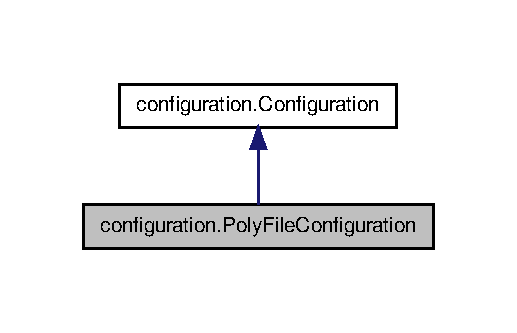
\includegraphics[width=248pt]{classconfiguration_1_1PolyFileConfiguration__inherit__graph}
\end{center}
\end{figure}


Collaboration diagram for configuration.\-Poly\-File\-Configuration\-:\nopagebreak
\begin{figure}[H]
\begin{center}
\leavevmode
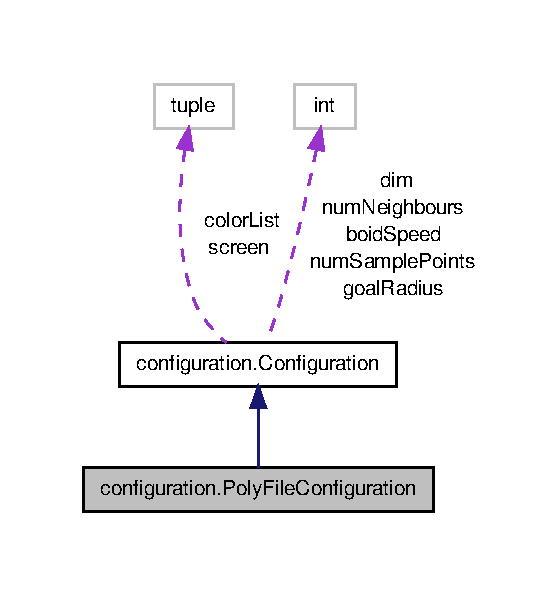
\includegraphics[width=269pt]{classconfiguration_1_1PolyFileConfiguration__coll__graph}
\end{center}
\end{figure}
\subsection*{Public Member Functions}
\begin{DoxyCompactItemize}
\item 
def \hyperlink{classconfiguration_1_1PolyFileConfiguration_ad68553a7fd263204c69800782fdd03a8}{init\-Vars}
\begin{DoxyCompactList}\small\item\em Parses the file to get the obstacle list. \end{DoxyCompactList}\end{DoxyCompactItemize}
\subsection*{Public Attributes}
\begin{DoxyCompactItemize}
\item 
\hyperlink{classconfiguration_1_1PolyFileConfiguration_a4ea5eea95680f3bfdad4adce0578a0f0}{obstacle\-List}
\begin{DoxyCompactList}\small\item\em List of obstacles. \end{DoxyCompactList}\item 
\hyperlink{classconfiguration_1_1PolyFileConfiguration_ae5c780baacd4b800d1646a29a8608cbf}{start\-Point}
\begin{DoxyCompactList}\small\item\em Starting point. \end{DoxyCompactList}\item 
\hyperlink{classconfiguration_1_1PolyFileConfiguration_acb9da93ddecef1bb34bbce601473f0f1}{end\-Point}
\begin{DoxyCompactList}\small\item\em Ending point. \end{DoxyCompactList}\item 
\hyperlink{classconfiguration_1_1PolyFileConfiguration_a075aa5177145a1041468f24e4829e8e8}{prm\-Gen}
\begin{DoxyCompactList}\small\item\em Object containing variables and mehtods for the global planner. \end{DoxyCompactList}\item 
\hyperlink{classconfiguration_1_1PolyFileConfiguration_a2fd4dfe65bb97105e3ff146d125849df}{goal\-List}
\begin{DoxyCompactList}\small\item\em List of intermediate goals derived by the global planner. \end{DoxyCompactList}\item 
\hyperlink{classconfiguration_1_1PolyFileConfiguration_a34104bbe3eb34147465a4d9e05d6c6b6}{boid\-List}
\begin{DoxyCompactList}\small\item\em List of boids in the flock. \end{DoxyCompactList}\end{DoxyCompactItemize}
\subsection*{Additional Inherited Members}


\subsection{Detailed Description}
Extends the \hyperlink{classconfiguration_1_1Configuration}{Configuration} class. 

This configuration gets the obstacles from .map files that have been created. 

Definition at line 44 of file configuration.\-py.



\subsection{Member Function Documentation}
\hypertarget{classconfiguration_1_1PolyFileConfiguration_ad68553a7fd263204c69800782fdd03a8}{\index{configuration\-::\-Poly\-File\-Configuration@{configuration\-::\-Poly\-File\-Configuration}!init\-Vars@{init\-Vars}}
\index{init\-Vars@{init\-Vars}!configuration::PolyFileConfiguration@{configuration\-::\-Poly\-File\-Configuration}}
\subsubsection[{init\-Vars}]{\setlength{\rightskip}{0pt plus 5cm}def configuration.\-Poly\-File\-Configuration.\-init\-Vars (
\begin{DoxyParamCaption}
\item[{}]{self, }
\item[{}]{start\-Point, }
\item[{}]{end\-Point, }
\item[{}]{flock\-Size, }
\item[{}]{filename = {\ttfamily \char`\"{}maps/m1.map\char`\"{}}}
\end{DoxyParamCaption}
)}}\label{classconfiguration_1_1PolyFileConfiguration_ad68553a7fd263204c69800782fdd03a8}


Parses the file to get the obstacle list. 

Creates a P\-R\-M generator to create a global map of the environment. Gets the list of intermediate goals. Also, creates the list of boids used in the simulation 
\begin{DoxyParams}{Parameters}
{\em start\-Point} & The starting point for the boids \\
\hline
{\em end\-Point} & The ending point for the boids \\
\hline
{\em flock\-Size} & The size of the flock (number of boids) \\
\hline
{\em filename} & The name of the file that contains the environment map \\
\hline
\end{DoxyParams}


Definition at line 55 of file configuration.\-py.



\subsection{Member Data Documentation}
\hypertarget{classconfiguration_1_1PolyFileConfiguration_a34104bbe3eb34147465a4d9e05d6c6b6}{\index{configuration\-::\-Poly\-File\-Configuration@{configuration\-::\-Poly\-File\-Configuration}!boid\-List@{boid\-List}}
\index{boid\-List@{boid\-List}!configuration::PolyFileConfiguration@{configuration\-::\-Poly\-File\-Configuration}}
\subsubsection[{boid\-List}]{\setlength{\rightskip}{0pt plus 5cm}configuration.\-Poly\-File\-Configuration.\-boid\-List}}\label{classconfiguration_1_1PolyFileConfiguration_a34104bbe3eb34147465a4d9e05d6c6b6}


List of boids in the flock. 



Definition at line 73 of file configuration.\-py.

\hypertarget{classconfiguration_1_1PolyFileConfiguration_acb9da93ddecef1bb34bbce601473f0f1}{\index{configuration\-::\-Poly\-File\-Configuration@{configuration\-::\-Poly\-File\-Configuration}!end\-Point@{end\-Point}}
\index{end\-Point@{end\-Point}!configuration::PolyFileConfiguration@{configuration\-::\-Poly\-File\-Configuration}}
\subsubsection[{end\-Point}]{\setlength{\rightskip}{0pt plus 5cm}configuration.\-Poly\-File\-Configuration.\-end\-Point}}\label{classconfiguration_1_1PolyFileConfiguration_acb9da93ddecef1bb34bbce601473f0f1}


Ending point. 



Definition at line 64 of file configuration.\-py.

\hypertarget{classconfiguration_1_1PolyFileConfiguration_a2fd4dfe65bb97105e3ff146d125849df}{\index{configuration\-::\-Poly\-File\-Configuration@{configuration\-::\-Poly\-File\-Configuration}!goal\-List@{goal\-List}}
\index{goal\-List@{goal\-List}!configuration::PolyFileConfiguration@{configuration\-::\-Poly\-File\-Configuration}}
\subsubsection[{goal\-List}]{\setlength{\rightskip}{0pt plus 5cm}configuration.\-Poly\-File\-Configuration.\-goal\-List}}\label{classconfiguration_1_1PolyFileConfiguration_a2fd4dfe65bb97105e3ff146d125849df}


List of intermediate goals derived by the global planner. 



Definition at line 70 of file configuration.\-py.

\hypertarget{classconfiguration_1_1PolyFileConfiguration_a4ea5eea95680f3bfdad4adce0578a0f0}{\index{configuration\-::\-Poly\-File\-Configuration@{configuration\-::\-Poly\-File\-Configuration}!obstacle\-List@{obstacle\-List}}
\index{obstacle\-List@{obstacle\-List}!configuration::PolyFileConfiguration@{configuration\-::\-Poly\-File\-Configuration}}
\subsubsection[{obstacle\-List}]{\setlength{\rightskip}{0pt plus 5cm}configuration.\-Poly\-File\-Configuration.\-obstacle\-List}}\label{classconfiguration_1_1PolyFileConfiguration_a4ea5eea95680f3bfdad4adce0578a0f0}


List of obstacles. 



Definition at line 58 of file configuration.\-py.

\hypertarget{classconfiguration_1_1PolyFileConfiguration_a075aa5177145a1041468f24e4829e8e8}{\index{configuration\-::\-Poly\-File\-Configuration@{configuration\-::\-Poly\-File\-Configuration}!prm\-Gen@{prm\-Gen}}
\index{prm\-Gen@{prm\-Gen}!configuration::PolyFileConfiguration@{configuration\-::\-Poly\-File\-Configuration}}
\subsubsection[{prm\-Gen}]{\setlength{\rightskip}{0pt plus 5cm}configuration.\-Poly\-File\-Configuration.\-prm\-Gen}}\label{classconfiguration_1_1PolyFileConfiguration_a075aa5177145a1041468f24e4829e8e8}


Object containing variables and mehtods for the global planner. 



Definition at line 67 of file configuration.\-py.

\hypertarget{classconfiguration_1_1PolyFileConfiguration_ae5c780baacd4b800d1646a29a8608cbf}{\index{configuration\-::\-Poly\-File\-Configuration@{configuration\-::\-Poly\-File\-Configuration}!start\-Point@{start\-Point}}
\index{start\-Point@{start\-Point}!configuration::PolyFileConfiguration@{configuration\-::\-Poly\-File\-Configuration}}
\subsubsection[{start\-Point}]{\setlength{\rightskip}{0pt plus 5cm}configuration.\-Poly\-File\-Configuration.\-start\-Point}}\label{classconfiguration_1_1PolyFileConfiguration_ae5c780baacd4b800d1646a29a8608cbf}


Starting point. 



Definition at line 61 of file configuration.\-py.



The documentation for this class was generated from the following file\-:\begin{DoxyCompactItemize}
\item 
code/\hyperlink{configuration_8py}{configuration.\-py (\-Concurrent Versions System (\-C\-V\-S) 1.\-12.\-13-\/\-Mir\-Debian-\/9 (client/server))}\end{DoxyCompactItemize}

\hypertarget{classobstacle_1_1PolyObstacle}{\section{obstacle.\-Poly\-Obstacle Class Reference}
\label{classobstacle_1_1PolyObstacle}\index{obstacle.\-Poly\-Obstacle@{obstacle.\-Poly\-Obstacle}}
}


Object that represents the an obstacle represented by a series of points (in the node list) which make up a set of lines.  


\subsection*{Public Member Functions}
\begin{DoxyCompactItemize}
\item 
def \hyperlink{classobstacle_1_1PolyObstacle_aa92e181aa910e2cd8c110047fe10dc83}{\-\_\-\-\_\-init\-\_\-\-\_\-}
\begin{DoxyCompactList}\small\item\em Creates a \hyperlink{classobstacle_1_1PolyObstacle}{Poly\-Obstacle} instance and initializes certain global variables. \end{DoxyCompactList}\item 
def \hyperlink{classobstacle_1_1PolyObstacle_a55c9604219c6622ad4a633c62fdbb058}{remove\-Self\-From\-Obstacle\-List}
\begin{DoxyCompactList}\small\item\em Removes self from obstacle list. \end{DoxyCompactList}\item 
def \hyperlink{classobstacle_1_1PolyObstacle_a3392ccb4d22e752b0f150af354b16862}{norm}
\begin{DoxyCompactList}\small\item\em Gets the Eulidean distance between p1 and p2. \end{DoxyCompactList}\item 
def \hyperlink{classobstacle_1_1PolyObstacle_ab2833da8e0c16a191ae373af40a75b46}{estimate\-Poly}
\begin{DoxyCompactList}\small\item\em Tries to estimate the polygon as a circle (very useful for environments with many obstacles i.\-e. \end{DoxyCompactList}\item 
def \hyperlink{classobstacle_1_1PolyObstacle_a2a3283cffb3239c8777b85a83af5ee8c}{detect\-Collision}
\begin{DoxyCompactList}\small\item\em Detects a if there is a collision with the obstacle and the line $<$p\-Start, p\-End$>$ \end{DoxyCompactList}\item 
def \hyperlink{classobstacle_1_1PolyObstacle_a43adce887280997dfb49067e741f54db}{get\-Closest\-Point}
\begin{DoxyCompactList}\small\item\em Gets the closest point on line $<$a, b$>$ to point p. \end{DoxyCompactList}\item 
def \hyperlink{classobstacle_1_1PolyObstacle_a646f5fc4ba3e67c98c2313f4493b6a08}{rayintersectseg}
\begin{DoxyCompactList}\small\item\em Determines if a ray from point p intersects with an edge, edge. \end{DoxyCompactList}\item 
def \hyperlink{classobstacle_1_1PolyObstacle_a4647d9efa8fb20d7b464ee5faa8fd7f4}{point\-In\-Poly}
\begin{DoxyCompactList}\small\item\em Determines if a point p is inside the polygon represented by this \hyperlink{classobstacle_1_1PolyObstacle}{Poly\-Obstacle} object. \end{DoxyCompactList}\item 
def \hyperlink{classobstacle_1_1PolyObstacle_af71f01fca50193a5e5372c2507661ada}{point\-Allowed}
\begin{DoxyCompactList}\small\item\em Checks if a point is allowed, meaning no collisions occur. \end{DoxyCompactList}\item 
def \hyperlink{classobstacle_1_1PolyObstacle_af866b6f101194b8a8731f2394fdc247e}{get\-Point}
\begin{DoxyCompactList}\small\item\em Gets the closest point from the polygon to p. \end{DoxyCompactList}\item 
def \hyperlink{classobstacle_1_1PolyObstacle_a205face22efbad01fd4c96fbe73321fd}{get\-Radius}
\begin{DoxyCompactList}\small\item\em Gets the 'radius' of the checking point. \end{DoxyCompactList}\item 
def \hyperlink{classobstacle_1_1PolyObstacle_af4f36a0612aa485298e12cd70a2677cb}{check\-Collision\-With\-Other\-Obstacles}
\begin{DoxyCompactList}\small\item\em Check to see if there is a collision with a static obstacle. \end{DoxyCompactList}\item 
def \hyperlink{classobstacle_1_1PolyObstacle_a8d4b0d3a614af138881a2f93d93f028a}{translate}
\begin{DoxyCompactList}\small\item\em Translate obstacle. \end{DoxyCompactList}\item 
def \hyperlink{classobstacle_1_1PolyObstacle_a64c90b17b8ca249e30e0b040930798de}{determine\-\_\-last\-\_\-direction}
\item 
def \hyperlink{classobstacle_1_1PolyObstacle_a9b6945bd67258643ad471c965889d707}{change\-\_\-direction}
\begin{DoxyCompactList}\small\item\em Change direction. \end{DoxyCompactList}\item 
def \hyperlink{classobstacle_1_1PolyObstacle_a9b5b53a6b8ee6233de2ee394871ebe6e}{draw}
\begin{DoxyCompactList}\small\item\em Draws the polygon on the Py\-Game screen. \end{DoxyCompactList}\end{DoxyCompactItemize}
\subsection*{Public Attributes}
\begin{DoxyCompactItemize}
\item 
\hyperlink{classobstacle_1_1PolyObstacle_a125762f0b4a3c9ef8d75c81bc5bc608e}{nodes}
\begin{DoxyCompactList}\small\item\em A list of nodes used to represent the vertices. \end{DoxyCompactList}\item 
\hyperlink{classobstacle_1_1PolyObstacle_a73ce2986866adb38653645c5b84ec0ce}{colors}
\begin{DoxyCompactList}\small\item\em A dictionary of colors defined in pygame. \end{DoxyCompactList}\item 
\hyperlink{classobstacle_1_1PolyObstacle_ad65d210c167b0638ef317ef24670501c}{screen}
\begin{DoxyCompactList}\small\item\em The Py\-Game screen that is used to draw the obstacle. \end{DoxyCompactList}\item 
\hyperlink{classobstacle_1_1PolyObstacle_a999b6ef28126661fc8d54e1d86c094e0}{boundary}
\begin{DoxyCompactList}\small\item\em Bondaries of the simualation. \end{DoxyCompactList}\item 
\hyperlink{classobstacle_1_1PolyObstacle_a9667fa3bc98877420e2af4bb6d617576}{dynamic}
\begin{DoxyCompactList}\small\item\em Defines wether the obstacle is dynamic or not. \end{DoxyCompactList}\item 
\hyperlink{classobstacle_1_1PolyObstacle_adb043e45a95522cec92cd6ad35ca6595}{velocity}
\begin{DoxyCompactList}\small\item\em Velocity of the obstacle. \end{DoxyCompactList}\item 
\hyperlink{classobstacle_1_1PolyObstacle_af943155354bdf61ff754752819ff4013}{displacement}
\begin{DoxyCompactList}\small\item\em The displacement of the obstacle. \end{DoxyCompactList}\item 
\hyperlink{classobstacle_1_1PolyObstacle_a01bca757590d23eeee5c864472a7fbe6}{max\-\_\-displacement}
\begin{DoxyCompactList}\small\item\em Max displacement allowed. \end{DoxyCompactList}\item 
\hyperlink{classobstacle_1_1PolyObstacle_a7df678f9d9362489ba24e0dd9ed70efc}{obstacles}
\begin{DoxyCompactList}\small\item\em List of static obstacles. \end{DoxyCompactList}\item 
\hyperlink{classobstacle_1_1PolyObstacle_ae426e9296754e1ba96abcee3b86b3591}{avg\-Point}
\begin{DoxyCompactList}\small\item\em The average point in the polygon. \end{DoxyCompactList}\item 
\hyperlink{classobstacle_1_1PolyObstacle_a14e97b3f09f9ff21f36efc7a58759e5c}{max\-Dist}
\begin{DoxyCompactList}\small\item\em The maximum distance from any vertex and the average point. \end{DoxyCompactList}\end{DoxyCompactItemize}


\subsection{Detailed Description}
Object that represents the an obstacle represented by a series of points (in the node list) which make up a set of lines. 

These lines represent the exterior of an obstacle 

Definition at line 18 of file obstacle.\-py.



\subsection{Constructor \& Destructor Documentation}
\hypertarget{classobstacle_1_1PolyObstacle_aa92e181aa910e2cd8c110047fe10dc83}{\index{obstacle\-::\-Poly\-Obstacle@{obstacle\-::\-Poly\-Obstacle}!\-\_\-\-\_\-init\-\_\-\-\_\-@{\-\_\-\-\_\-init\-\_\-\-\_\-}}
\index{\-\_\-\-\_\-init\-\_\-\-\_\-@{\-\_\-\-\_\-init\-\_\-\-\_\-}!obstacle::PolyObstacle@{obstacle\-::\-Poly\-Obstacle}}
\subsubsection[{\-\_\-\-\_\-init\-\_\-\-\_\-}]{\setlength{\rightskip}{0pt plus 5cm}def obstacle.\-Poly\-Obstacle.\-\_\-\-\_\-init\-\_\-\-\_\- (
\begin{DoxyParamCaption}
\item[{}]{self, }
\item[{}]{\-\_\-nodes, }
\item[{}]{\-\_\-screen, }
\item[{}]{kwargs}
\end{DoxyParamCaption}
)}}\label{classobstacle_1_1PolyObstacle_aa92e181aa910e2cd8c110047fe10dc83}


Creates a \hyperlink{classobstacle_1_1PolyObstacle}{Poly\-Obstacle} instance and initializes certain global variables. 


\begin{DoxyParams}{Parameters}
{\em \-\_\-nodes} & A list of nodes used to represent the vertices of the polygon \\
\hline
{\em \-\_\-screen} & The Py\-Game screen that is used to draw the obstacle \\
\hline
\end{DoxyParams}


Definition at line 27 of file obstacle.\-py.



\subsection{Member Function Documentation}
\hypertarget{classobstacle_1_1PolyObstacle_a9b6945bd67258643ad471c965889d707}{\index{obstacle\-::\-Poly\-Obstacle@{obstacle\-::\-Poly\-Obstacle}!change\-\_\-direction@{change\-\_\-direction}}
\index{change\-\_\-direction@{change\-\_\-direction}!obstacle::PolyObstacle@{obstacle\-::\-Poly\-Obstacle}}
\subsubsection[{change\-\_\-direction}]{\setlength{\rightskip}{0pt plus 5cm}def obstacle.\-Poly\-Obstacle.\-change\-\_\-direction (
\begin{DoxyParamCaption}
\item[{}]{self, }
\item[{}]{force\-\_\-change = {\ttfamily False}, }
\item[{}]{direction = {\ttfamily None}}
\end{DoxyParamCaption}
)}}\label{classobstacle_1_1PolyObstacle_a9b6945bd67258643ad471c965889d707}


Change direction. 



Definition at line 434 of file obstacle.\-py.



Here is the call graph for this function\-:




Here is the caller graph for this function\-:


\hypertarget{classobstacle_1_1PolyObstacle_af4f36a0612aa485298e12cd70a2677cb}{\index{obstacle\-::\-Poly\-Obstacle@{obstacle\-::\-Poly\-Obstacle}!check\-Collision\-With\-Other\-Obstacles@{check\-Collision\-With\-Other\-Obstacles}}
\index{check\-Collision\-With\-Other\-Obstacles@{check\-Collision\-With\-Other\-Obstacles}!obstacle::PolyObstacle@{obstacle\-::\-Poly\-Obstacle}}
\subsubsection[{check\-Collision\-With\-Other\-Obstacles}]{\setlength{\rightskip}{0pt plus 5cm}def obstacle.\-Poly\-Obstacle.\-check\-Collision\-With\-Other\-Obstacles (
\begin{DoxyParamCaption}
\item[{}]{self, }
\item[{}]{node}
\end{DoxyParamCaption}
)}}\label{classobstacle_1_1PolyObstacle_af4f36a0612aa485298e12cd70a2677cb}


Check to see if there is a collision with a static obstacle. 



Definition at line 359 of file obstacle.\-py.



Here is the call graph for this function\-:




Here is the caller graph for this function\-:


\hypertarget{classobstacle_1_1PolyObstacle_a2a3283cffb3239c8777b85a83af5ee8c}{\index{obstacle\-::\-Poly\-Obstacle@{obstacle\-::\-Poly\-Obstacle}!detect\-Collision@{detect\-Collision}}
\index{detect\-Collision@{detect\-Collision}!obstacle::PolyObstacle@{obstacle\-::\-Poly\-Obstacle}}
\subsubsection[{detect\-Collision}]{\setlength{\rightskip}{0pt plus 5cm}def obstacle.\-Poly\-Obstacle.\-detect\-Collision (
\begin{DoxyParamCaption}
\item[{}]{self, }
\item[{}]{p\-Start, }
\item[{}]{p\-End}
\end{DoxyParamCaption}
)}}\label{classobstacle_1_1PolyObstacle_a2a3283cffb3239c8777b85a83af5ee8c}


Detects a if there is a collision with the obstacle and the line $<$p\-Start, p\-End$>$ 


\begin{DoxyParams}{Parameters}
{\em p\-Start} & The starting point of the line \\
\hline
{\em p\-End} & The ending point of the line \\
\hline
\end{DoxyParams}
\begin{DoxyReturn}{Returns}
A boolean value representing if a collision occurred 
\end{DoxyReturn}


Definition at line 114 of file obstacle.\-py.

\hypertarget{classobstacle_1_1PolyObstacle_a64c90b17b8ca249e30e0b040930798de}{\index{obstacle\-::\-Poly\-Obstacle@{obstacle\-::\-Poly\-Obstacle}!determine\-\_\-last\-\_\-direction@{determine\-\_\-last\-\_\-direction}}
\index{determine\-\_\-last\-\_\-direction@{determine\-\_\-last\-\_\-direction}!obstacle::PolyObstacle@{obstacle\-::\-Poly\-Obstacle}}
\subsubsection[{determine\-\_\-last\-\_\-direction}]{\setlength{\rightskip}{0pt plus 5cm}def obstacle.\-Poly\-Obstacle.\-determine\-\_\-last\-\_\-direction (
\begin{DoxyParamCaption}
\item[{}]{self}
\end{DoxyParamCaption}
)}}\label{classobstacle_1_1PolyObstacle_a64c90b17b8ca249e30e0b040930798de}


Definition at line 418 of file obstacle.\-py.



Here is the caller graph for this function\-:


\hypertarget{classobstacle_1_1PolyObstacle_a9b5b53a6b8ee6233de2ee394871ebe6e}{\index{obstacle\-::\-Poly\-Obstacle@{obstacle\-::\-Poly\-Obstacle}!draw@{draw}}
\index{draw@{draw}!obstacle::PolyObstacle@{obstacle\-::\-Poly\-Obstacle}}
\subsubsection[{draw}]{\setlength{\rightskip}{0pt plus 5cm}def obstacle.\-Poly\-Obstacle.\-draw (
\begin{DoxyParamCaption}
\item[{}]{self}
\end{DoxyParamCaption}
)}}\label{classobstacle_1_1PolyObstacle_a9b5b53a6b8ee6233de2ee394871ebe6e}


Draws the polygon on the Py\-Game screen. 



Definition at line 478 of file obstacle.\-py.



Here is the call graph for this function\-:


\hypertarget{classobstacle_1_1PolyObstacle_ab2833da8e0c16a191ae373af40a75b46}{\index{obstacle\-::\-Poly\-Obstacle@{obstacle\-::\-Poly\-Obstacle}!estimate\-Poly@{estimate\-Poly}}
\index{estimate\-Poly@{estimate\-Poly}!obstacle::PolyObstacle@{obstacle\-::\-Poly\-Obstacle}}
\subsubsection[{estimate\-Poly}]{\setlength{\rightskip}{0pt plus 5cm}def obstacle.\-Poly\-Obstacle.\-estimate\-Poly (
\begin{DoxyParamCaption}
\item[{}]{self}
\end{DoxyParamCaption}
)}}\label{classobstacle_1_1PolyObstacle_ab2833da8e0c16a191ae373af40a75b46}


Tries to estimate the polygon as a circle (very useful for environments with many obstacles i.\-e. 

a random field of obstacles) 

Definition at line 81 of file obstacle.\-py.

\hypertarget{classobstacle_1_1PolyObstacle_a43adce887280997dfb49067e741f54db}{\index{obstacle\-::\-Poly\-Obstacle@{obstacle\-::\-Poly\-Obstacle}!get\-Closest\-Point@{get\-Closest\-Point}}
\index{get\-Closest\-Point@{get\-Closest\-Point}!obstacle::PolyObstacle@{obstacle\-::\-Poly\-Obstacle}}
\subsubsection[{get\-Closest\-Point}]{\setlength{\rightskip}{0pt plus 5cm}def obstacle.\-Poly\-Obstacle.\-get\-Closest\-Point (
\begin{DoxyParamCaption}
\item[{}]{self, }
\item[{}]{a, }
\item[{}]{b, }
\item[{}]{p}
\end{DoxyParamCaption}
)}}\label{classobstacle_1_1PolyObstacle_a43adce887280997dfb49067e741f54db}


Gets the closest point on line $<$a, b$>$ to point p. 


\begin{DoxyParams}{Parameters}
{\em a} & The starting point on the line \\
\hline
{\em b} & The ending point of the line \\
\hline
{\em p} & The point in which the closest distance will be checked \\
\hline
\end{DoxyParams}
\begin{DoxyReturn}{Returns}
The closest point on line $<$a, b$>$ to point p 
\end{DoxyReturn}


Definition at line 171 of file obstacle.\-py.



Here is the call graph for this function\-:\nopagebreak
\begin{figure}[H]
\begin{center}
\leavevmode
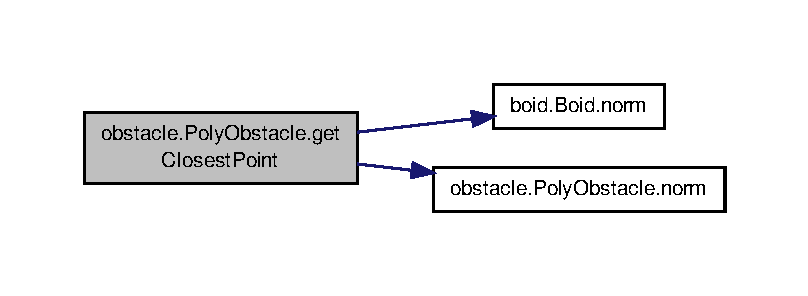
\includegraphics[width=350pt]{classobstacle_1_1PolyObstacle_a43adce887280997dfb49067e741f54db_cgraph}
\end{center}
\end{figure}




Here is the caller graph for this function\-:\nopagebreak
\begin{figure}[H]
\begin{center}
\leavevmode
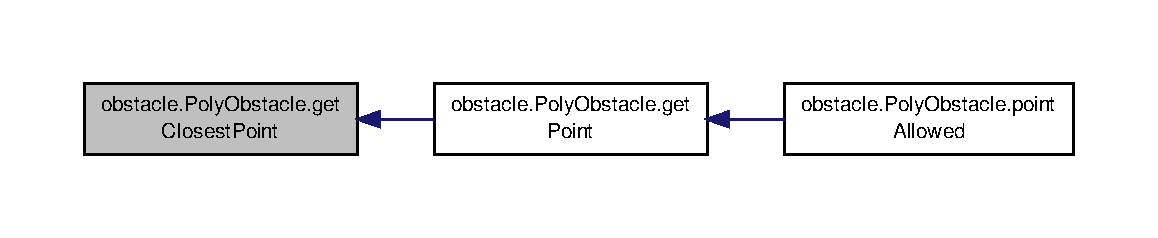
\includegraphics[width=350pt]{classobstacle_1_1PolyObstacle_a43adce887280997dfb49067e741f54db_icgraph}
\end{center}
\end{figure}


\hypertarget{classobstacle_1_1PolyObstacle_af866b6f101194b8a8731f2394fdc247e}{\index{obstacle\-::\-Poly\-Obstacle@{obstacle\-::\-Poly\-Obstacle}!get\-Point@{get\-Point}}
\index{get\-Point@{get\-Point}!obstacle::PolyObstacle@{obstacle\-::\-Poly\-Obstacle}}
\subsubsection[{get\-Point}]{\setlength{\rightskip}{0pt plus 5cm}def obstacle.\-Poly\-Obstacle.\-get\-Point (
\begin{DoxyParamCaption}
\item[{}]{self, }
\item[{}]{p}
\end{DoxyParamCaption}
)}}\label{classobstacle_1_1PolyObstacle_af866b6f101194b8a8731f2394fdc247e}


Gets the closest point from the polygon to p. 


\begin{DoxyParams}{Parameters}
{\em p} & The point to be checked \\
\hline
\end{DoxyParams}
\begin{DoxyReturn}{Returns}
The closest point that lies on the polygon exterior to p 
\end{DoxyReturn}


Definition at line 323 of file obstacle.\-py.



Here is the call graph for this function\-:\nopagebreak
\begin{figure}[H]
\begin{center}
\leavevmode
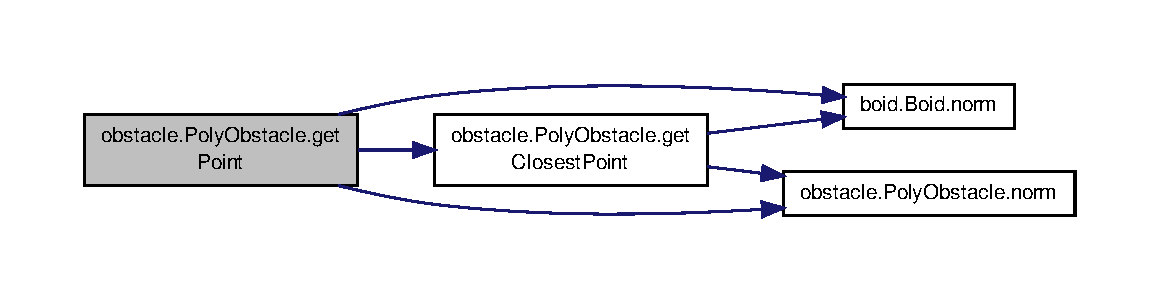
\includegraphics[width=350pt]{classobstacle_1_1PolyObstacle_af866b6f101194b8a8731f2394fdc247e_cgraph}
\end{center}
\end{figure}




Here is the caller graph for this function\-:\nopagebreak
\begin{figure}[H]
\begin{center}
\leavevmode
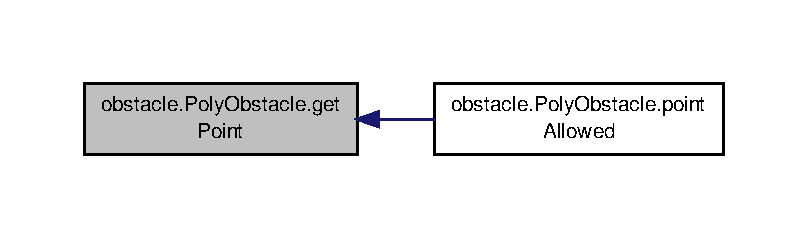
\includegraphics[width=350pt]{classobstacle_1_1PolyObstacle_af866b6f101194b8a8731f2394fdc247e_icgraph}
\end{center}
\end{figure}


\hypertarget{classobstacle_1_1PolyObstacle_a205face22efbad01fd4c96fbe73321fd}{\index{obstacle\-::\-Poly\-Obstacle@{obstacle\-::\-Poly\-Obstacle}!get\-Radius@{get\-Radius}}
\index{get\-Radius@{get\-Radius}!obstacle::PolyObstacle@{obstacle\-::\-Poly\-Obstacle}}
\subsubsection[{get\-Radius}]{\setlength{\rightskip}{0pt plus 5cm}def obstacle.\-Poly\-Obstacle.\-get\-Radius (
\begin{DoxyParamCaption}
\item[{}]{self}
\end{DoxyParamCaption}
)}}\label{classobstacle_1_1PolyObstacle_a205face22efbad01fd4c96fbe73321fd}


Gets the 'radius' of the checking point. 

Only used for conformity with circle obstacles that have not been included in this repository \begin{DoxyReturn}{Returns}
1 
\end{DoxyReturn}


Definition at line 352 of file obstacle.\-py.

\hypertarget{classobstacle_1_1PolyObstacle_a3392ccb4d22e752b0f150af354b16862}{\index{obstacle\-::\-Poly\-Obstacle@{obstacle\-::\-Poly\-Obstacle}!norm@{norm}}
\index{norm@{norm}!obstacle::PolyObstacle@{obstacle\-::\-Poly\-Obstacle}}
\subsubsection[{norm}]{\setlength{\rightskip}{0pt plus 5cm}def obstacle.\-Poly\-Obstacle.\-norm (
\begin{DoxyParamCaption}
\item[{}]{self, }
\item[{}]{p1, }
\item[{}]{p2}
\end{DoxyParamCaption}
)}}\label{classobstacle_1_1PolyObstacle_a3392ccb4d22e752b0f150af354b16862}


Gets the Eulidean distance between p1 and p2. 


\begin{DoxyParams}{Parameters}
{\em p1,p2} & Points in space \\
\hline
\end{DoxyParams}
\begin{DoxyReturn}{Returns}
The distance between p1 and p2 
\end{DoxyReturn}


Definition at line 73 of file obstacle.\-py.



Here is the caller graph for this function\-:
\nopagebreak
\begin{figure}[H]
\begin{center}
\leavevmode
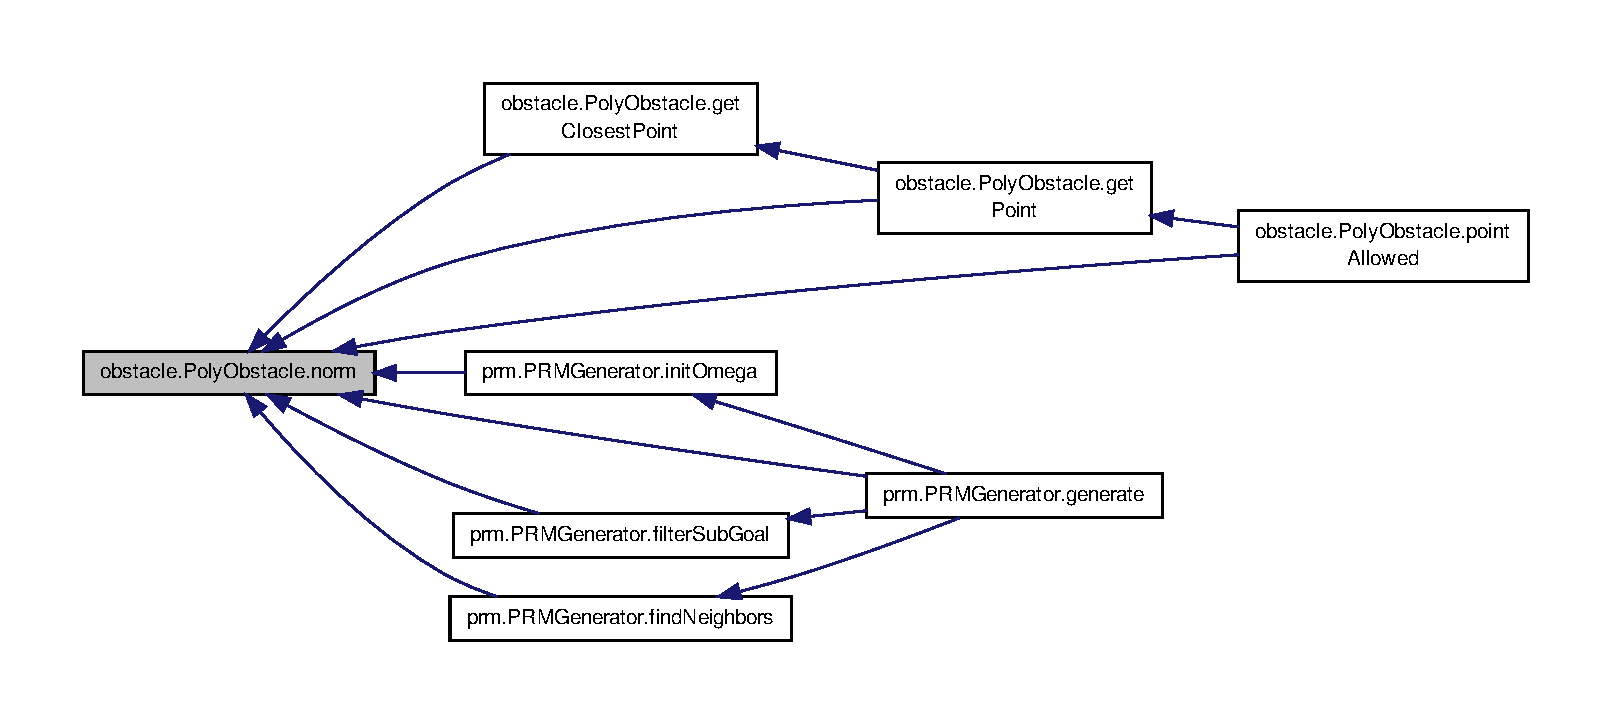
\includegraphics[width=350pt]{classobstacle_1_1PolyObstacle_a3392ccb4d22e752b0f150af354b16862_icgraph}
\end{center}
\end{figure}


\hypertarget{classobstacle_1_1PolyObstacle_af71f01fca50193a5e5372c2507661ada}{\index{obstacle\-::\-Poly\-Obstacle@{obstacle\-::\-Poly\-Obstacle}!point\-Allowed@{point\-Allowed}}
\index{point\-Allowed@{point\-Allowed}!obstacle::PolyObstacle@{obstacle\-::\-Poly\-Obstacle}}
\subsubsection[{point\-Allowed}]{\setlength{\rightskip}{0pt plus 5cm}def obstacle.\-Poly\-Obstacle.\-point\-Allowed (
\begin{DoxyParamCaption}
\item[{}]{self, }
\item[{}]{b, }
\item[{}]{p}
\end{DoxyParamCaption}
)}}\label{classobstacle_1_1PolyObstacle_af71f01fca50193a5e5372c2507661ada}


Checks if a point is allowed, meaning no collisions occur. 


\begin{DoxyParams}{Parameters}
{\em b} & The boid object that will be checked \\
\hline
{\em p} & The point that will be checked \\
\hline
\end{DoxyParams}
\begin{DoxyReturn}{Returns}
True if allowed, false otherwise 
\end{DoxyReturn}


Definition at line 303 of file obstacle.\-py.



Here is the call graph for this function\-:\nopagebreak
\begin{figure}[H]
\begin{center}
\leavevmode
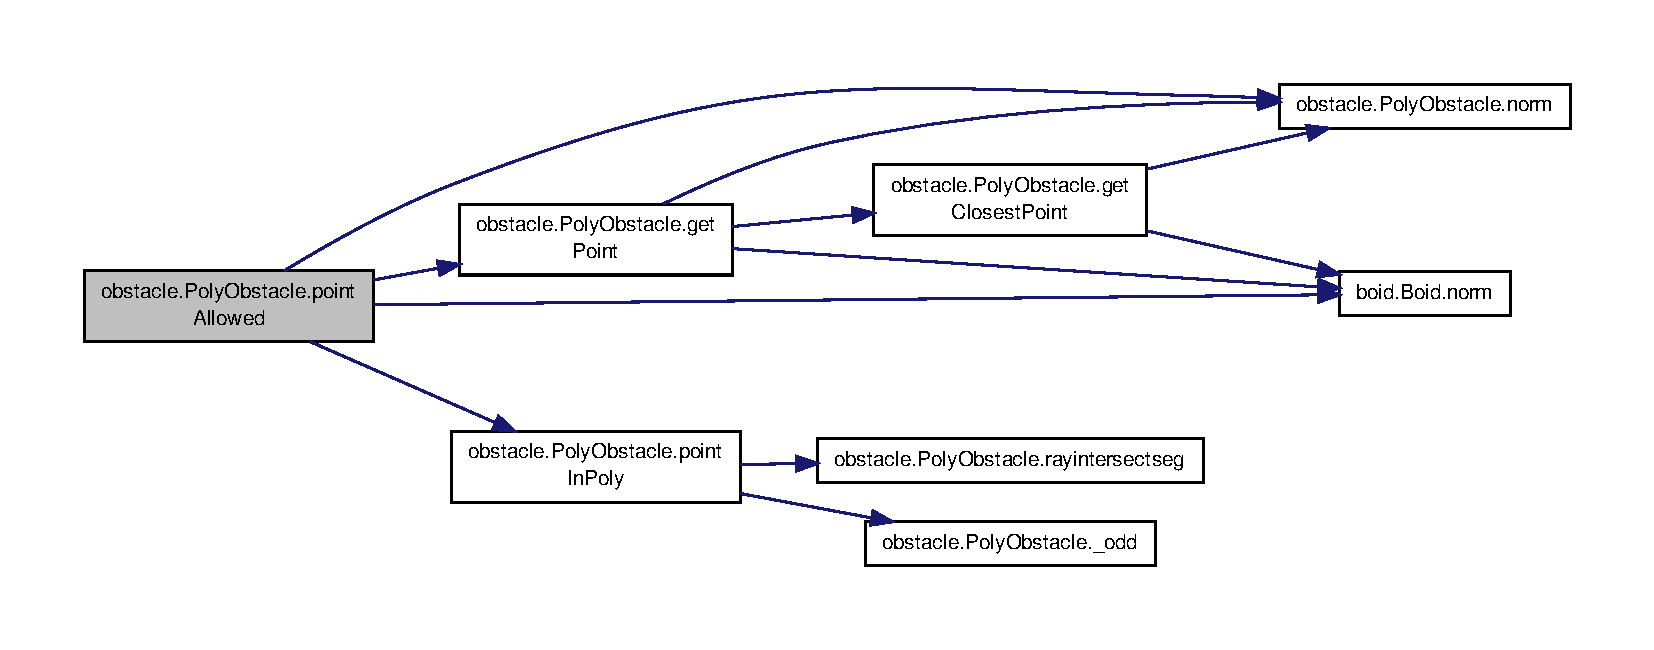
\includegraphics[width=350pt]{classobstacle_1_1PolyObstacle_af71f01fca50193a5e5372c2507661ada_cgraph}
\end{center}
\end{figure}


\hypertarget{classobstacle_1_1PolyObstacle_a4647d9efa8fb20d7b464ee5faa8fd7f4}{\index{obstacle\-::\-Poly\-Obstacle@{obstacle\-::\-Poly\-Obstacle}!point\-In\-Poly@{point\-In\-Poly}}
\index{point\-In\-Poly@{point\-In\-Poly}!obstacle::PolyObstacle@{obstacle\-::\-Poly\-Obstacle}}
\subsubsection[{point\-In\-Poly}]{\setlength{\rightskip}{0pt plus 5cm}def obstacle.\-Poly\-Obstacle.\-point\-In\-Poly (
\begin{DoxyParamCaption}
\item[{}]{self, }
\item[{}]{p}
\end{DoxyParamCaption}
)}}\label{classobstacle_1_1PolyObstacle_a4647d9efa8fb20d7b464ee5faa8fd7f4}


Determines if a point p is inside the polygon represented by this \hyperlink{classobstacle_1_1PolyObstacle}{Poly\-Obstacle} object. 

It does this by checking the number ray intersections that occur is odd or even. If the number is odd, the point is inside the polygon, otherwise it is not. 
\begin{DoxyParams}{Parameters}
{\em p} & The point to be checked \\
\hline
\end{DoxyParams}
\begin{DoxyReturn}{Returns}
True if the point is in the polygon and false otherwise 
\end{DoxyReturn}


Definition at line 286 of file obstacle.\-py.



Here is the call graph for this function\-:\nopagebreak
\begin{figure}[H]
\begin{center}
\leavevmode
\includegraphics[width=350pt]{classobstacle_1_1PolyObstacle_a4647d9efa8fb20d7b464ee5faa8fd7f4_cgraph}
\end{center}
\end{figure}




Here is the caller graph for this function\-:\nopagebreak
\begin{figure}[H]
\begin{center}
\leavevmode
\includegraphics[width=350pt]{classobstacle_1_1PolyObstacle_a4647d9efa8fb20d7b464ee5faa8fd7f4_icgraph}
\end{center}
\end{figure}


\hypertarget{classobstacle_1_1PolyObstacle_a646f5fc4ba3e67c98c2313f4493b6a08}{\index{obstacle\-::\-Poly\-Obstacle@{obstacle\-::\-Poly\-Obstacle}!rayintersectseg@{rayintersectseg}}
\index{rayintersectseg@{rayintersectseg}!obstacle::PolyObstacle@{obstacle\-::\-Poly\-Obstacle}}
\subsubsection[{rayintersectseg}]{\setlength{\rightskip}{0pt plus 5cm}def obstacle.\-Poly\-Obstacle.\-rayintersectseg (
\begin{DoxyParamCaption}
\item[{}]{self, }
\item[{}]{p, }
\item[{}]{edge}
\end{DoxyParamCaption}
)}}\label{classobstacle_1_1PolyObstacle_a646f5fc4ba3e67c98c2313f4493b6a08}


Determines if a ray from point p intersects with an edge, edge. 

\begin{DoxyVerb}     Used to determine if a point p in inside the polygon
\end{DoxyVerb}
 
\begin{DoxyParams}{Parameters}
{\em p} & The point to be checked \\
\hline
{\em edge} & The edge that will be checked \\
\hline
\end{DoxyParams}
\begin{DoxyReturn}{Returns}
True if a ray from point p intersects with edge and false otherwise 
\end{DoxyReturn}


Definition at line 239 of file obstacle.\-py.



Here is the caller graph for this function\-:\nopagebreak
\begin{figure}[H]
\begin{center}
\leavevmode
\includegraphics[width=350pt]{classobstacle_1_1PolyObstacle_a646f5fc4ba3e67c98c2313f4493b6a08_icgraph}
\end{center}
\end{figure}


\hypertarget{classobstacle_1_1PolyObstacle_a55c9604219c6622ad4a633c62fdbb058}{\index{obstacle\-::\-Poly\-Obstacle@{obstacle\-::\-Poly\-Obstacle}!remove\-Self\-From\-Obstacle\-List@{remove\-Self\-From\-Obstacle\-List}}
\index{remove\-Self\-From\-Obstacle\-List@{remove\-Self\-From\-Obstacle\-List}!obstacle::PolyObstacle@{obstacle\-::\-Poly\-Obstacle}}
\subsubsection[{remove\-Self\-From\-Obstacle\-List}]{\setlength{\rightskip}{0pt plus 5cm}def obstacle.\-Poly\-Obstacle.\-remove\-Self\-From\-Obstacle\-List (
\begin{DoxyParamCaption}
\item[{}]{self}
\end{DoxyParamCaption}
)}}\label{classobstacle_1_1PolyObstacle_a55c9604219c6622ad4a633c62fdbb058}


Removes self from obstacle list. 



Definition at line 62 of file obstacle.\-py.

\hypertarget{classobstacle_1_1PolyObstacle_a8d4b0d3a614af138881a2f93d93f028a}{\index{obstacle\-::\-Poly\-Obstacle@{obstacle\-::\-Poly\-Obstacle}!translate@{translate}}
\index{translate@{translate}!obstacle::PolyObstacle@{obstacle\-::\-Poly\-Obstacle}}
\subsubsection[{translate}]{\setlength{\rightskip}{0pt plus 5cm}def obstacle.\-Poly\-Obstacle.\-translate (
\begin{DoxyParamCaption}
\item[{}]{self}
\end{DoxyParamCaption}
)}}\label{classobstacle_1_1PolyObstacle_a8d4b0d3a614af138881a2f93d93f028a}


Translate obstacle. 



Definition at line 372 of file obstacle.\-py.



Here is the call graph for this function\-:




Here is the caller graph for this function\-:




\subsection{Member Data Documentation}
\hypertarget{classobstacle_1_1PolyObstacle_ae426e9296754e1ba96abcee3b86b3591}{\index{obstacle\-::\-Poly\-Obstacle@{obstacle\-::\-Poly\-Obstacle}!avg\-Point@{avg\-Point}}
\index{avg\-Point@{avg\-Point}!obstacle::PolyObstacle@{obstacle\-::\-Poly\-Obstacle}}
\subsubsection[{avg\-Point}]{\setlength{\rightskip}{0pt plus 5cm}obstacle.\-Poly\-Obstacle.\-avg\-Point}}\label{classobstacle_1_1PolyObstacle_ae426e9296754e1ba96abcee3b86b3591}


The average point in the polygon. 

Represents the center of the enclosing circle 

Definition at line 85 of file obstacle.\-py.

\hypertarget{classobstacle_1_1PolyObstacle_a999b6ef28126661fc8d54e1d86c094e0}{\index{obstacle\-::\-Poly\-Obstacle@{obstacle\-::\-Poly\-Obstacle}!boundary@{boundary}}
\index{boundary@{boundary}!obstacle::PolyObstacle@{obstacle\-::\-Poly\-Obstacle}}
\subsubsection[{boundary}]{\setlength{\rightskip}{0pt plus 5cm}obstacle.\-Poly\-Obstacle.\-boundary}}\label{classobstacle_1_1PolyObstacle_a999b6ef28126661fc8d54e1d86c094e0}


Bondaries of the simualation. 



Definition at line 39 of file obstacle.\-py.

\hypertarget{classobstacle_1_1PolyObstacle_a73ce2986866adb38653645c5b84ec0ce}{\index{obstacle\-::\-Poly\-Obstacle@{obstacle\-::\-Poly\-Obstacle}!colors@{colors}}
\index{colors@{colors}!obstacle::PolyObstacle@{obstacle\-::\-Poly\-Obstacle}}
\subsubsection[{colors}]{\setlength{\rightskip}{0pt plus 5cm}obstacle.\-Poly\-Obstacle.\-colors}}\label{classobstacle_1_1PolyObstacle_a73ce2986866adb38653645c5b84ec0ce}


A dictionary of colors defined in pygame. 



Definition at line 33 of file obstacle.\-py.

\hypertarget{classobstacle_1_1PolyObstacle_af943155354bdf61ff754752819ff4013}{\index{obstacle\-::\-Poly\-Obstacle@{obstacle\-::\-Poly\-Obstacle}!displacement@{displacement}}
\index{displacement@{displacement}!obstacle::PolyObstacle@{obstacle\-::\-Poly\-Obstacle}}
\subsubsection[{displacement}]{\setlength{\rightskip}{0pt plus 5cm}obstacle.\-Poly\-Obstacle.\-displacement}}\label{classobstacle_1_1PolyObstacle_af943155354bdf61ff754752819ff4013}


The displacement of the obstacle. 



Definition at line 48 of file obstacle.\-py.

\hypertarget{classobstacle_1_1PolyObstacle_a9667fa3bc98877420e2af4bb6d617576}{\index{obstacle\-::\-Poly\-Obstacle@{obstacle\-::\-Poly\-Obstacle}!dynamic@{dynamic}}
\index{dynamic@{dynamic}!obstacle::PolyObstacle@{obstacle\-::\-Poly\-Obstacle}}
\subsubsection[{dynamic}]{\setlength{\rightskip}{0pt plus 5cm}obstacle.\-Poly\-Obstacle.\-dynamic}}\label{classobstacle_1_1PolyObstacle_a9667fa3bc98877420e2af4bb6d617576}


Defines wether the obstacle is dynamic or not. 



Definition at line 42 of file obstacle.\-py.

\hypertarget{classobstacle_1_1PolyObstacle_a01bca757590d23eeee5c864472a7fbe6}{\index{obstacle\-::\-Poly\-Obstacle@{obstacle\-::\-Poly\-Obstacle}!max\-\_\-displacement@{max\-\_\-displacement}}
\index{max\-\_\-displacement@{max\-\_\-displacement}!obstacle::PolyObstacle@{obstacle\-::\-Poly\-Obstacle}}
\subsubsection[{max\-\_\-displacement}]{\setlength{\rightskip}{0pt plus 5cm}obstacle.\-Poly\-Obstacle.\-max\-\_\-displacement}}\label{classobstacle_1_1PolyObstacle_a01bca757590d23eeee5c864472a7fbe6}


Max displacement allowed. 



Definition at line 51 of file obstacle.\-py.

\hypertarget{classobstacle_1_1PolyObstacle_a14e97b3f09f9ff21f36efc7a58759e5c}{\index{obstacle\-::\-Poly\-Obstacle@{obstacle\-::\-Poly\-Obstacle}!max\-Dist@{max\-Dist}}
\index{max\-Dist@{max\-Dist}!obstacle::PolyObstacle@{obstacle\-::\-Poly\-Obstacle}}
\subsubsection[{max\-Dist}]{\setlength{\rightskip}{0pt plus 5cm}obstacle.\-Poly\-Obstacle.\-max\-Dist}}\label{classobstacle_1_1PolyObstacle_a14e97b3f09f9ff21f36efc7a58759e5c}


The maximum distance from any vertex and the average point. 



Definition at line 97 of file obstacle.\-py.

\hypertarget{classobstacle_1_1PolyObstacle_a125762f0b4a3c9ef8d75c81bc5bc608e}{\index{obstacle\-::\-Poly\-Obstacle@{obstacle\-::\-Poly\-Obstacle}!nodes@{nodes}}
\index{nodes@{nodes}!obstacle::PolyObstacle@{obstacle\-::\-Poly\-Obstacle}}
\subsubsection[{nodes}]{\setlength{\rightskip}{0pt plus 5cm}obstacle.\-Poly\-Obstacle.\-nodes}}\label{classobstacle_1_1PolyObstacle_a125762f0b4a3c9ef8d75c81bc5bc608e}


A list of nodes used to represent the vertices. 



Definition at line 30 of file obstacle.\-py.

\hypertarget{classobstacle_1_1PolyObstacle_a7df678f9d9362489ba24e0dd9ed70efc}{\index{obstacle\-::\-Poly\-Obstacle@{obstacle\-::\-Poly\-Obstacle}!obstacles@{obstacles}}
\index{obstacles@{obstacles}!obstacle::PolyObstacle@{obstacle\-::\-Poly\-Obstacle}}
\subsubsection[{obstacles}]{\setlength{\rightskip}{0pt plus 5cm}obstacle.\-Poly\-Obstacle.\-obstacles}}\label{classobstacle_1_1PolyObstacle_a7df678f9d9362489ba24e0dd9ed70efc}


List of static obstacles. 



Definition at line 54 of file obstacle.\-py.

\hypertarget{classobstacle_1_1PolyObstacle_ad65d210c167b0638ef317ef24670501c}{\index{obstacle\-::\-Poly\-Obstacle@{obstacle\-::\-Poly\-Obstacle}!screen@{screen}}
\index{screen@{screen}!obstacle::PolyObstacle@{obstacle\-::\-Poly\-Obstacle}}
\subsubsection[{screen}]{\setlength{\rightskip}{0pt plus 5cm}obstacle.\-Poly\-Obstacle.\-screen}}\label{classobstacle_1_1PolyObstacle_ad65d210c167b0638ef317ef24670501c}


The Py\-Game screen that is used to draw the obstacle. 



Definition at line 36 of file obstacle.\-py.

\hypertarget{classobstacle_1_1PolyObstacle_adb043e45a95522cec92cd6ad35ca6595}{\index{obstacle\-::\-Poly\-Obstacle@{obstacle\-::\-Poly\-Obstacle}!velocity@{velocity}}
\index{velocity@{velocity}!obstacle::PolyObstacle@{obstacle\-::\-Poly\-Obstacle}}
\subsubsection[{velocity}]{\setlength{\rightskip}{0pt plus 5cm}obstacle.\-Poly\-Obstacle.\-velocity}}\label{classobstacle_1_1PolyObstacle_adb043e45a95522cec92cd6ad35ca6595}


Velocity of the obstacle. 



Definition at line 45 of file obstacle.\-py.



The documentation for this class was generated from the following file\-:\begin{DoxyCompactItemize}
\item 
code/\hyperlink{obstacle_8py}{obstacle.\-py}\end{DoxyCompactItemize}

\hypertarget{classpriodict_1_1priorityDictionary}{\section{priodict.\-priority\-Dictionary Class Reference}
\label{classpriodict_1_1priorityDictionary}\index{priodict.\-priority\-Dictionary@{priodict.\-priority\-Dictionary}}
}


Inheritance diagram for priodict.\-priority\-Dictionary\-:\nopagebreak
\begin{figure}[H]
\begin{center}
\leavevmode
\includegraphics[width=204pt]{classpriodict_1_1priorityDictionary__inherit__graph}
\end{center}
\end{figure}


Collaboration diagram for priodict.\-priority\-Dictionary\-:\nopagebreak
\begin{figure}[H]
\begin{center}
\leavevmode
\includegraphics[width=204pt]{classpriodict_1_1priorityDictionary__coll__graph}
\end{center}
\end{figure}
\subsection*{Public Member Functions}
\begin{DoxyCompactItemize}
\item 
def \hyperlink{classpriodict_1_1priorityDictionary_a0b614c3f902b4ca714c9a8173c4ec3e3}{\-\_\-\-\_\-init\-\_\-\-\_\-}
\begin{DoxyCompactList}\small\item\em Initialize \hyperlink{classpriodict_1_1priorityDictionary}{priority\-Dictionary} by creating binary heap of pairs (value,key). \end{DoxyCompactList}\item 
def \hyperlink{classpriodict_1_1priorityDictionary_addbfef62eca26714c932482d2df9f14a}{smallest}
\begin{DoxyCompactList}\small\item\em Find smallest item after removing deleted items from heap. \end{DoxyCompactList}\item 
def \hyperlink{classpriodict_1_1priorityDictionary_ae2386d1d220c9be0c3193adf425423dd}{\-\_\-\-\_\-iter\-\_\-\-\_\-}
\begin{DoxyCompactList}\small\item\em Create destructive sorted iterator of \hyperlink{classpriodict_1_1priorityDictionary}{priority\-Dictionary}. \end{DoxyCompactList}\item 
def \hyperlink{classpriodict_1_1priorityDictionary_a862dc448352bd602da86d957a4752167}{\-\_\-\-\_\-setitem\-\_\-\-\_\-}
\begin{DoxyCompactList}\small\item\em Change value stored in dictionary and add corresponding pair to heap. \end{DoxyCompactList}\item 
def \hyperlink{classpriodict_1_1priorityDictionary_aaba46b716d256d1d0b79ec44a2195c19}{setdefault}
\begin{DoxyCompactList}\small\item\em Reimplement setdefault to call our customized {\bfseries setitem}. \end{DoxyCompactList}\end{DoxyCompactItemize}


\subsection{Detailed Description}


Definition at line 6 of file priodict.\-py.



\subsection{Constructor \& Destructor Documentation}
\hypertarget{classpriodict_1_1priorityDictionary_a0b614c3f902b4ca714c9a8173c4ec3e3}{\index{priodict\-::priority\-Dictionary@{priodict\-::priority\-Dictionary}!\-\_\-\-\_\-init\-\_\-\-\_\-@{\-\_\-\-\_\-init\-\_\-\-\_\-}}
\index{\-\_\-\-\_\-init\-\_\-\-\_\-@{\-\_\-\-\_\-init\-\_\-\-\_\-}!priodict::priorityDictionary@{priodict\-::priority\-Dictionary}}
\subsubsection[{\-\_\-\-\_\-init\-\_\-\-\_\-}]{\setlength{\rightskip}{0pt plus 5cm}def priodict.\-priority\-Dictionary.\-\_\-\-\_\-init\-\_\-\-\_\- (
\begin{DoxyParamCaption}
\item[{}]{self}
\end{DoxyParamCaption}
)}}\label{classpriodict_1_1priorityDictionary_a0b614c3f902b4ca714c9a8173c4ec3e3}


Initialize \hyperlink{classpriodict_1_1priorityDictionary}{priority\-Dictionary} by creating binary heap of pairs (value,key). 

Note that changing or removing a dict entry will not remove the old pair from the heap until it is found by \hyperlink{classpriodict_1_1priorityDictionary_addbfef62eca26714c932482d2df9f14a}{smallest()} or until the heap is rebuilt. 

Definition at line 12 of file priodict.\-py.



\subsection{Member Function Documentation}
\hypertarget{classpriodict_1_1priorityDictionary_ae2386d1d220c9be0c3193adf425423dd}{\index{priodict\-::priority\-Dictionary@{priodict\-::priority\-Dictionary}!\-\_\-\-\_\-iter\-\_\-\-\_\-@{\-\_\-\-\_\-iter\-\_\-\-\_\-}}
\index{\-\_\-\-\_\-iter\-\_\-\-\_\-@{\-\_\-\-\_\-iter\-\_\-\-\_\-}!priodict::priorityDictionary@{priodict\-::priority\-Dictionary}}
\subsubsection[{\-\_\-\-\_\-iter\-\_\-\-\_\-}]{\setlength{\rightskip}{0pt plus 5cm}def priodict.\-priority\-Dictionary.\-\_\-\-\_\-iter\-\_\-\-\_\- (
\begin{DoxyParamCaption}
\item[{}]{self}
\end{DoxyParamCaption}
)}}\label{classpriodict_1_1priorityDictionary_ae2386d1d220c9be0c3193adf425423dd}


Create destructive sorted iterator of \hyperlink{classpriodict_1_1priorityDictionary}{priority\-Dictionary}. 



Definition at line 39 of file priodict.\-py.



Here is the call graph for this function\-:
\nopagebreak
\begin{figure}[H]
\begin{center}
\leavevmode
\includegraphics[width=350pt]{classpriodict_1_1priorityDictionary_ae2386d1d220c9be0c3193adf425423dd_cgraph}
\end{center}
\end{figure}


\hypertarget{classpriodict_1_1priorityDictionary_a862dc448352bd602da86d957a4752167}{\index{priodict\-::priority\-Dictionary@{priodict\-::priority\-Dictionary}!\-\_\-\-\_\-setitem\-\_\-\-\_\-@{\-\_\-\-\_\-setitem\-\_\-\-\_\-}}
\index{\-\_\-\-\_\-setitem\-\_\-\-\_\-@{\-\_\-\-\_\-setitem\-\_\-\-\_\-}!priodict::priorityDictionary@{priodict\-::priority\-Dictionary}}
\subsubsection[{\-\_\-\-\_\-setitem\-\_\-\-\_\-}]{\setlength{\rightskip}{0pt plus 5cm}def priodict.\-priority\-Dictionary.\-\_\-\-\_\-setitem\-\_\-\-\_\- (
\begin{DoxyParamCaption}
\item[{}]{self, }
\item[{}]{key, }
\item[{}]{val}
\end{DoxyParamCaption}
)}}\label{classpriodict_1_1priorityDictionary_a862dc448352bd602da86d957a4752167}


Change value stored in dictionary and add corresponding pair to heap. 

Rebuilds the heap if the number of deleted items grows too large, to avoid memory leakage. 

Definition at line 51 of file priodict.\-py.

\hypertarget{classpriodict_1_1priorityDictionary_aaba46b716d256d1d0b79ec44a2195c19}{\index{priodict\-::priority\-Dictionary@{priodict\-::priority\-Dictionary}!setdefault@{setdefault}}
\index{setdefault@{setdefault}!priodict::priorityDictionary@{priodict\-::priority\-Dictionary}}
\subsubsection[{setdefault}]{\setlength{\rightskip}{0pt plus 5cm}def priodict.\-priority\-Dictionary.\-setdefault (
\begin{DoxyParamCaption}
\item[{}]{self, }
\item[{}]{key, }
\item[{}]{val}
\end{DoxyParamCaption}
)}}\label{classpriodict_1_1priorityDictionary_aaba46b716d256d1d0b79ec44a2195c19}


Reimplement setdefault to call our customized {\bfseries setitem}. 



Definition at line 69 of file priodict.\-py.

\hypertarget{classpriodict_1_1priorityDictionary_addbfef62eca26714c932482d2df9f14a}{\index{priodict\-::priority\-Dictionary@{priodict\-::priority\-Dictionary}!smallest@{smallest}}
\index{smallest@{smallest}!priodict::priorityDictionary@{priodict\-::priority\-Dictionary}}
\subsubsection[{smallest}]{\setlength{\rightskip}{0pt plus 5cm}def priodict.\-priority\-Dictionary.\-smallest (
\begin{DoxyParamCaption}
\item[{}]{self}
\end{DoxyParamCaption}
)}}\label{classpriodict_1_1priorityDictionary_addbfef62eca26714c932482d2df9f14a}


Find smallest item after removing deleted items from heap. 



Definition at line 18 of file priodict.\-py.



Here is the caller graph for this function\-:
\nopagebreak
\begin{figure}[H]
\begin{center}
\leavevmode
\includegraphics[width=350pt]{classpriodict_1_1priorityDictionary_addbfef62eca26714c932482d2df9f14a_icgraph}
\end{center}
\end{figure}




The documentation for this class was generated from the following file\-:\begin{DoxyCompactItemize}
\item 
code/\hyperlink{priodict_8py}{priodict.\-py}\end{DoxyCompactItemize}

\hypertarget{classprm_1_1PRMGenerator}{\section{prm.\-P\-R\-M\-Generator Class Reference}
\label{classprm_1_1PRMGenerator}\index{prm.\-P\-R\-M\-Generator@{prm.\-P\-R\-M\-Generator}}
}


Class used to hold methods and variables that are important for the global path planning problem.  


\subsection*{Public Member Functions}
\begin{DoxyCompactItemize}
\item 
def \hyperlink{classprm_1_1PRMGenerator_ac4b13e231e5e29be30e993100bfffdec}{\-\_\-\-\_\-init\-\_\-\-\_\-}
\begin{DoxyCompactList}\small\item\em Creates a new instance of the \hyperlink{classprm_1_1PRMGenerator}{P\-R\-M\-Generator}. \end{DoxyCompactList}\item 
def \hyperlink{classprm_1_1PRMGenerator_a652b3c0fa11645f351c23635d7e62dda}{norm}
\begin{DoxyCompactList}\small\item\em Gets the distance between p1 and p2. \end{DoxyCompactList}\item 
def \hyperlink{classprm_1_1PRMGenerator_ad5ffd82c9245496759767b2791d3a2fa}{generate\-Position\-List}
\begin{DoxyCompactList}\small\item\em Generates the random positions for the sample points. \end{DoxyCompactList}\item 
def \hyperlink{classprm_1_1PRMGenerator_aaa44a7e209bb06af27c4120b78d70cfb}{init\-Omega}
\begin{DoxyCompactList}\small\item\em Initiates the omega function which holds the node weights. \end{DoxyCompactList}\item 
def \hyperlink{classprm_1_1PRMGenerator_a95608c8cfd4364e3b2a9d20709161365}{filter\-Sub\-Goal}
\begin{DoxyCompactList}\small\item\em Filters out sample points that are inside of obstacles or otherwise inadequate. \end{DoxyCompactList}\item 
def \hyperlink{classprm_1_1PRMGenerator_a2acf210887cb331b20c5378da634b4eb}{find\-Neighbors}
\begin{DoxyCompactList}\small\item\em Finds suitable neighbours for a sample point. \end{DoxyCompactList}\item 
def \hyperlink{classprm_1_1PRMGenerator_acefd405f735018b6399df96c7025e7fe}{get\-Random}
\begin{DoxyCompactList}\small\item\em Gets a random number and cathes the Value\-Error if the two numbers are the same. \end{DoxyCompactList}\item 
def \hyperlink{classprm_1_1PRMGenerator_aabedd114ea5948bb92f477be30b41619}{generate}
\begin{DoxyCompactList}\small\item\em Generates a series of random points that will become the roadmap and connects them and weights them into a graph. \end{DoxyCompactList}\item 
def \hyperlink{classprm_1_1PRMGenerator_a2673d3d75416b4376244a24bf2504435}{draw}
\begin{DoxyCompactList}\small\item\em Draws the graph. \end{DoxyCompactList}\item 
def \hyperlink{classprm_1_1PRMGenerator_ab001351e371b3d9963b08bc91b5ddab9}{draw\-Path}
\begin{DoxyCompactList}\small\item\em Draws the selected shortest path. \end{DoxyCompactList}\end{DoxyCompactItemize}
\subsection*{Public Attributes}
\begin{DoxyCompactItemize}
\item 
\hyperlink{classprm_1_1PRMGenerator_a86b5b9254eb1e5f2c79fc32775c003e2}{obstacle\-List}
\begin{DoxyCompactList}\small\item\em List of obstacles. \end{DoxyCompactList}\item 
\hyperlink{classprm_1_1PRMGenerator_a784ce423bc47ebc7a09632948eb903eb}{start\-Pos}
\begin{DoxyCompactList}\small\item\em Position of the first goal. \end{DoxyCompactList}\item 
\hyperlink{classprm_1_1PRMGenerator_a8925b6d51130804d23bb82d3b8602d74}{end\-Pos}
\begin{DoxyCompactList}\small\item\em Position of the last goal. \end{DoxyCompactList}\item 
\hyperlink{classprm_1_1PRMGenerator_ab7fc7e3fa902029c3c3432ec0444be93}{screen}
\begin{DoxyCompactList}\small\item\em Py\-Game screen that is will be drawn on. \end{DoxyCompactList}\item 
\hyperlink{classprm_1_1PRMGenerator_a0cf38de489be01fc5ed01c1a59da8f0b}{x\-Size}
\begin{DoxyCompactList}\small\item\em Horizontal size of the Py\-Game screen. \end{DoxyCompactList}\item 
\hyperlink{classprm_1_1PRMGenerator_aaa5cf5ecddd099bf8c294cad0b33be92}{y\-Size}
\begin{DoxyCompactList}\small\item\em Vertical size of the Py\-Game screen. \end{DoxyCompactList}\item 
\hyperlink{classprm_1_1PRMGenerator_aa56ad4365534ffed0b4311c5accce577}{adjacent\-Thresh}
\begin{DoxyCompactList}\small\item\em Distance that the P\-R\-M is willing to check when connecting sample points. \end{DoxyCompactList}\item 
\hyperlink{classprm_1_1PRMGenerator_a84795d8a1191caae0612ac645d8853b9}{num\-Next}
\begin{DoxyCompactList}\small\item\em Maximum number of sample points that can be connected. \end{DoxyCompactList}\item 
\hyperlink{classprm_1_1PRMGenerator_af8d162e83184c5493019e868e53fcefd}{sub\-Goal\-Number}
\begin{DoxyCompactList}\small\item\em Number of initial sample points. \end{DoxyCompactList}\item 
\hyperlink{classprm_1_1PRMGenerator_a6c5a8c95cfb4636e37404d2f2dce78f8}{sub\-Goal\-Position\-List}
\begin{DoxyCompactList}\small\item\em Initial positions of the sample points. \end{DoxyCompactList}\item 
\hyperlink{classprm_1_1PRMGenerator_a7fa851696426c3e1bbd7ff737cf33538}{roadmap}
\begin{DoxyCompactList}\small\item\em The global roadmap. \end{DoxyCompactList}\item 
\hyperlink{classprm_1_1PRMGenerator_a164c6ae962a75ed31d58eff1db95f141}{g\-Pos\-List}
\begin{DoxyCompactList}\small\item\em Holds the positions of the intermediate goals that were selected by the global path planner. \end{DoxyCompactList}\item 
\hyperlink{classprm_1_1PRMGenerator_ad56b6bb5da1e474ab8a8099863207de3}{omega\-Dict}
\begin{DoxyCompactList}\small\item\em Dictionary (for easy access) that holds the weights for the nodes. \end{DoxyCompactList}\end{DoxyCompactItemize}


\subsection{Detailed Description}
Class used to hold methods and variables that are important for the global path planning problem. 

This class generates the roadmap and finds the shortest path to the the goals by determining intermediate goals for the boids to be attracted to 

Definition at line 15 of file prm.\-py.



\subsection{Constructor \& Destructor Documentation}
\hypertarget{classprm_1_1PRMGenerator_ac4b13e231e5e29be30e993100bfffdec}{\index{prm\-::\-P\-R\-M\-Generator@{prm\-::\-P\-R\-M\-Generator}!\-\_\-\-\_\-init\-\_\-\-\_\-@{\-\_\-\-\_\-init\-\_\-\-\_\-}}
\index{\-\_\-\-\_\-init\-\_\-\-\_\-@{\-\_\-\-\_\-init\-\_\-\-\_\-}!prm::PRMGenerator@{prm\-::\-P\-R\-M\-Generator}}
\subsubsection[{\-\_\-\-\_\-init\-\_\-\-\_\-}]{\setlength{\rightskip}{0pt plus 5cm}def prm.\-P\-R\-M\-Generator.\-\_\-\-\_\-init\-\_\-\-\_\- (
\begin{DoxyParamCaption}
\item[{}]{self, }
\item[{}]{\-\_\-start\-Pos, }
\item[{}]{\-\_\-end\-Pos, }
\item[{}]{\-\_\-obstacle\-List, }
\item[{}]{\-\_\-x\-Size, }
\item[{}]{\-\_\-y\-Size, }
\item[{}]{\-\_\-sub\-Goal\-Number, }
\item[{}]{\-\_\-screen}
\end{DoxyParamCaption}
)}}\label{classprm_1_1PRMGenerator_ac4b13e231e5e29be30e993100bfffdec}


Creates a new instance of the \hyperlink{classprm_1_1PRMGenerator}{P\-R\-M\-Generator}. 

Intializes key variables used in the generation of the global planner. 
\begin{DoxyParams}{Parameters}
{\em \-\_\-start\-Pos} & The starting position of the boids \\
\hline
{\em \-\_\-end\-Pos} & The final goal position of the boids \\
\hline
{\em \-\_\-obstacle\-List} & The list of obstacles that the global planner needs to avoid \\
\hline
{\em \-\_\-x\-Size} & The size of the x component of the screen \\
\hline
{\em \-\_\-y\-Size} & The size of the y component of the screen \\
\hline
{\em \-\_\-sub\-Goal\-Number} & The initial number of sample points for the global planner \\
\hline
{\em \-\_\-screen} & The Py\-Game screen that the \hyperlink{classprm_1_1PRMGenerator}{P\-R\-M\-Generator} will draw to \\
\hline
\end{DoxyParams}


Definition at line 28 of file prm.\-py.



\subsection{Member Function Documentation}
\hypertarget{classprm_1_1PRMGenerator_a2673d3d75416b4376244a24bf2504435}{\index{prm\-::\-P\-R\-M\-Generator@{prm\-::\-P\-R\-M\-Generator}!draw@{draw}}
\index{draw@{draw}!prm::PRMGenerator@{prm\-::\-P\-R\-M\-Generator}}
\subsubsection[{draw}]{\setlength{\rightskip}{0pt plus 5cm}def prm.\-P\-R\-M\-Generator.\-draw (
\begin{DoxyParamCaption}
\item[{}]{self}
\end{DoxyParamCaption}
)}}\label{classprm_1_1PRMGenerator_a2673d3d75416b4376244a24bf2504435}


Draws the graph. 



Definition at line 199 of file prm.\-py.



Here is the caller graph for this function\-:\nopagebreak
\begin{figure}[H]
\begin{center}
\leavevmode
\includegraphics[width=350pt]{classprm_1_1PRMGenerator_a2673d3d75416b4376244a24bf2504435_icgraph}
\end{center}
\end{figure}


\hypertarget{classprm_1_1PRMGenerator_ab001351e371b3d9963b08bc91b5ddab9}{\index{prm\-::\-P\-R\-M\-Generator@{prm\-::\-P\-R\-M\-Generator}!draw\-Path@{draw\-Path}}
\index{draw\-Path@{draw\-Path}!prm::PRMGenerator@{prm\-::\-P\-R\-M\-Generator}}
\subsubsection[{draw\-Path}]{\setlength{\rightskip}{0pt plus 5cm}def prm.\-P\-R\-M\-Generator.\-draw\-Path (
\begin{DoxyParamCaption}
\item[{}]{self}
\end{DoxyParamCaption}
)}}\label{classprm_1_1PRMGenerator_ab001351e371b3d9963b08bc91b5ddab9}


Draws the selected shortest path. 



Definition at line 209 of file prm.\-py.

\hypertarget{classprm_1_1PRMGenerator_a95608c8cfd4364e3b2a9d20709161365}{\index{prm\-::\-P\-R\-M\-Generator@{prm\-::\-P\-R\-M\-Generator}!filter\-Sub\-Goal@{filter\-Sub\-Goal}}
\index{filter\-Sub\-Goal@{filter\-Sub\-Goal}!prm::PRMGenerator@{prm\-::\-P\-R\-M\-Generator}}
\subsubsection[{filter\-Sub\-Goal}]{\setlength{\rightskip}{0pt plus 5cm}def prm.\-P\-R\-M\-Generator.\-filter\-Sub\-Goal (
\begin{DoxyParamCaption}
\item[{}]{self}
\end{DoxyParamCaption}
)}}\label{classprm_1_1PRMGenerator_a95608c8cfd4364e3b2a9d20709161365}


Filters out sample points that are inside of obstacles or otherwise inadequate. 



Definition at line 108 of file prm.\-py.



Here is the call graph for this function\-:\nopagebreak
\begin{figure}[H]
\begin{center}
\leavevmode
\includegraphics[width=350pt]{classprm_1_1PRMGenerator_a95608c8cfd4364e3b2a9d20709161365_cgraph}
\end{center}
\end{figure}




Here is the caller graph for this function\-:\nopagebreak
\begin{figure}[H]
\begin{center}
\leavevmode
\includegraphics[width=350pt]{classprm_1_1PRMGenerator_a95608c8cfd4364e3b2a9d20709161365_icgraph}
\end{center}
\end{figure}


\hypertarget{classprm_1_1PRMGenerator_a2acf210887cb331b20c5378da634b4eb}{\index{prm\-::\-P\-R\-M\-Generator@{prm\-::\-P\-R\-M\-Generator}!find\-Neighbors@{find\-Neighbors}}
\index{find\-Neighbors@{find\-Neighbors}!prm::PRMGenerator@{prm\-::\-P\-R\-M\-Generator}}
\subsubsection[{find\-Neighbors}]{\setlength{\rightskip}{0pt plus 5cm}def prm.\-P\-R\-M\-Generator.\-find\-Neighbors (
\begin{DoxyParamCaption}
\item[{}]{self, }
\item[{}]{point}
\end{DoxyParamCaption}
)}}\label{classprm_1_1PRMGenerator_a2acf210887cb331b20c5378da634b4eb}


Finds suitable neighbours for a sample point. 



Definition at line 120 of file prm.\-py.



Here is the call graph for this function\-:\nopagebreak
\begin{figure}[H]
\begin{center}
\leavevmode
\includegraphics[width=350pt]{classprm_1_1PRMGenerator_a2acf210887cb331b20c5378da634b4eb_cgraph}
\end{center}
\end{figure}




Here is the caller graph for this function\-:\nopagebreak
\begin{figure}[H]
\begin{center}
\leavevmode
\includegraphics[width=350pt]{classprm_1_1PRMGenerator_a2acf210887cb331b20c5378da634b4eb_icgraph}
\end{center}
\end{figure}


\hypertarget{classprm_1_1PRMGenerator_aabedd114ea5948bb92f477be30b41619}{\index{prm\-::\-P\-R\-M\-Generator@{prm\-::\-P\-R\-M\-Generator}!generate@{generate}}
\index{generate@{generate}!prm::PRMGenerator@{prm\-::\-P\-R\-M\-Generator}}
\subsubsection[{generate}]{\setlength{\rightskip}{0pt plus 5cm}def prm.\-P\-R\-M\-Generator.\-generate (
\begin{DoxyParamCaption}
\item[{}]{self, }
\item[{}]{sub\-Goal\-Radius}
\end{DoxyParamCaption}
)}}\label{classprm_1_1PRMGenerator_aabedd114ea5948bb92f477be30b41619}


Generates a series of random points that will become the roadmap and connects them and weights them into a graph. 

\begin{DoxyVerb}    If the goal and the starting point are not connected, more
    points are added. The roadmap is then searched for the shortest
    weighted distance which become the intermediate goals.
\end{DoxyVerb}
 
\begin{DoxyParams}{Parameters}
{\em sub\-Goal\-Radius} & The radius of the intermediate goals \\
\hline
\end{DoxyParams}
\begin{DoxyReturn}{Returns}
A list of sub goals from the roadmap connecting the starting point and the end goal 
\end{DoxyReturn}


Definition at line 163 of file prm.\-py.



Here is the call graph for this function\-:\nopagebreak
\begin{figure}[H]
\begin{center}
\leavevmode
\includegraphics[width=350pt]{classprm_1_1PRMGenerator_aabedd114ea5948bb92f477be30b41619_cgraph}
\end{center}
\end{figure}


\hypertarget{classprm_1_1PRMGenerator_ad5ffd82c9245496759767b2791d3a2fa}{\index{prm\-::\-P\-R\-M\-Generator@{prm\-::\-P\-R\-M\-Generator}!generate\-Position\-List@{generate\-Position\-List}}
\index{generate\-Position\-List@{generate\-Position\-List}!prm::PRMGenerator@{prm\-::\-P\-R\-M\-Generator}}
\subsubsection[{generate\-Position\-List}]{\setlength{\rightskip}{0pt plus 5cm}def prm.\-P\-R\-M\-Generator.\-generate\-Position\-List (
\begin{DoxyParamCaption}
\item[{}]{self, }
\item[{}]{num}
\end{DoxyParamCaption}
)}}\label{classprm_1_1PRMGenerator_ad5ffd82c9245496759767b2791d3a2fa}


Generates the random positions for the sample points. 


\begin{DoxyParams}{Parameters}
{\em num} & The number of points to generate \\
\hline
\end{DoxyParams}
\begin{DoxyReturn}{Returns}
A list of random subgoals (sample points) 
\end{DoxyReturn}


Definition at line 90 of file prm.\-py.



Here is the call graph for this function\-:\nopagebreak
\begin{figure}[H]
\begin{center}
\leavevmode
\includegraphics[width=350pt]{classprm_1_1PRMGenerator_ad5ffd82c9245496759767b2791d3a2fa_cgraph}
\end{center}
\end{figure}




Here is the caller graph for this function\-:\nopagebreak
\begin{figure}[H]
\begin{center}
\leavevmode
\includegraphics[width=350pt]{classprm_1_1PRMGenerator_ad5ffd82c9245496759767b2791d3a2fa_icgraph}
\end{center}
\end{figure}


\hypertarget{classprm_1_1PRMGenerator_acefd405f735018b6399df96c7025e7fe}{\index{prm\-::\-P\-R\-M\-Generator@{prm\-::\-P\-R\-M\-Generator}!get\-Random@{get\-Random}}
\index{get\-Random@{get\-Random}!prm::PRMGenerator@{prm\-::\-P\-R\-M\-Generator}}
\subsubsection[{get\-Random}]{\setlength{\rightskip}{0pt plus 5cm}def prm.\-P\-R\-M\-Generator.\-get\-Random (
\begin{DoxyParamCaption}
\item[{}]{self, }
\item[{}]{p, }
\item[{}]{q}
\end{DoxyParamCaption}
)}}\label{classprm_1_1PRMGenerator_acefd405f735018b6399df96c7025e7fe}


Gets a random number and cathes the Value\-Error if the two numbers are the same. 


\begin{DoxyParams}{Parameters}
{\em p} & Lower bound for the random number \\
\hline
{\em q} & upper bound for the random number \\
\hline
\end{DoxyParams}
\begin{DoxyReturn}{Returns}
A random number 
\end{DoxyReturn}


Definition at line 146 of file prm.\-py.



Here is the caller graph for this function\-:\nopagebreak
\begin{figure}[H]
\begin{center}
\leavevmode
\includegraphics[width=350pt]{classprm_1_1PRMGenerator_acefd405f735018b6399df96c7025e7fe_icgraph}
\end{center}
\end{figure}


\hypertarget{classprm_1_1PRMGenerator_aaa44a7e209bb06af27c4120b78d70cfb}{\index{prm\-::\-P\-R\-M\-Generator@{prm\-::\-P\-R\-M\-Generator}!init\-Omega@{init\-Omega}}
\index{init\-Omega@{init\-Omega}!prm::PRMGenerator@{prm\-::\-P\-R\-M\-Generator}}
\subsubsection[{init\-Omega}]{\setlength{\rightskip}{0pt plus 5cm}def prm.\-P\-R\-M\-Generator.\-init\-Omega (
\begin{DoxyParamCaption}
\item[{}]{self, }
\item[{}]{pos\-List}
\end{DoxyParamCaption}
)}}\label{classprm_1_1PRMGenerator_aaa44a7e209bb06af27c4120b78d70cfb}


Initiates the omega function which holds the node weights. 


\begin{DoxyParams}{Parameters}
{\em pos\-List} & The list of positions for the sample points \\
\hline
\end{DoxyParams}


Definition at line 98 of file prm.\-py.



Here is the call graph for this function\-:\nopagebreak
\begin{figure}[H]
\begin{center}
\leavevmode
\includegraphics[width=350pt]{classprm_1_1PRMGenerator_aaa44a7e209bb06af27c4120b78d70cfb_cgraph}
\end{center}
\end{figure}




Here is the caller graph for this function\-:\nopagebreak
\begin{figure}[H]
\begin{center}
\leavevmode
\includegraphics[width=350pt]{classprm_1_1PRMGenerator_aaa44a7e209bb06af27c4120b78d70cfb_icgraph}
\end{center}
\end{figure}


\hypertarget{classprm_1_1PRMGenerator_a652b3c0fa11645f351c23635d7e62dda}{\index{prm\-::\-P\-R\-M\-Generator@{prm\-::\-P\-R\-M\-Generator}!norm@{norm}}
\index{norm@{norm}!prm::PRMGenerator@{prm\-::\-P\-R\-M\-Generator}}
\subsubsection[{norm}]{\setlength{\rightskip}{0pt plus 5cm}def prm.\-P\-R\-M\-Generator.\-norm (
\begin{DoxyParamCaption}
\item[{}]{self, }
\item[{}]{p1, }
\item[{}]{p2}
\end{DoxyParamCaption}
)}}\label{classprm_1_1PRMGenerator_a652b3c0fa11645f351c23635d7e62dda}


Gets the distance between p1 and p2. 


\begin{DoxyParams}{Parameters}
{\em p1} & The first point \\
\hline
{\em p2} & The second point \\
\hline
\end{DoxyParams}
\begin{DoxyReturn}{Returns}
The Eulidean distance from p1 to p2 
\end{DoxyReturn}


Definition at line 81 of file prm.\-py.



Here is the caller graph for this function\-:\nopagebreak
\begin{figure}[H]
\begin{center}
\leavevmode
\includegraphics[width=350pt]{classprm_1_1PRMGenerator_a652b3c0fa11645f351c23635d7e62dda_icgraph}
\end{center}
\end{figure}




\subsection{Member Data Documentation}
\hypertarget{classprm_1_1PRMGenerator_aa56ad4365534ffed0b4311c5accce577}{\index{prm\-::\-P\-R\-M\-Generator@{prm\-::\-P\-R\-M\-Generator}!adjacent\-Thresh@{adjacent\-Thresh}}
\index{adjacent\-Thresh@{adjacent\-Thresh}!prm::PRMGenerator@{prm\-::\-P\-R\-M\-Generator}}
\subsubsection[{adjacent\-Thresh}]{\setlength{\rightskip}{0pt plus 5cm}prm.\-P\-R\-M\-Generator.\-adjacent\-Thresh}}\label{classprm_1_1PRMGenerator_aa56ad4365534ffed0b4311c5accce577}


Distance that the P\-R\-M is willing to check when connecting sample points. 



Definition at line 50 of file prm.\-py.

\hypertarget{classprm_1_1PRMGenerator_a8925b6d51130804d23bb82d3b8602d74}{\index{prm\-::\-P\-R\-M\-Generator@{prm\-::\-P\-R\-M\-Generator}!end\-Pos@{end\-Pos}}
\index{end\-Pos@{end\-Pos}!prm::PRMGenerator@{prm\-::\-P\-R\-M\-Generator}}
\subsubsection[{end\-Pos}]{\setlength{\rightskip}{0pt plus 5cm}prm.\-P\-R\-M\-Generator.\-end\-Pos}}\label{classprm_1_1PRMGenerator_a8925b6d51130804d23bb82d3b8602d74}


Position of the last goal. 



Definition at line 37 of file prm.\-py.

\hypertarget{classprm_1_1PRMGenerator_a164c6ae962a75ed31d58eff1db95f141}{\index{prm\-::\-P\-R\-M\-Generator@{prm\-::\-P\-R\-M\-Generator}!g\-Pos\-List@{g\-Pos\-List}}
\index{g\-Pos\-List@{g\-Pos\-List}!prm::PRMGenerator@{prm\-::\-P\-R\-M\-Generator}}
\subsubsection[{g\-Pos\-List}]{\setlength{\rightskip}{0pt plus 5cm}prm.\-P\-R\-M\-Generator.\-g\-Pos\-List}}\label{classprm_1_1PRMGenerator_a164c6ae962a75ed31d58eff1db95f141}


Holds the positions of the intermediate goals that were selected by the global path planner. 



Definition at line 67 of file prm.\-py.

\hypertarget{classprm_1_1PRMGenerator_a84795d8a1191caae0612ac645d8853b9}{\index{prm\-::\-P\-R\-M\-Generator@{prm\-::\-P\-R\-M\-Generator}!num\-Next@{num\-Next}}
\index{num\-Next@{num\-Next}!prm::PRMGenerator@{prm\-::\-P\-R\-M\-Generator}}
\subsubsection[{num\-Next}]{\setlength{\rightskip}{0pt plus 5cm}prm.\-P\-R\-M\-Generator.\-num\-Next}}\label{classprm_1_1PRMGenerator_a84795d8a1191caae0612ac645d8853b9}


Maximum number of sample points that can be connected. 



Definition at line 53 of file prm.\-py.

\hypertarget{classprm_1_1PRMGenerator_a86b5b9254eb1e5f2c79fc32775c003e2}{\index{prm\-::\-P\-R\-M\-Generator@{prm\-::\-P\-R\-M\-Generator}!obstacle\-List@{obstacle\-List}}
\index{obstacle\-List@{obstacle\-List}!prm::PRMGenerator@{prm\-::\-P\-R\-M\-Generator}}
\subsubsection[{obstacle\-List}]{\setlength{\rightskip}{0pt plus 5cm}prm.\-P\-R\-M\-Generator.\-obstacle\-List}}\label{classprm_1_1PRMGenerator_a86b5b9254eb1e5f2c79fc32775c003e2}


List of obstacles. 



Definition at line 31 of file prm.\-py.

\hypertarget{classprm_1_1PRMGenerator_ad56b6bb5da1e474ab8a8099863207de3}{\index{prm\-::\-P\-R\-M\-Generator@{prm\-::\-P\-R\-M\-Generator}!omega\-Dict@{omega\-Dict}}
\index{omega\-Dict@{omega\-Dict}!prm::PRMGenerator@{prm\-::\-P\-R\-M\-Generator}}
\subsubsection[{omega\-Dict}]{\setlength{\rightskip}{0pt plus 5cm}prm.\-P\-R\-M\-Generator.\-omega\-Dict}}\label{classprm_1_1PRMGenerator_ad56b6bb5da1e474ab8a8099863207de3}


Dictionary (for easy access) that holds the weights for the nodes. 



Definition at line 69 of file prm.\-py.

\hypertarget{classprm_1_1PRMGenerator_a7fa851696426c3e1bbd7ff737cf33538}{\index{prm\-::\-P\-R\-M\-Generator@{prm\-::\-P\-R\-M\-Generator}!roadmap@{roadmap}}
\index{roadmap@{roadmap}!prm::PRMGenerator@{prm\-::\-P\-R\-M\-Generator}}
\subsubsection[{roadmap}]{\setlength{\rightskip}{0pt plus 5cm}prm.\-P\-R\-M\-Generator.\-roadmap}}\label{classprm_1_1PRMGenerator_a7fa851696426c3e1bbd7ff737cf33538}


The global roadmap. 

It will be a graph represented as a dictionary 

Definition at line 63 of file prm.\-py.

\hypertarget{classprm_1_1PRMGenerator_ab7fc7e3fa902029c3c3432ec0444be93}{\index{prm\-::\-P\-R\-M\-Generator@{prm\-::\-P\-R\-M\-Generator}!screen@{screen}}
\index{screen@{screen}!prm::PRMGenerator@{prm\-::\-P\-R\-M\-Generator}}
\subsubsection[{screen}]{\setlength{\rightskip}{0pt plus 5cm}prm.\-P\-R\-M\-Generator.\-screen}}\label{classprm_1_1PRMGenerator_ab7fc7e3fa902029c3c3432ec0444be93}


Py\-Game screen that is will be drawn on. 



Definition at line 40 of file prm.\-py.

\hypertarget{classprm_1_1PRMGenerator_a784ce423bc47ebc7a09632948eb903eb}{\index{prm\-::\-P\-R\-M\-Generator@{prm\-::\-P\-R\-M\-Generator}!start\-Pos@{start\-Pos}}
\index{start\-Pos@{start\-Pos}!prm::PRMGenerator@{prm\-::\-P\-R\-M\-Generator}}
\subsubsection[{start\-Pos}]{\setlength{\rightskip}{0pt plus 5cm}prm.\-P\-R\-M\-Generator.\-start\-Pos}}\label{classprm_1_1PRMGenerator_a784ce423bc47ebc7a09632948eb903eb}


Position of the first goal. 



Definition at line 34 of file prm.\-py.

\hypertarget{classprm_1_1PRMGenerator_af8d162e83184c5493019e868e53fcefd}{\index{prm\-::\-P\-R\-M\-Generator@{prm\-::\-P\-R\-M\-Generator}!sub\-Goal\-Number@{sub\-Goal\-Number}}
\index{sub\-Goal\-Number@{sub\-Goal\-Number}!prm::PRMGenerator@{prm\-::\-P\-R\-M\-Generator}}
\subsubsection[{sub\-Goal\-Number}]{\setlength{\rightskip}{0pt plus 5cm}prm.\-P\-R\-M\-Generator.\-sub\-Goal\-Number}}\label{classprm_1_1PRMGenerator_af8d162e83184c5493019e868e53fcefd}


Number of initial sample points. 



Definition at line 56 of file prm.\-py.

\hypertarget{classprm_1_1PRMGenerator_a6c5a8c95cfb4636e37404d2f2dce78f8}{\index{prm\-::\-P\-R\-M\-Generator@{prm\-::\-P\-R\-M\-Generator}!sub\-Goal\-Position\-List@{sub\-Goal\-Position\-List}}
\index{sub\-Goal\-Position\-List@{sub\-Goal\-Position\-List}!prm::PRMGenerator@{prm\-::\-P\-R\-M\-Generator}}
\subsubsection[{sub\-Goal\-Position\-List}]{\setlength{\rightskip}{0pt plus 5cm}prm.\-P\-R\-M\-Generator.\-sub\-Goal\-Position\-List}}\label{classprm_1_1PRMGenerator_a6c5a8c95cfb4636e37404d2f2dce78f8}


Initial positions of the sample points. 



Definition at line 59 of file prm.\-py.

\hypertarget{classprm_1_1PRMGenerator_a0cf38de489be01fc5ed01c1a59da8f0b}{\index{prm\-::\-P\-R\-M\-Generator@{prm\-::\-P\-R\-M\-Generator}!x\-Size@{x\-Size}}
\index{x\-Size@{x\-Size}!prm::PRMGenerator@{prm\-::\-P\-R\-M\-Generator}}
\subsubsection[{x\-Size}]{\setlength{\rightskip}{0pt plus 5cm}prm.\-P\-R\-M\-Generator.\-x\-Size}}\label{classprm_1_1PRMGenerator_a0cf38de489be01fc5ed01c1a59da8f0b}


Horizontal size of the Py\-Game screen. 



Definition at line 43 of file prm.\-py.

\hypertarget{classprm_1_1PRMGenerator_aaa5cf5ecddd099bf8c294cad0b33be92}{\index{prm\-::\-P\-R\-M\-Generator@{prm\-::\-P\-R\-M\-Generator}!y\-Size@{y\-Size}}
\index{y\-Size@{y\-Size}!prm::PRMGenerator@{prm\-::\-P\-R\-M\-Generator}}
\subsubsection[{y\-Size}]{\setlength{\rightskip}{0pt plus 5cm}prm.\-P\-R\-M\-Generator.\-y\-Size}}\label{classprm_1_1PRMGenerator_aaa5cf5ecddd099bf8c294cad0b33be92}


Vertical size of the Py\-Game screen. 



Definition at line 46 of file prm.\-py.



The documentation for this class was generated from the following file\-:\begin{DoxyCompactItemize}
\item 
code/\hyperlink{prm_8py}{prm.\-py (\-Concurrent Versions System (\-C\-V\-S) 1.\-12.\-13-\/\-Mir\-Debian-\/9 (client/server))}\end{DoxyCompactItemize}

\chapter{File Documentation}
\hypertarget{boid_8py}{\section{code/boid.py File Reference}
\label{boid_8py}\index{code/boid.\-py(\-Concurrent Versions System (\-C\-V\-S) 1.\-12.\-13-\/\-Mir\-Debian-\/9 (client/server))@{code/boid.\-py(\-Concurrent Versions System (\-C\-V\-S) 1.\-12.\-13-\/\-Mir\-Debian-\/9 (client/server))}}
}
\subsection*{Classes}
\begin{DoxyCompactItemize}
\item 
class \hyperlink{classboid_1_1Boid}{boid.\-Boid}
\begin{DoxyCompactList}\small\item\em Class which represents one boid. \end{DoxyCompactList}\end{DoxyCompactItemize}
\subsection*{Namespaces}
\begin{DoxyCompactItemize}
\item 
namespace \hyperlink{namespaceboid}{boid}
\end{DoxyCompactItemize}
\subsection*{Functions}
\begin{DoxyCompactItemize}
\item 
def \hyperlink{namespaceboid_a9986e7e6ff357ff3f6ea5f526b99f2a7}{boid.\-guassian\-Func}
\begin{DoxyCompactList}\small\item\em Gamma function used to give a probability distribution of the flock in order to choose an appropriate neighbour. \end{DoxyCompactList}\end{DoxyCompactItemize}
\subsection*{Variables}
\begin{DoxyCompactItemize}
\item 
string \hyperlink{namespaceboid_a45f52f4d0bce17d64ddb37463a344776}{boid.\-\_\-\-\_\-author\-\_\-\-\_\-} = \char`\"{}Alex Wallar $<$aw204@st-\/andrews.\-ac.\-uk$>$\char`\"{}
\end{DoxyCompactItemize}

\hypertarget{boidsimulation_8py}{\section{code/boidsimulation.py File Reference}
\label{boidsimulation_8py}\index{code/boidsimulation.\-py@{code/boidsimulation.\-py}}
}
\subsection*{Classes}
\begin{DoxyCompactItemize}
\item 
class \hyperlink{classboidsimulation_1_1FlockSim}{boidsimulation.\-Flock\-Sim}
\begin{DoxyCompactList}\small\item\em Main class for that is used for the simulation and display of the flock. \end{DoxyCompactList}\end{DoxyCompactItemize}
\subsection*{Namespaces}
\begin{DoxyCompactItemize}
\item 
\hyperlink{namespaceboidsimulation}{boidsimulation}
\end{DoxyCompactItemize}
\subsection*{Constant Groups}
\begin{DoxyCompactItemize}
\item 
\hyperlink{namespaceboidsimulation}{boidsimulation}
\end{DoxyCompactItemize}
\subsection*{Variables}
\begin{DoxyCompactItemize}
\item 
string \hyperlink{namespaceboidsimulation_a70f722357d7e5a4b5ac85e726863a7ef}{boidsimulation.\-\_\-\-\_\-author\-\_\-\-\_\-} = \char`\"{}Alex Wallar $<$aw204@st-\/andrews.\-ac.\-uk$>$\char`\"{}
\end{DoxyCompactItemize}

\hypertarget{configuration_8py}{\section{code/configuration.py File Reference}
\label{configuration_8py}\index{code/configuration.\-py(\-Concurrent Versions System (\-C\-V\-S) 1.\-12.\-13-\/\-Mir\-Debian-\/9 (client/server))@{code/configuration.\-py(\-Concurrent Versions System (\-C\-V\-S) 1.\-12.\-13-\/\-Mir\-Debian-\/9 (client/server))}}
}
\subsection*{Classes}
\begin{DoxyCompactItemize}
\item 
class \hyperlink{classconfiguration_1_1Configuration}{configuration.\-Configuration}
\begin{DoxyCompactList}\small\item\em Static class that holds important global variables. \end{DoxyCompactList}\item 
class \hyperlink{classconfiguration_1_1PolyFileConfiguration}{configuration.\-Poly\-File\-Configuration}
\begin{DoxyCompactList}\small\item\em Extends the \hyperlink{classconfiguration_1_1Configuration}{Configuration} class. \end{DoxyCompactList}\end{DoxyCompactItemize}
\subsection*{Namespaces}
\begin{DoxyCompactItemize}
\item 
namespace \hyperlink{namespaceconfiguration}{configuration}
\end{DoxyCompactItemize}

\hypertarget{dijkstra_8py}{\section{code/dijkstra.py File Reference}
\label{dijkstra_8py}\index{code/dijkstra.\-py(\-Concurrent Versions System (\-C\-V\-S) 1.\-12.\-13-\/\-Mir\-Debian-\/9 (client/server))@{code/dijkstra.\-py(\-Concurrent Versions System (\-C\-V\-S) 1.\-12.\-13-\/\-Mir\-Debian-\/9 (client/server))}}
}
\subsection*{Namespaces}
\begin{DoxyCompactItemize}
\item 
namespace \hyperlink{namespacedijkstra}{dijkstra}
\end{DoxyCompactItemize}
\subsection*{Functions}
\begin{DoxyCompactItemize}
\item 
def \hyperlink{namespacedijkstra_abb1e685c821d7000ea0f6a867070443d}{dijkstra.\-Dijkstra}
\begin{DoxyCompactList}\small\item\em Find shortest paths from the start vertex to all vertices nearer than or equal to the end. \end{DoxyCompactList}\item 
def \hyperlink{namespacedijkstra_a20424eb142377bdf202ef03812875d83}{dijkstra.\-shortest\-Path}
\begin{DoxyCompactList}\small\item\em Find a single shortest path from the given start vertex to the given end vertex. \end{DoxyCompactList}\end{DoxyCompactItemize}

\hypertarget{gatherstats_8py}{\section{code/gatherstats.py File Reference}
\label{gatherstats_8py}\index{code/gatherstats.\-py@{code/gatherstats.\-py}}
}
\subsection*{Namespaces}
\begin{DoxyCompactItemize}
\item 
\hyperlink{namespacegatherstats}{gatherstats}
\end{DoxyCompactItemize}
\subsection*{Constant Groups}
\begin{DoxyCompactItemize}
\item 
\hyperlink{namespacegatherstats}{gatherstats}
\end{DoxyCompactItemize}
\subsection*{Functions}
\begin{DoxyCompactItemize}
\item 
def \hyperlink{namespacegatherstats_ad43ef3451dcba9a62629fcdd81fd12fd}{gatherstats.\-generate\-Stats}
\begin{DoxyCompactList}\small\item\em Generates the statistics and saves them in a well known location. \end{DoxyCompactList}\end{DoxyCompactItemize}
\subsection*{Variables}
\begin{DoxyCompactItemize}
\item 
list \hyperlink{namespacegatherstats_ab219c0341d8413916db5431206ab75d9}{gatherstats.\-map\-List}
\begin{DoxyCompactList}\small\item\em A list of dictionaries used to store the map files, starting and ending points of the boids. \end{DoxyCompactList}\item 
\hyperlink{namespacegatherstats_abde74a0330bb766cc02eba7046e5f238}{gatherstats.\-test\-List} = map\-List
\end{DoxyCompactItemize}

\hypertarget{goal_8py}{\section{code/goal.py File Reference}
\label{goal_8py}\index{code/goal.\-py@{code/goal.\-py}}
}
\subsection*{Classes}
\begin{DoxyCompactItemize}
\item 
class \hyperlink{classgoal_1_1CircleGoal}{goal.\-Circle\-Goal}
\begin{DoxyCompactList}\small\item\em Object that holds data about a goal modelled as circular configuration space. \end{DoxyCompactList}\end{DoxyCompactItemize}
\subsection*{Namespaces}
\begin{DoxyCompactItemize}
\item 
\hyperlink{namespacegoal}{goal}
\end{DoxyCompactItemize}
\subsection*{Constant Groups}
\begin{DoxyCompactItemize}
\item 
\hyperlink{namespacegoal}{goal}
\end{DoxyCompactItemize}
\subsection*{Variables}
\begin{DoxyCompactItemize}
\item 
string \hyperlink{namespacegoal_ae04fc72068c7219ebcba5f692ad7457c}{goal.\-\_\-\-\_\-author\-\_\-\-\_\-} = \char`\"{}Alex Wallar $<$aw204@st-\/andrews.\-ac.\-uk$>$\char`\"{}
\end{DoxyCompactItemize}

\hypertarget{mapparser_8py}{\section{code/mapparser.py File Reference}
\label{mapparser_8py}\index{code/mapparser.\-py@{code/mapparser.\-py}}
}
\subsection*{Namespaces}
\begin{DoxyCompactItemize}
\item 
\hyperlink{namespacemapparser}{mapparser}
\end{DoxyCompactItemize}
\subsection*{Constant Groups}
\begin{DoxyCompactItemize}
\item 
\hyperlink{namespacemapparser}{mapparser}
\end{DoxyCompactItemize}
\subsection*{Functions}
\begin{DoxyCompactItemize}
\item 
def \hyperlink{namespacemapparser_ae6c8103aea02c5ccf436f233de9076ff}{mapparser.\-map\-Val}
\begin{DoxyCompactList}\small\item\em Maps a value that is between in\-\_\-min and in\-\_\-max to a value between out\-\_\-min and out\-\_\-max. \end{DoxyCompactList}\item 
def \hyperlink{namespacemapparser_a6579236bba8a001573466604b1f7b398}{mapparser.\-mparse}
\begin{DoxyCompactList}\small\item\em Parses a map file into a list of obstacles. \end{DoxyCompactList}\end{DoxyCompactItemize}

\hypertarget{obstacle_8py}{\section{code/obstacle.py File Reference}
\label{obstacle_8py}\index{code/obstacle.\-py(\-Concurrent Versions System (\-C\-V\-S) 1.\-12.\-13-\/\-Mir\-Debian-\/9 (client/server))@{code/obstacle.\-py(\-Concurrent Versions System (\-C\-V\-S) 1.\-12.\-13-\/\-Mir\-Debian-\/9 (client/server))}}
}
\subsection*{Classes}
\begin{DoxyCompactItemize}
\item 
class \hyperlink{classobstacle_1_1PolyObstacle}{obstacle.\-Poly\-Obstacle}
\begin{DoxyCompactList}\small\item\em Object that represents the an obstacle represented by a series of points (in the node list) which make up a set of lines. \end{DoxyCompactList}\end{DoxyCompactItemize}
\subsection*{Namespaces}
\begin{DoxyCompactItemize}
\item 
namespace \hyperlink{namespaceobstacle}{obstacle}
\end{DoxyCompactItemize}
\subsection*{Variables}
\begin{DoxyCompactItemize}
\item 
string \hyperlink{namespaceobstacle_a1c1558f418cc7a0e89e687fea6f31edc}{obstacle.\-\_\-\-\_\-author\-\_\-\-\_\-} = \char`\"{}Alex Wallar $<$aw204@st-\/andrews.\-ac.\-uk$>$\char`\"{}
\end{DoxyCompactItemize}

\hypertarget{priodict_8py}{\section{code/priodict.py File Reference}
\label{priodict_8py}\index{code/priodict.\-py@{code/priodict.\-py}}
}
\subsection*{Classes}
\begin{DoxyCompactItemize}
\item 
class \hyperlink{classpriodict_1_1priorityDictionary}{priodict.\-priority\-Dictionary}
\end{DoxyCompactItemize}
\subsection*{Namespaces}
\begin{DoxyCompactItemize}
\item 
\hyperlink{namespacepriodict}{priodict}
\end{DoxyCompactItemize}
\subsection*{Constant Groups}
\begin{DoxyCompactItemize}
\item 
\hyperlink{namespacepriodict}{priodict}
\end{DoxyCompactItemize}

\hypertarget{prm_8py}{\section{code/prm.py File Reference}
\label{prm_8py}\index{code/prm.\-py(\-Concurrent Versions System (\-C\-V\-S) 1.\-12.\-13-\/\-Mir\-Debian-\/9 (client/server))@{code/prm.\-py(\-Concurrent Versions System (\-C\-V\-S) 1.\-12.\-13-\/\-Mir\-Debian-\/9 (client/server))}}
}
\subsection*{Classes}
\begin{DoxyCompactItemize}
\item 
class \hyperlink{classprm_1_1PRMGenerator}{prm.\-P\-R\-M\-Generator}
\begin{DoxyCompactList}\small\item\em Class used to hold methods and variables that are important for the global path planning problem. \end{DoxyCompactList}\end{DoxyCompactItemize}
\subsection*{Namespaces}
\begin{DoxyCompactItemize}
\item 
namespace \hyperlink{namespaceprm}{prm}
\end{DoxyCompactItemize}

\hypertarget{test__sim_8py}{\section{code/test\-\_\-sim.py File Reference}
\label{test__sim_8py}\index{code/test\-\_\-sim.\-py(\-Concurrent Versions System (\-C\-V\-S) 1.\-12.\-13-\/\-Mir\-Debian-\/9 (client/server))@{code/test\-\_\-sim.\-py(\-Concurrent Versions System (\-C\-V\-S) 1.\-12.\-13-\/\-Mir\-Debian-\/9 (client/server))}}
}
\subsection*{Namespaces}
\begin{DoxyCompactItemize}
\item 
namespace \hyperlink{namespacetest__sim}{test\-\_\-sim}
\end{DoxyCompactItemize}
\subsection*{Variables}
\begin{DoxyCompactItemize}
\item 
dictionary \hyperlink{namespacetest__sim_a7550c4b395516fd2fa13ebfd927c9908}{test\-\_\-sim.\-map\-Dict}
\begin{DoxyCompactList}\small\item\em Main module to run for testing purposes. \end{DoxyCompactList}\item 
tuple \hyperlink{namespacetest__sim_a2054957d15e42445f7dc826058f9799d}{test\-\_\-sim.\-fs} = bs.\-Flock\-Sim(30, map\-Dict\mbox{[}sys.\-argv\mbox{[}1\mbox{]}\mbox{]}\mbox{[}\char`\"{}start\-Point\char`\"{}\mbox{]}, map\-Dict\mbox{[}sys.\-argv\mbox{[}1\mbox{]}\mbox{]}\mbox{[}\char`\"{}end\-Point\char`\"{}\mbox{]})
\end{DoxyCompactItemize}

%--- End generated contents ---

% Index
\newpage
\phantomsection
\addcontentsline{toc}{part}{Index}
\printindex

\end{document}
